\documentclass[british]{ntnuthesis}

\shorttitle{Delayed Weight Updates}
\shortauthor{Nørsett}

\addbibresource{zotero.bib}

% From https://www.overleaf.com/learn/latex/Glossaries

\makeglossaries % Prepare for adding glossary entries

% --------------------
% ----- Glossaries -----
% --------------------

% \newglossaryentry{latex}
% {
% 	name=latex,
% 	description={Is a mark up language specially suited for
% 			scientific documents}
% }
%
% \newglossaryentry{bibliography}
% {
% 	name=bibliography,
% 	plural=bibliographies,
% 	description={A list of the books referred to in a scholarly work,
% 			typically printed as an appendix}
% }
%
% \newglossaryentry{maths}
% {
% 	name=mathematics,
% 	description={Mathematics is what mathematicians do}
% }


% --------------------
% ----- Acronyms -----
% --------------------

\newacronym{hypso}{HYPSO}{HYPerspectral Smallsat for Ocean observation}
\newacronym{NTNU}{NTNU}{Norwegian University of Science and Technology}
\newacronym{FPGA}{FPGA}{Field-Programmable Gate Array}
\newacronym{CCSDS}{CCSDS}{Consultative Committee for Space Data Systems}
\newacronym{FL}{FL}{Fast Lossless}
\newacronym{FLEX}{FLEX}{Fast Lossless Extended}
\newacronym{DPCM}{DPCM}{Differential Pulse Code Modulation}
\newacronym{DSP}{DSP}{Digital Signal Processor}
\newacronym{CLB}{CLB}{Configurable Logic Block}
\newacronym{LUT}{LUT}{Look-Up-Table}
\newacronym{FF}{FF}{Flip-Flop}
\newacronym{BRAM}{BRAM}{Block Random Access Memory}
\newacronym{BI}{BI}{Band Interleaved}
\newacronym{BIP}{BIP}{Band Interleaved by Pixel}
\newacronym{BIL}{BIL}{Band Interleaved by Line}
\newacronym{BSQ}{BSQ}{Band Sequential}
\newacronym{FID}{FID}{Frame Interleaved by Diagonal}
\newacronym{MSE}{MSE}{Mean Square Error}
\newacronym{V2V}{V2V}{Variable-to-Variable}
\newacronym{PE}{PE}{Processing Element}
\newacronym{CPU}{CPU}{Central Processing Unit}
\newacronym{GPU}{GPU}{Graphical Processing Unit}
\newacronym{ASIC}{ASIC}{Application Specific Integrated Circuit}
\newacronym{RTL}{RTL}{Register Transfer Level}
\newacronym{PnR}{PnR}{Place and Route}
\newacronym{HLS}{HLS}{High-Level Synthesis}
\newacronym{MPSoC}{MPSoC}{Multiprocessor System-on-Chip}
\newacronym{COTS}{COTS}{Component off-the-Shelf}
\newacronym{ADC}{ADC}{Analog-to-Digital Converter}
\newacronym{PL}{PL}{Programmable Logic}
\newacronym{DMA}{DMA}{Direct Memory Access}
\newacronym{GPO2}{GPO2}{Golomb power-of-two}
\newacronym{AXI}{AXI}{Advanced eXtensible Interface}
\newacronym{FIFO}{FIFO}{First-In-First-Out}
\newacronym{LSB}{LSB}{Least Significant Bit}
\newacronym{MSB}{MSB}{Most Significant Bit}
\newacronym{CNES}{CNES}{Centre national d'études spatiales}


 % add glossary and acronym lists before document

\begin{document}

%%%%%%%%%%%%%%%%%%%%%%%%%%%%%%%%%%%%%%%%%%%%%%%%%%%%%%%%%%%%%%%%%%%%%%%%%%%%%%%%%%%%%%%%%%%%%%%%%%%%%%%%%%%%%%%%
% Title page matching NTNU official layout (titlepage.pdf).
% NOTE: Add figures/ntnu_basic.png to your figures/ folder.
%       Copy it from your previous Masteroppgave.zip.
%%%%%%%%%%%%%%%%%%%%%%%%%%%%%%%%%%%%%%%%%%%%%%%%%%%%%%%%%%%%%%%%%%%%%%%%%%%%%%%%%%%%%%%%%%%%%%%%%%%%%%%%%%%%%%%%
\begin{titlepage}
	\sffamily % use Source Sans Pro throughout the title page
	\thispagestyle{empty}

	\vspace*{1.5cm}

	% Author name: Large, gray, light weight (default)
	\noindent {\Large \textcolor{gray}{Aasmund Gabestad Nørsett}}

	\vspace{0.8cm}

	% Title: huge, regular weight (fontseries m = medium/regular, between light and bold)
	\noindent {\fontseries{sb}\selectfont\huge Delayed Weight Updates for High Throughput Hardware Accelerator of the CCSDS-123.0-B-2 Compression Algorithm \par}

	\vfill % pushes everything below to the bottom

	% Thesis metadata block
	\noindent \large
	Master's thesis in Electronic System Design and Innovation \\
	Supervisor: Milica Orlandic \\
	Co-supervisor: Samuel Boyle \\
	June 2026

	\vspace{0.6cm}

	% University info
	\noindent \large
	Norwegian University of Science and Technology \\
	Faculty of Information Technology and Electrical Engineering \\
	Department of Electronic Systems

	\vspace{0.8cm}

	% NTNU logo - add figures/ntnu_basic.png to your project
	\noindent 
\includegraphics[width=0.28\textwidth]{figures/ntnu_basic.png}

\end{titlepage}
\restoregeometry
%%%%%%%%%%%%%%%%%%%%%%%%%%%%%%%%%%%%%%%%%%%%%%%%%%%%%%%%%%%%%%%%%%%%%%%%%%%%%%%%%%%%%%%%%%%%%%%%%%%%%%%%%%%%%%%%

\newpage
\thispagestyle{empty}
\null
\newpage

%%%%%%%%%%%%%%%%%%%%%%%%%%%%%%%%%%%%%%%%%%%%%%%%%%%%%%%%%%%%%%%%%%%%%%%%%%%%%%%%%%%%%%%%%%%%%%%%%%%%%%%%%%%%%%%%

\setcounter{page}{1}

\chapter*{Abstract}

Cube satellite technology has increased the availability of remote earth observation data. The \acrfull{hypso} project at the \acrfull{NTNU} employs hyperspectral imagers with 120 spectral bands to capture remote-sensing data. To facilitate effective storage and downlink of the large amounts of data produced, on-board image compression must be employed. The \acrfull{CCSDS} develops compression algorithms tailored for hyperspectral and multispectral images. Of these, the CCSDS 123.0-B-2 algorithm provides near-lossless compression, capable of high compression ratios. Intersample data dependencies pose challenges for the implementation of high-throughput hardware accelerators of the algorithm. This work evaluates the use of a novel weight update scheme, proposed by \citeauthor{jiaRemovalFeedbackLoop2025}, to increase the throughput of the accelerator developed for \acrshort{hypso} by \citeauthor{vorhaugHyperspectralImageCompression2024}. For verification of compressed images, an open-source decompressor is developed, based on the verification model written by \citeauthor{vorhaugHyperspectralImageCompression2024}. For \acrshort{hypso}-2 images, the novel weight update scheme achieves a minimal reduction in compression performance at under $1\%$. The modified accelerator reaches a total throughput of 202 MS/s on the Zynq ZU7EV \acrshort{FPGA}, with the smallest area footprint of known implementations at 6349 LUTs and 3480 FFs. A throughput of 351 MS/s is reached for the predictor module, making it the fastest in the open literature. The accelerator is successfully tested on-board the \acrshort{hypso}-2 satellite, running at a clock frequency of 92 MHz on the Zynq-7030.

\chapter*{Sammendrag}

Småsatellitteknologi har økt tilgjengeligheten til satellittdata for jordobservasjon. Satellittprosjektet HYPerspektral Småsatellitt for havObservasjon (\acrshort{hypso}) ved Norsk Teknisk-Naturvitenskapelig Universitet (NTNU) bruker hyperspektrale kamera med 120 frekvensbånd for observasjon av havet. For effektiv lagring og nedlasting av de store datamengdene produsert av kamera må bildekompresjon benyttes ombord i satellitten. Arbeidsgruppen '\acrlong{CCSDS}' (\acrshort{CCSDS}) utvikler algoritmer for kompresjon av hyperspektrale og multispektrale bilder. Av disse støtter algoritmen CCSDS 123.0-B-2 nær tapsfri kompresjon, som tillater høye kompresjonsrater. Kalkulasjonsavhengihet mellom sekvensielt prosesserte datapunkter skaper utfordringer for implementasjonen av kompresjons-akselleratorer for algoritmen. Dette arbeidet undersøker bruken av en ny metode for kalkulering av vekt-vektorer i algortimen, foreslått av \citeauthor{jiaRemovalFeedbackLoop2025}, for å øke prosesseringskapasiteten til akseleratoren utviklet av \citeauthor{vorhaugHyperspectralImageCompression2024}. For bilder tatt av \acrshort{hypso}-2 gir den nye metoden en reduksjon i kompresjonsrate på under $1\%$. Den modifiserte akseleratoren når en prosesseringskapasitet på 202 MS/s for \acrshort{FPGA}en Zynq ZU7EV, med det minste fotavtrykket blant kjente akseleratorer på 6349 LUTer og 3480 FFer. En kapasitet på 351 MS/s er nådd for akseleratorens prediksjon-modul, som gjør den til den raskeste i literaturen. Akseleratoren er testet ombord i satellitten \acrshort{hypso}-2 med en klokkefrekvens på 92 MHz på \acrshort{FPGA}en Zynq-7030.

\chapter*{AI Declaration}

In cases where formulas are cited directly from other works, such as the issue 2 algorithm recommended standard, the generative AI tool ChatGPT has been used to recreate and format the required Latex code. In the C++ predictor module of the verification model, the short functions \textit{modulo\_star} and \textit{calc\_drsr} were written with the help of the same tool based on descriptions from the issue 2 recommended standard. All figures and text of the document have been produced without the help of such tools.


\tableofcontents

% \chapter*{\acronymname}           % Create an unnumbered chapter for the acronyms
% \printglossary[type=\acronymtype] % Print acronyms

% \chapter*{\glossaryname}          % Create an unnumbered chapter for the glossary
% \printglossary                    % Print glossary

\chapter{Introduction}

In recent years, small satellites such as cube satellites (cubesats), and ride-share programmes has made research projects deployed in space viable for universities and other actors with limited resources. This has increased the availability of remote sensing data for earth observation. Amongst the available data is hyperspectral and multispectral imagery, which is also an important tool in areas such as medical research and food industry \cite{ientilucciAtmosphericCompensationHyperspectral2019}. Cubesats are often developed under strict budgets, and \acrshort{COTS} are used to reduce cost and development time. To facilitate the increased amounts of data, ongoing research is developing efficient solutions for processing and data acquisition for such missions.

As part of the \acrfull{hypso} project at the \acrfull{NTNU}, two 6U cubesats, HYPSO-1 and HYPSO-2, were launched in 2022 and 2024 respectively. These carry hyperspectral imagers capable of sensing wavelengths ranging from 430 nm to 800 nm over 120 spectral bands. Their primary purpose is to monitor algal blooms in the ocean, which can give indications as to the health of marine environments \cite{grotteOceanColorHyperspectral2022}. This is made possible by the reflection of characteristic wavelengths from chlorophyll, detectable by the on-board hyperspectral imagers. A nominal \acrshort{hypso} image has a size of roughly 150 MB. Images are combined with metadata such as georeferencing and anomaly detection, producing large amounts of data. This presents a challenge due to limited on-board resources for data storage, combined with low bandwidth of downlink over S-band radio. As an example, \acrshort{hypso}-1 is restricted to 75 MB of downlinked data per orbital revolution \cite{grotteOceanColorHyperspectral2022}. This prompts the need for on-board image compression to increase the scientific output and value of the mission.

Small satellites operate under strict limitations on on-board resources such as processor time and power budgets. This, combined with the complexity of image compression algorithms, makes the use of custom hardware accelerators ideal. For their implementation, \acrfull{FPGA}s are the perfect choice, providing great flexibility and speed at a low cost. The \acrshort{hypso} missions use a hardware accelerator of the CCSDS 123.0-B-1 compression algorithm which provides lossless compression. To provide even greater compression, the CCSDS 123.0-B-2 algorithm introduces near-lossless compression. A previous work by \citeauthor{vorhaugHyperspectralImageCompression2024} successfully implements a hardware accelerator for the new algorithm, but throughput is limited by computational data dependencies.

This thesis explores the use of a novel weight update scheme proposed by \citeauthor{jiaRemovalFeedbackLoop2025} for the CCSDS 123.0-B-2 compression algorithm. The purpose is to increase the throughput of the accelerator implemented by \cite{vorhaugHyperspectralImageCompression2024} for use on-board the \acrshort{hypso} missions. This should not come at significant degradation in compression performance or hardware resource utilization. Additionally, an open-source decompressor is implemented in order to verify the results.

The organization of this document is as follows. An introduction to the compression algorithm is given in \autoref{sec:background} before attempted implementation strategies of the open literature are presented in \autoref{sec:state-of-the-art}. \autoref{sec:previous-work} describes the work of \citeauthor{vorhaugHyperspectralImageCompression2024}. Suggested modifications, implementation and verification strategy is presented in \autoref{sec:implementation}. Finally, results are presented and discussed in sections \ref{sec:results} and \ref{sec:discussion}.

\chapter{Background}
\label{sec:background}

Test

\begin{figure}[ht]
	\begin{center}
		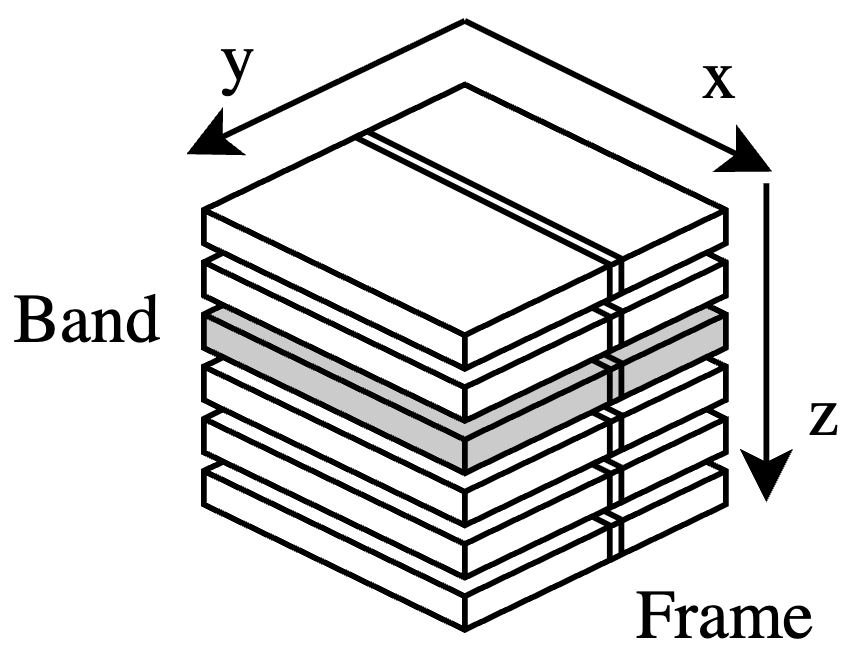
\includegraphics[width=0.3\textwidth]{figures/hsi.png}
	\end{center}
	\caption{}
	\label{fig:hsi}
\end{figure}

\newpage
of

\begin{figure}[ht]
	\begin{center}
		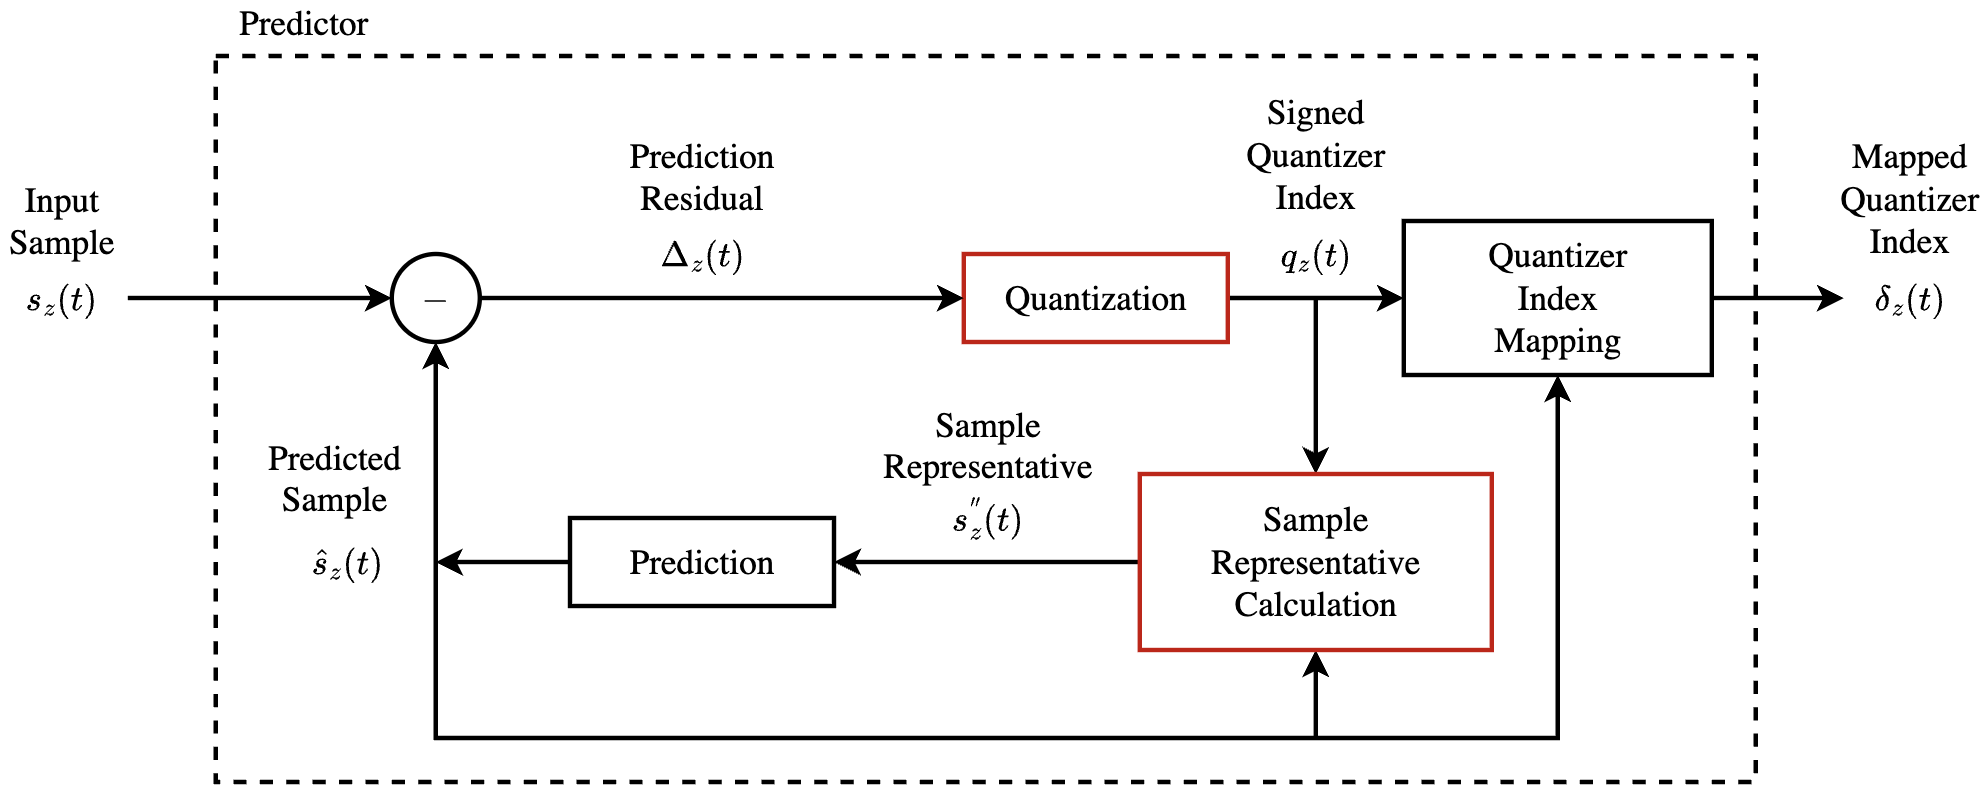
\includegraphics[width=0.9\textwidth]{figures/predictor-block.png}
	\end{center}
	\caption{}
	\label{fig:predictor-block}
\end{figure}

\newpage
multipage

\begin{figure}[ht]
	\begin{center}
		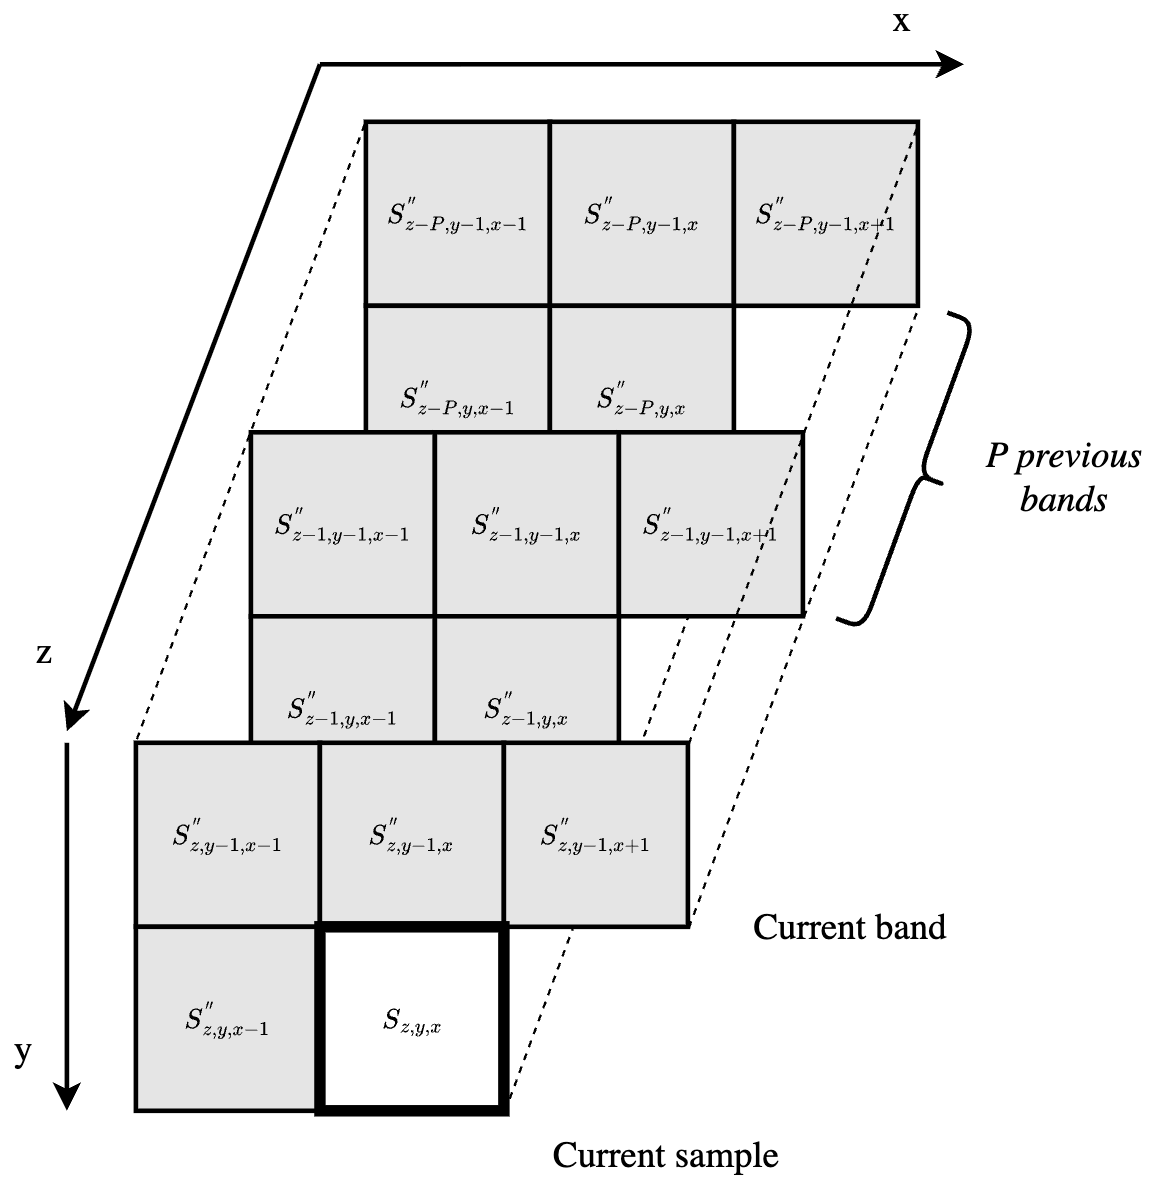
\includegraphics[width=0.7\textwidth]{figures/prediction-neighborhood.png}
	\end{center}
	\caption{}
	\label{fig:prediction-neighborhood}
\end{figure}

\begin{figure}[ht]
	\begin{center}
		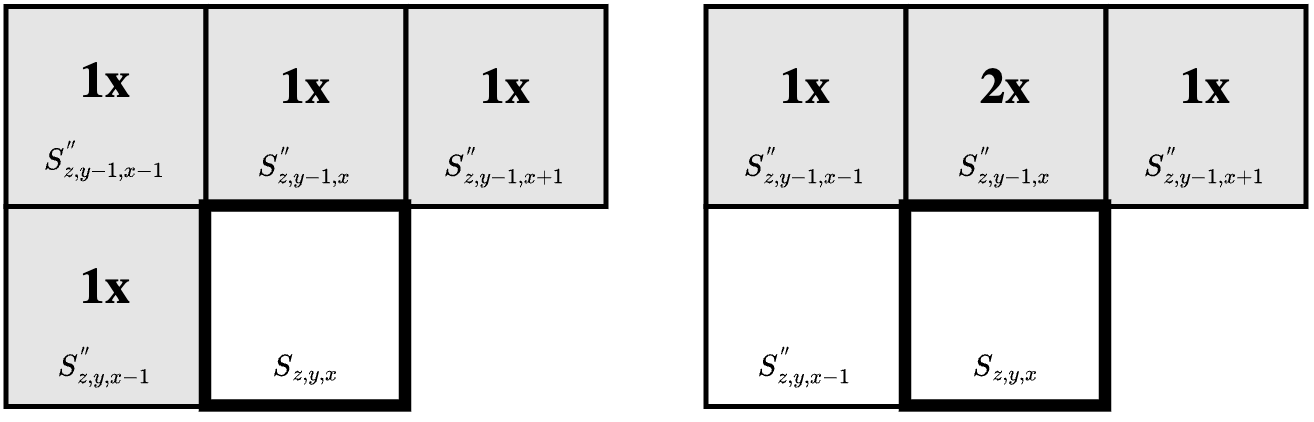
\includegraphics[width=0.7\textwidth]{figures/local-sums.png}
	\end{center}
	\caption{}
	\label{fig:local-sums}
\end{figure}

\begin{equation}
	\sigma_{z,y,x} =
	\begin{cases}
		s''_{z,\,y-1,\,x-1} + 2 s''_{z,\,y-1,\,x} + s''_{z,\,y-1,\,x+1},
		 & y > 0,\ 0 < x < N_X - 1,
		\\[6pt]
		4 s''_{z-1,\,y,\,x-1},
		 & y = 0,\ x > 0,\ z > 0,
		\\[6pt]
		2\!\left( s''_{z,\,y-1,\,x} + s''_{z,\,y-1,\,x+1} \right),
		 & y > 0,\ x = 0,
		\\[6pt]
		2\!\left( s''_{z,\,y-1,\,x-1} + s''_{z,\,y-1,\,x} \right),
		 & y > 0,\ x = N_X - 1,
		\\[6pt]
		4 s_{\text{mid}},
		 & y = 0,\ x = 0,\ z = 0.
	\end{cases}
	\label{eq:}
\end{equation}

\begin{equation}
	\mathbf{U}_z(t) =
	\begin{bmatrix}
		d_{z-1}(t)     \\
		d_{z-2}(t)     \\
		\vdots         \\
		d_{z-P^*_z}(t) \\
	\end{bmatrix},
	\label{eq:local-differences}
\end{equation}

\begin{equation}
	P^*_z = \min(z, P),
	\label{eq:prediction-bands}
\end{equation}

\begin{equation}
	\hat{d}_z(t) = \mathbf{W}_z(t) \cdot \mathbf{U}_z(t).
	\label{eq:predicted-central-local-difference}
\end{equation}

\begin{equation}
	\mathbf{W}_z(t)=
	\begin{bmatrix}
		\omega_z^{(1)}(t) \\
		\omega_z^{(2)}(t) \\
		\vdots            \\
		\omega_z^{(P^*_z)}(t)
	\end{bmatrix},
	\label{eq:weight-vector}
\end{equation}

\begin{equation}
	\omega_z^{(1)}(1) = \frac{7}{8} 2^{\Omega}, \qquad
	\omega_z^{(i)}(1) = \left\lfloor \frac{1}{8}\, \omega_z^{(i-1)}(1) \right\rfloor,
	\quad i = 2,3,\ldots,P_z^{*},
	\label{eq:weight-init}
\end{equation}

\begin{equation}
	\omega_{\mathrm{min}} = -2^{\Omega+2}, \: \omega_{\mathrm{max}} = -2^{\Omega+2} - 1.
	\label{eq:weight-min-max}
\end{equation}

\begin{equation}
	\omega^{(i)}_{z, \text{offset}}(t) = \left\lfloor \frac{1}{2} \left(2^{-\rho(t)} \cdot d_{z-i}(t) \cdot \text{sgn}^+[e_z(t)] + 1 \right) \right\rfloor,
	\label{eq:weight-offset}
\end{equation}

\begin{equation}
	e_z(t) = 2s'_z(t) - \tilde{s}_z(t).
	\label{eq:double-resolution-prediction-error}
\end{equation}

\begin{equation}
	\rho(t) = \operatorname{clip}\!\left(
	\nu_{\min} +
	\left\lfloor \frac{t - N_x}{t_{\mathrm{inc}}} \right\rfloor,
	\{ \nu_{\min}, \nu_{\max} \}
	\right)
	+ D - \Omega,
	\label{eq:weight-update-scaling-exponent}
\end{equation}

\begin{equation}
	\omega^{(i)}_z(t + 1) = \text{clip} \left( \omega^{(i)}_z(t) + \omega^{(i)}_{z, \text{offset}}(t), \{ \omega_{min}, \omega_{max} \} \right),
	\label{eq:weight-update}
\end{equation}


\begin{figure}[ht]
	\begin{center}
		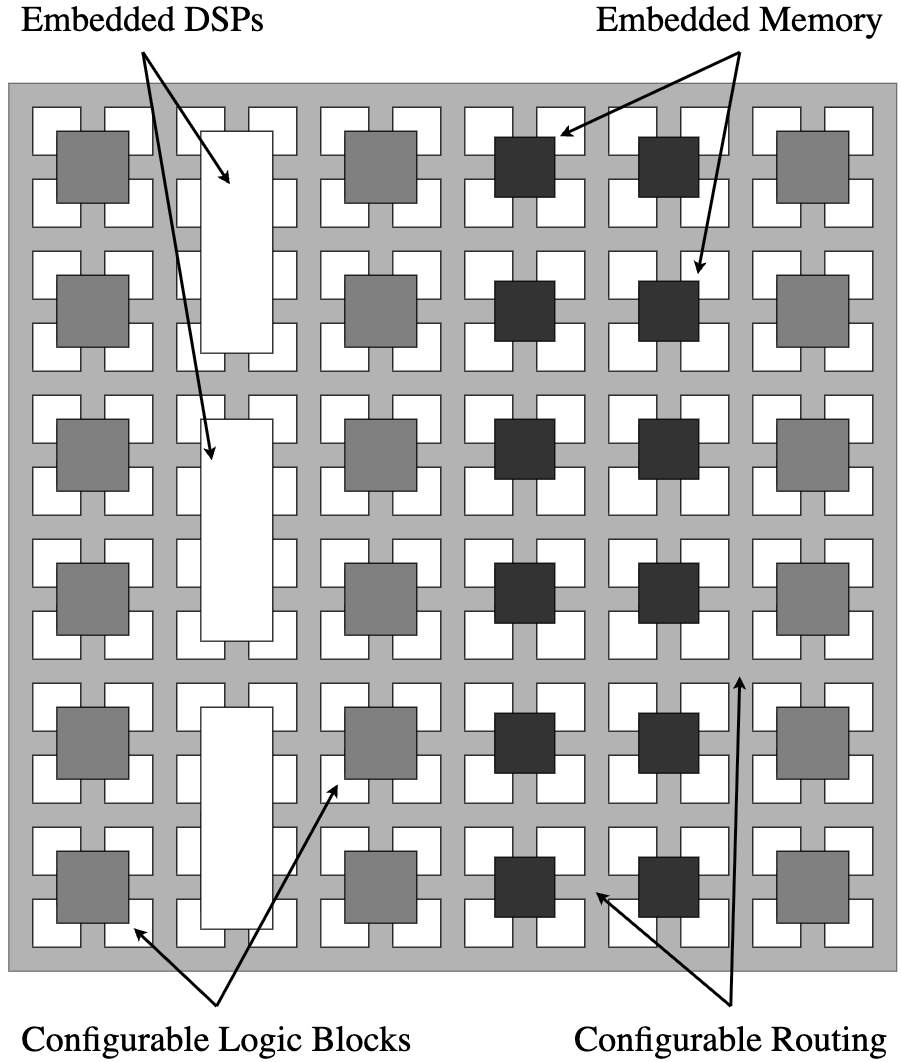
\includegraphics[width=0.55\textwidth]{figures/fpga.png}
	\end{center}
	\caption{}
	\label{fig:fpga}
\end{figure}

\chapter{State-of-the-Art}
\label{sec:state-of-the-art}

Since the release of the issue 1 standard, several implementations for hardware have been developed. Due to the lossless operation of the algorithm, image samples are used in place of the sample representatives of issue 2. This allows samples of different bands to be processed in parallel execution pipelines, an approach used by \citeauthor{orlandicParallelFPGAImplementation2019} to achieve a throughput of 750 MS/s \cite{orlandicParallelFPGAImplementation2019}. Samples are processed in the \acrshort{BIP} ordering, where image pixels are processed sequentially. Groups of $N_p$ samples are split according to their band and processed by $N_p$ pipelined cores. A different approach is used by \citeauthor{tsigkanosHighPerformanceCOTSFPGA2020}, in which images are split into segments that are compressed using separate, simpler cores. Using five parallel cores, a throughput of 1387 MS/s is reached.

Both of the mentioned issue 1 implementations support on-the-fly (real-time) processing, in which samples are processed immediately as they are made available from the image sensor. This is a desirable feature that reduces the need for temporary data storage. For the \acrshort{hypso}-1 image sensor, the real-time processing requirement is about 110.6 MS/s when operating at its maximum capacity of 47 frames per second with frames of size $1936x1216$ samples \cite{grotteOceanColorHyperspectral2022}. The real-time requirement differs between sensors, with the sensors of AVIRIS-NG and CHIME residing at 37.5 MS/s and 125 MS/s respectively \footnote{add cite to 18 and 21 from Bascones paper}[].

The quantization step, and subsequent sample representatives, of issue 2 introduce data dependencies in the predictor stage (\autoref{fig:dependencies}) that pose a challenge for pipelined hardware implementations. Parallel processing of samples using the method of \citeauthor{orlandicParallelFPGAImplementation2019} is no longer possible. \citeauthor{barriosHardwareImplementationCCSDS2021} present the first implementation of issue 2 in open literature, and is fully compliant with the standard \cite{barriosHardwareImplementationCCSDS2021}. Using the \acrshort{HLS} design methodology, they reach a low throughput of 18 MS/s. No special considerations as to the data dependencies are made, resulting in an almost fully serial implementation. This shows that a different approach is required to reach real-time operation. For the keen reader, a detailed of summary of key design specs of the following issue 2 implementations is presented in \autoref{tab:throughputs}. The table will also be discussed at the end of the chapter.

\begin{table}[ht]
	\caption{The number of processed samples interleaving $z-1$ and $t-1$ dependencies, including the novel FID ordering in addition to the standard orderings.}
	\label{tab:orderings-fid}
	\begin{center}
		\begin{tabular}{l l l l l l}
			\hline
			      & \textbf{BSQ}    & \textbf{BIP} & \textbf{BIL} & \textbf{FID} \\
			\hline
			$z-1$ & $N_x \cdot N_y$ & $1$          & $N_x$        & $N_z - 1$    \\
			$t-1$ & $1$             & $N_z$        & $1$          & $N_z$        \\
			\hline
		\end{tabular}
	\end{center}
\end{table}

As shown in \autoref{sec:compression}, data dependencies may be selectively bypassed by carefully selecting the sample processing order. This interleaves data dependant calculations by a number of other samples, allowing time for the dependency to resolve. The first viable real-time implementation of issue 2 is presented by \citeauthor{basconesFPGAAcceleratorRealTime2020}. By use of a novel sample processing order, dubbed \acrfull{FID}, they reach a throughput of 285 MS/s. \autoref{fig:fid} shows a visualization of the \acrshort{FID} processing order, with processed samples marked in white. Frames are concatenated along the $x$ dimension and processed diagonally, iterating on the $z$ and $x$ dimensions. The number of samples that interleave data dependencies can be obtained by counting along the diagonal, giving $N_z-1$ and $N_z$ samples for $z-1$ and $t-1$ dependencies respectively. This facilitates the deep pipeline of $57$ stages used by the implementation while allowing support for full and reduced prediction modes and all local sum types. Dependency interleaving of the different processing orders, including \acrshort{FID} is summarized in \autoref{tab:orderings-fid}.

The use of a new processing ordering requires reordering buffers that convert from the standard \acrshort{BIP} ordering. These are placed at each side of the predictor. The hybrid encoder module proceeds in \acrshort{BIP} ordering to result in a compressed bitstream compliant with the standard. Additionally, this allows integration into existing systems. The reordering buffers come at the cost of extra hardware resources, resulting in a somewhat larger footprint than that of \citeauthor{barriosHardwareImplementationCCSDS2021}. Especially in terms of \acrshort{BRAM}, which is increased from $85$ to $213$ due to storage required by the reordering buffers. Resource utilization is somewhat mitigated by use of portable \acrshort{RTL} written in VHDL, as opposed to the \acrshort{HLS} approach used by \citeauthor{barriosHardwareImplementationCCSDS2021}. Both implementations support runtime reconfiguration, adding additional hardware to provide flexibility.

\begin{figure}[ht]
	\begin{center}
		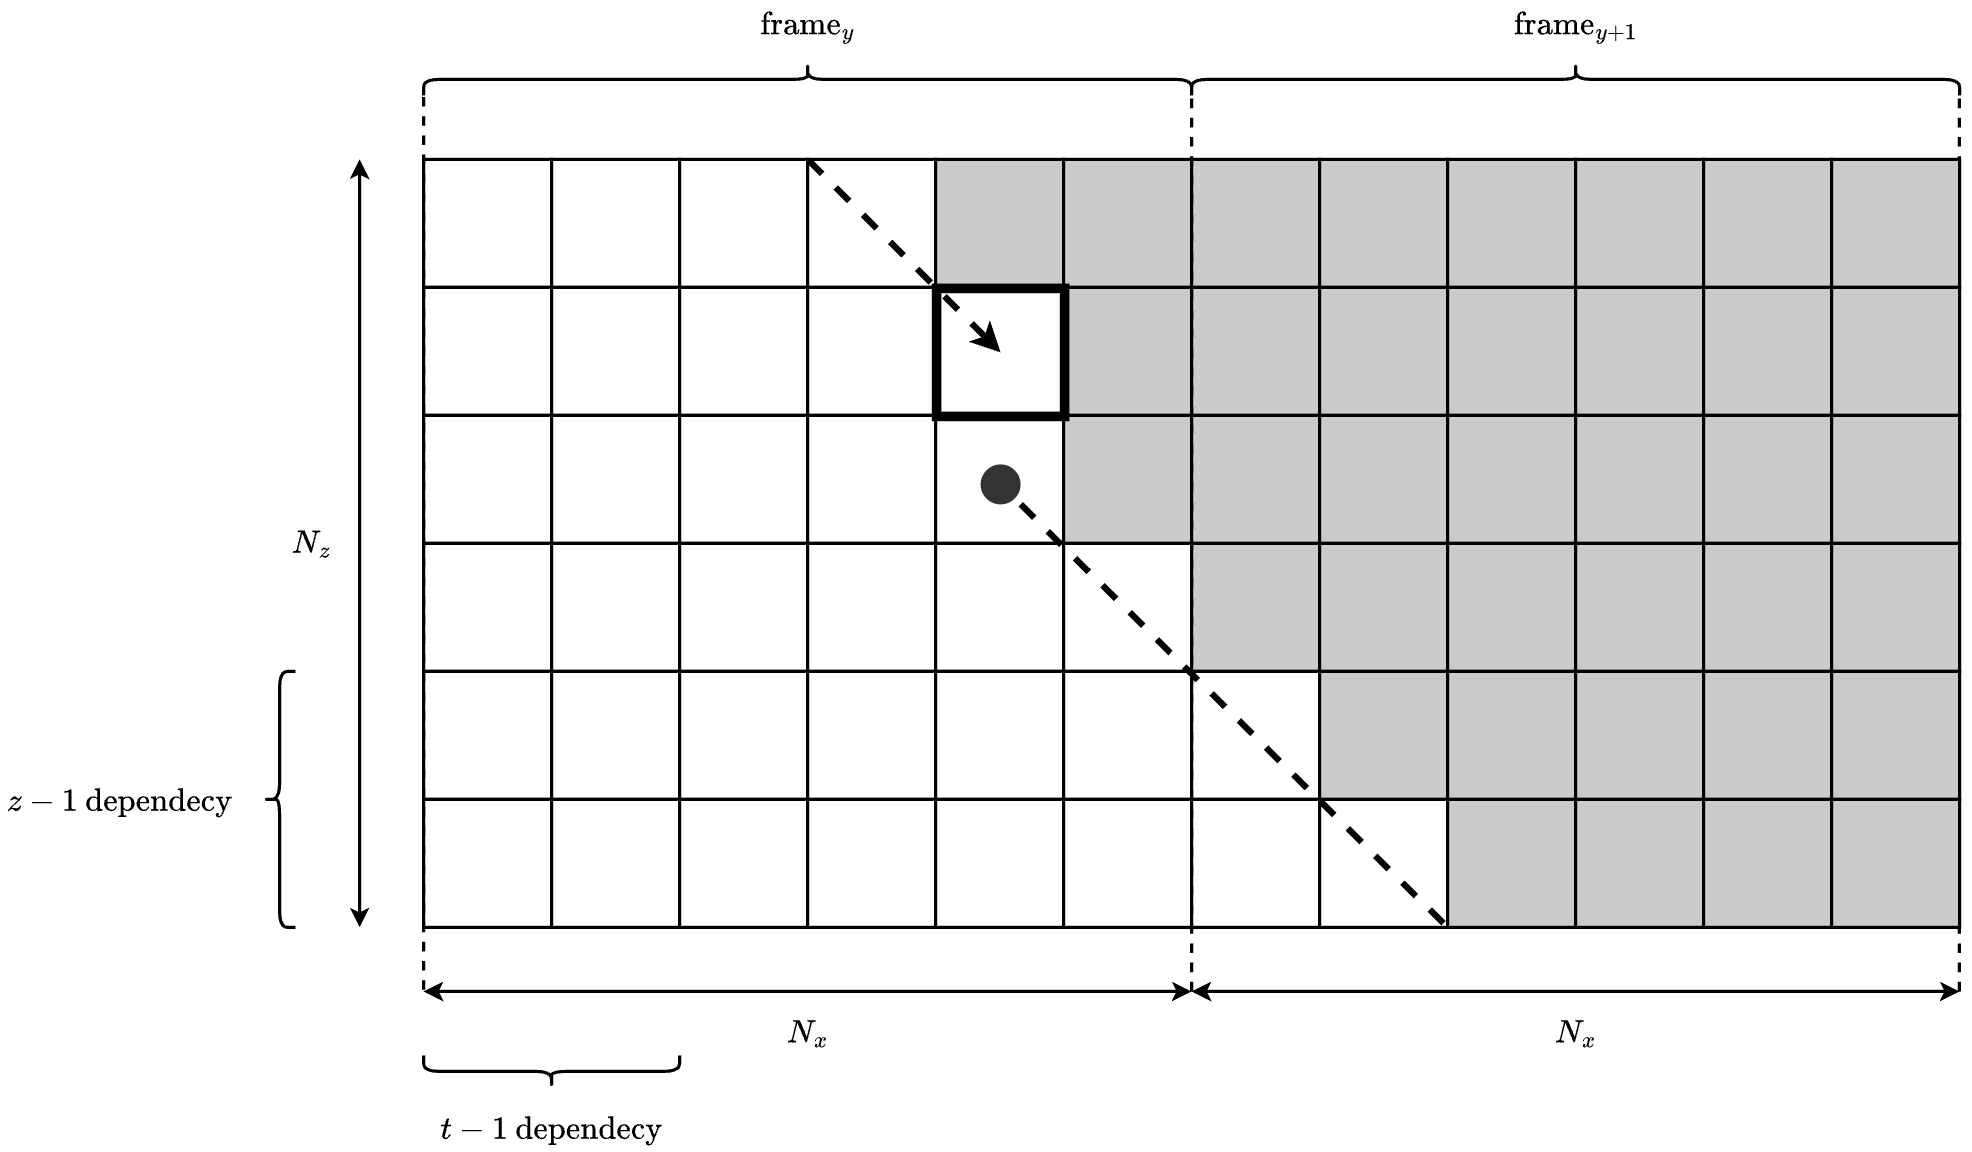
\includegraphics[width=1\textwidth]{figures/fid.png}
	\end{center}
	\caption{Novel \acrshort{FID} processing order presented by \citeauthor{basconesFPGAAcceleratorRealTime2020} interleaves all dependencies by a minimum of $N_z - 1$ samples, allowing deep pipelining.}
	\label{fig:fid}
\end{figure}

\begin{figure}[ht]
	\begin{center}
		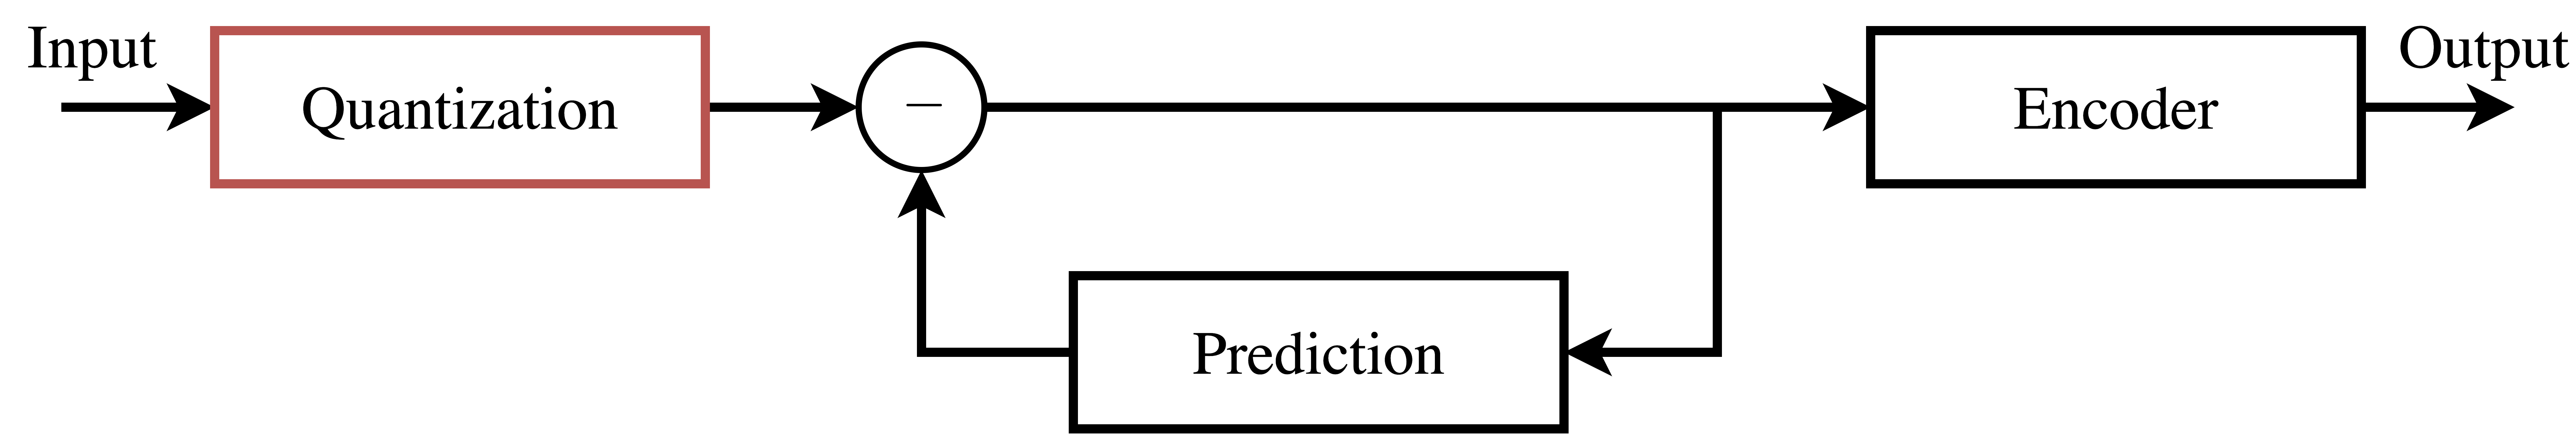
\includegraphics[width=0.9\textwidth]{figures/ccsds-prequantization.png}
	\end{center}
	\caption{Prequantization of image samples allows use of a lossless prediction loop, avoiding the challenging data dependencies.}
	\label{fig:prequantization}
\end{figure}

The works by \citeauthor{chatziantoniouScalableDataRateNearLossless2022a} and \citeauthor{valsesiaHighThroughputOnboardHyperspectral2019} suggest that the quantization step of the issue 2 predictor can be moved prior to the predictor as shown in \autoref{fig:prequantization} \cite{chatziantoniouScalableDataRateNearLossless2022a, valsesiaHighThroughputOnboardHyperspectral2019}. Image samples are quantized prior to prediction. This allows use of a lossless prediction loop, avoiding the need for sample representatives and the challenging data dependencies. The predictor can now be implemented using similar techniques as used by implementations of issue 1.

In addition to prequantization, \citeauthor{chatziantoniouScalableDataRateNearLossless2022a} employ image segmentation, a technique that may also be used by issue 2 compliant compressors as described in issue 2 green book \cite{LosslessMultispectralHyperspectral2022}. Reduction in compression performance is minimal for the segmented image, given that the segment sizes are large. Using VHDL \acrshort{RTL} and five cores, \citeauthor{chatziantoniouScalableDataRateNearLossless2022a} reach a throughput of 1375 MS/s, with a single core performance of 285 MS/s. This matches the results of \citeauthor{basconesRealTimeFPGAImplementation2022}, but at a larger area footprint.

Prequantization comes at a degradation in compression performance, both in terms of bitrate and image distortion, as opposed to the in-loop quantizer of issue 2. The works by \citeauthor{chatziantoniouScalableDataRateNearLossless2022a} and \citeauthor{valsesiaHighThroughputOnboardHyperspectral2019} show that the increase in bitrate and decreased image SNR are greatest for low bitrates. To combat this, \citeauthor{valsesiaHighThroughputOnboardHyperspectral2019} suggest using an on-ground computational neural network (CNN) to reconstruct lost data. During simulation, the method is able to mitigate data loss, and may be used for in-loop quantization as well as prequantization. However, the approach adds significant complexity to the reconstruction of images.

\begin{figure}[ht]
	\begin{center}
		
\includegraphics[width=1\textwidth]{figures/ccsds-pipeline-naive.png}
	\end{center}
	\caption{Suggested pipeline using reduced prediction mode, narrow local sums and \acrshort{BIL} processing order. Weight updates depend on results from the sample representative calculation, constraining the throughput.}
	\label{fig:ccsds-pipeline-naive}
\end{figure}

\citeauthor{sanchezReducingDataDependencies2022} identify that by using narrow local sums and reduced prediction mode, $t-1$ dependencies related to local sums and differences can be avoided (\autoref{fig:local-sums}) \cite{sanchezReducingDataDependencies2022}. Additionally, by using \acrshort{BIL} processing order, $z-1$ dependencies can be avoided (\autoref{tab:orderings-fid}). \autoref{fig:ccsds-pipeline-naive} shows a pipeline using these configuration. The weight update calculation, required by predicted central local differences, still has an unavoidable $t-1$ dependency, placing a significant restriction on the achievable throughput.

\citeauthor{barriosRemovingDataDependencies2024} present a solution in which the remaining data dependence of the weight updates is avoided by skipping weight updates entirely. This allows deep pipelining, but comes at the cost of reduced compression performance as the prediction loop can no longer dynamically adapt to image characteristics. To mitigate this, the authors use previous data sets to carefully select the initial weight values for specific image sensors. The analysis is based on compression for a set of absolute error limits, $\{0,1,3,7,15,31\}$, with performance penalties depending heavily on the image set. For some configurations the compress performance is even improved with up to $10\%$, but for most a worsening in the range $2-10\%$.

\citeauthor{sanchezReducingDataDependencies2022} also present a mathematically equivalent way of calculating the sign of the double-resolution prediction error $e_z(t)$, given by

\begin{equation}
	\text{sgn}^+\bigl[e_z(t)\bigr] =
	\begin{cases}
		-1,                                            & \text{if }\lvert s_z(t) - \hat{s}_z(t) \rvert \le m_z(t)\ \text{and }\tilde{s}_z(t)\text{ is odd},  \\[6pt]
		1,                                             & \text{if }\lvert s_z(t) - \hat{s}_z(t) \rvert \le m_z(t)\ \text{and }\tilde{s}_z(t)\text{ is even}, \\[6pt]
		\text{sgn}^+\bigl[s_z(t) - \hat{s}_z(t)\bigr], & \text{otherwise}.
	\end{cases}
	\label{eq:math-opt}
\end{equation}

This removes the dependence of the clipped quantizer bin center (\autoref{eq:double-resolution-prediction-error}), calculated in the samples representative stage, allowing calculation to start earlier (\autoref{fig:ccsds-pipeline-math-opt}). By speculatively calculating the weight updates for the two possible outcomes of the sign, weight updates may be calculated in parallel with the sign during the prediction stage. Once the sign calculation resolves, the correct outcome of the weight update is selected and passed to the predicted central local difference stage. This approach, dubbed the mathematical optimization approach, is evaluated by \citeauthor{barriosRemovingDataDependencies2024} using the \acrshort{HLS} methodology. Only the predictor module is evaluated, reaching a throughput of 231 MS/s. This is used as comparison for their approach of skipping weight updates, which reaches 236 MS/s. For both methods, only the predictor is implemented.

\begin{figure}[ht]
	\begin{center}
		\includegraphics[width=1\textwidth]{figures/ccsds-pipeline-math-opt.png}
	\end{center}
	\caption{Weight update dependence on sample representatives is alleviated using the mathematical optimization approach suggested by \citeauthor{sanchezReducingDataDependencies2022}. Speculative calculation of weight updates further increases throughput.}
	\label{fig:ccsds-pipeline-math-opt}
\end{figure}

The mathematical optimization approach is used by \citeauthor{vorhaugHyperspectralImageCompression2024} to develop a full issue 2 accelerator for use on-board the \acrshort{hypso} missions \cite{vorhaugHyperspectralImageCompression2024}. By use of VHDL \acrshort{RTL}, the design reaches a throughput of 110 MS/s on the Kintex XCKU040 \acrshort{FPGA}, the same \acrshort{FPGA} used in the evaluations of the previously mentioned issue 2 implementations. However, for the Zynq-7030, used on-board \acrshort{hypso}-1 and 2, a modest throughput of 67 MS/s is reached. This does not fulfill the real-time requirement of the \acrshort{hypso}-1 image sensor of 110.6 MS/s. The design is implemented without support for runtime configuration, resulting in the smallest compressor in open literature in terms of resource utilization.

\begin{figure}[ht]
	\begin{center}
		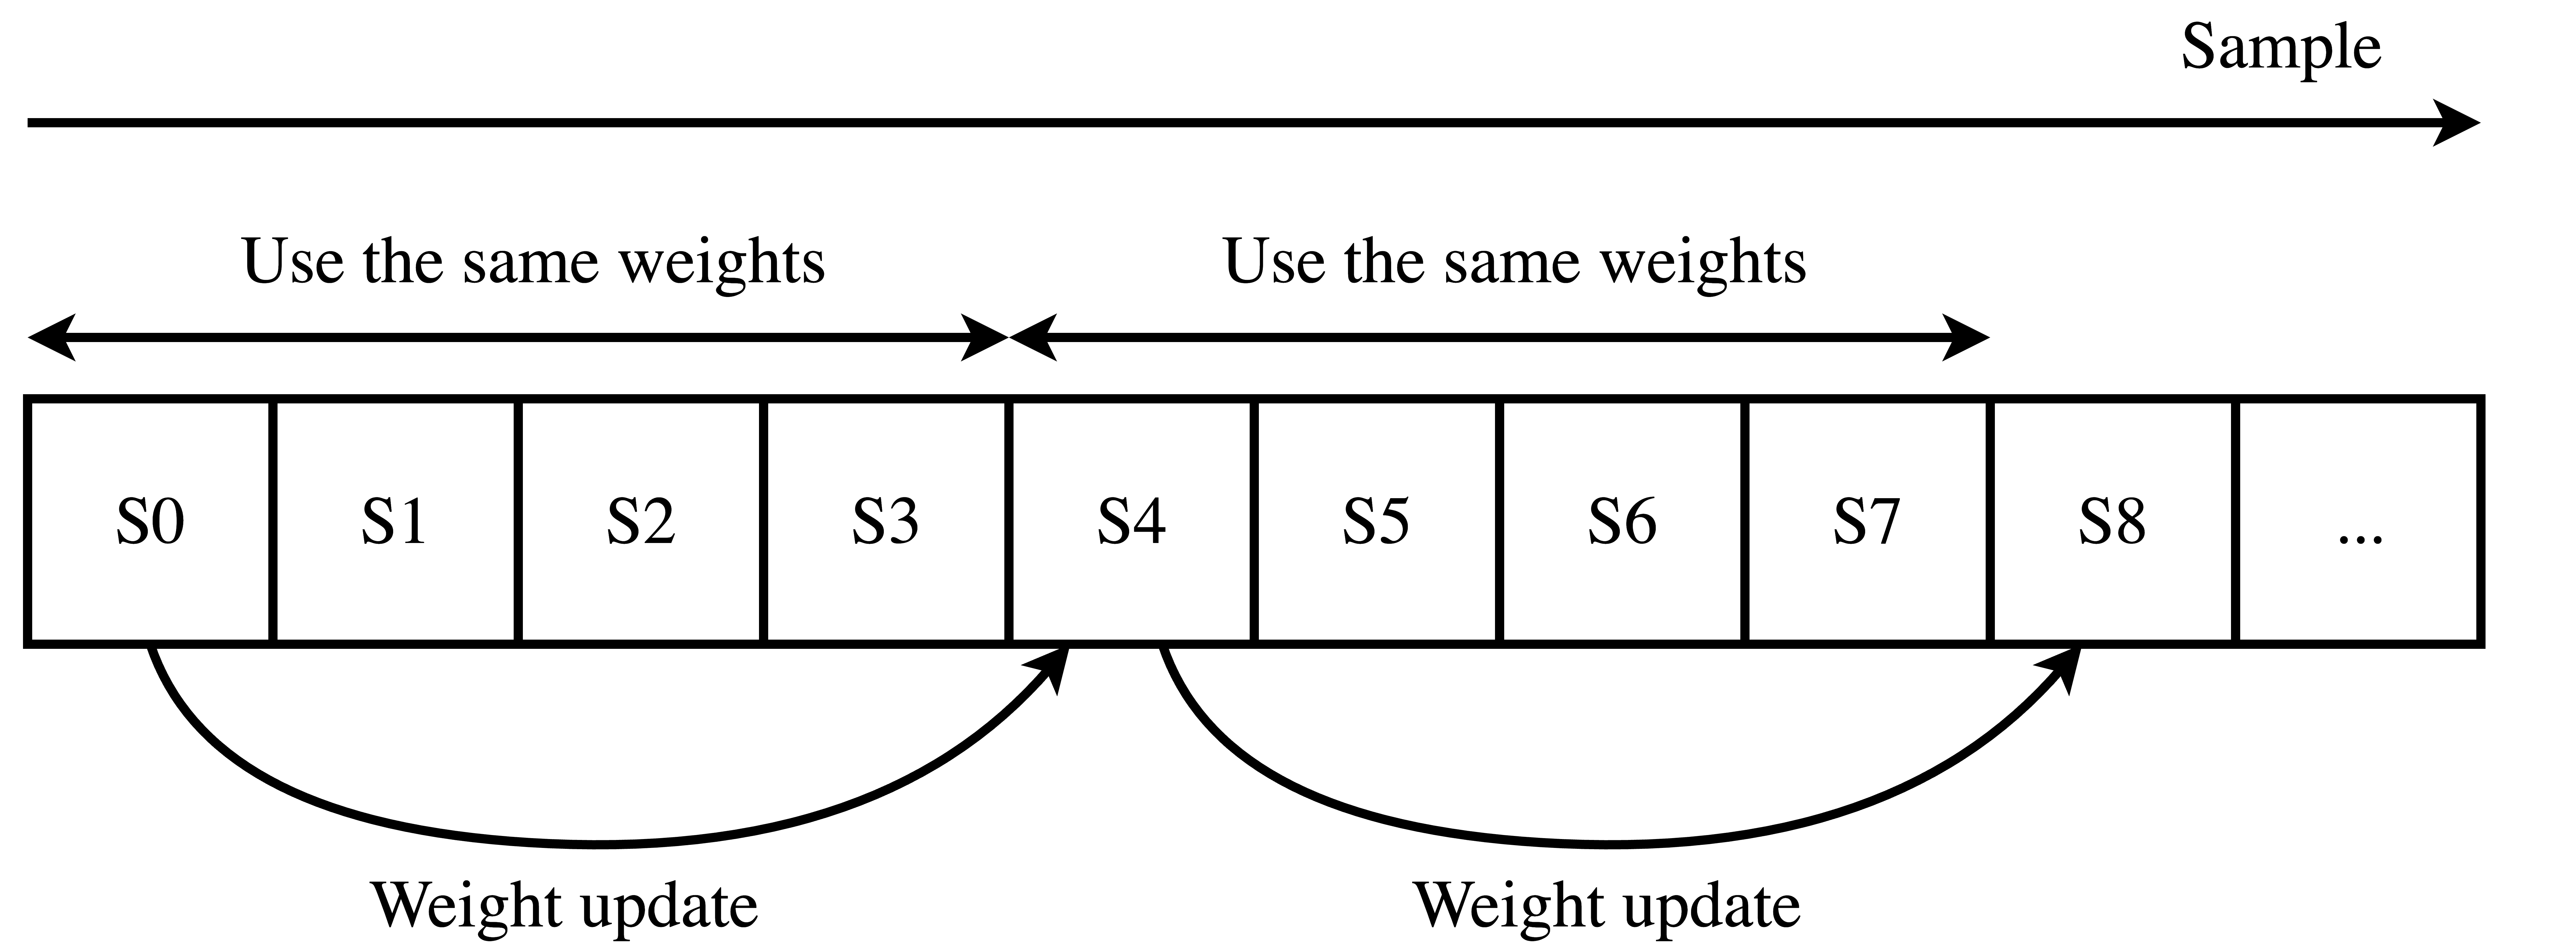
\includegraphics[width=0.8\textwidth]{figures/ccsds-weight-updates.png}
	\end{center}
	\caption{The proposed weight update scheme by \citeauthor{jiaRemovalFeedbackLoop2025}. Weights are kept unchanged for the first samples of every line, after which the sample from four samples earlier is used in the weight update calculation.}
	\label{fig:delayed-weight-updates}
\end{figure}

The achievable throughput of the mathematical optimization approach is constrained by the indivisible weight update calculation. To alleviate the problem, \citeauthor{jiaRemovalFeedbackLoop2025} suggest a modified weight update scheme, dubbed delayed weight updates \cite{jiaRemovalFeedbackLoop2025}. Their predictor is implemented using VHDL \acrshort{RTL}, reaching a throughput of 348 MS/s, while maintaining a small area footprint. Note that this result is achieved using a different \acrshort{FPGA}, Zynq XCZU5EV, than the previous works. Delayed weight updates come at slight degradation in compression performance. The analysis made by \citeauthor{jiaRemovalFeedbackLoop2025} is made using data sets from known missions, such as AVIRIS, over a set of absolute error limits, $\{0,1,3,7,15\}$. Results show a reduction in compression ratio in the range $1-5\%$, outperforming the approach of skipping weight updates as suggested by \citeauthor{barriosRemovingDataDependencies2024}.

\begin{equation}
	\omega^{(i)}_{z, \text{unclipped}}(t+1)=
	\begin{cases}
		\omega^{(i)}_z(t),                                                                                                                   & t \le 2,          \\[6pt]
		\omega^{(i)}_z(t-3) + \omega^{(i)}_{z, \text{offset}}(t-3),                                                                          & t = 3,            \\[6pt]
		\left\lfloor \dfrac{1}{2}\left(\omega^{(i)}_z(t-3) + \omega^{(i)}_{z, \text{offset}}(t-3) + \omega^{(i)}_z(t) \right) \right\rfloor, & \text{otherwise}.
	\end{cases}
	\label{eq:delayed-weight-updates}
\end{equation}

\begin{table}[ht]
	\caption{Hardware utilization and throughput of hardware accelerators of the issue 2 standard. The predictor module is the smallest and fastest in open litterature.}
	\label{tab:throughputs}
	\centering
	\begin{tabular}{l r r r r r r}
		\hline
		\textbf{Implementation}                                                                                      & \textbf{FPGA} & \textbf{LUT} & \textbf{FF} & \textbf{DSP} & \textbf{BRAM} & \textbf{Throughput} \\
		\hline
		Barrios et al.\ \cite{barriosHardwareImplementationCCSDS2021}                                                & XCKU040       & 17185        & 11915       & 63           & 85            & 18~MS/s             \\
		B\'ascones et al.\ \cite{basconesRealTimeFPGAImplementation2022}                                             & XQRKU060      & 16458        & 15707       & 30           & 187.5         & 285~MS/s            \\
		Chatziantoniou et al.\ \cite{chatziantoniouScalableDataRateNearLossless2022a} 1 core                         & XCKU040       & 18861        & 21395       & -            & 104           & 285~MS/s            \\
		Chatziantoniou et al.\ \cite{chatziantoniouScalableDataRateNearLossless2022a} 5 core                         & XCKU040       & 67362        & 68987       & -            & 306           & 1375~MS/s           \\
		S\'anchez et al.\ \cite{sanchezReducingDataDependencies2022, barriosRemovingDataDependencies2024}, predictor & XCKU040       & 19840        & 12970       & 33           & 213           & 231~MS/s            \\
		Barrios et al.\ \cite{barriosRemovingDataDependencies2024}, predictor                                        & XCKU040       & 11095        & 11729       & 20           & 186.5         & 236~MS/s            \\
		Vorhaug et al.\ \cite{vorhaugHyperspectralImageCompression2024}                                              & XCKU040       & 5577         & 2635        & 4            & 57.5          & 110~MS/s            \\
		Vorhaug et al.\ \cite{vorhaugHyperspectralImageCompression2024}                                              & XCZU7EV       & 5475         & 2635        & 4            & 57.5          & 141~MS/s            \\
		Jia et al.\ \cite{jiaRemovalFeedbackLoop2025}, predictor                                                     & XCZU5EV       & 3995         & 5050        & 7            & 94            & 348~MS/s            \\
		\hline
	\end{tabular}
\end{table}


\chapter{Previous Work}
\label{sec:previous-work}

This work builds upon, and aims to improve, the work of \citeauthor{vorhaugHyperspectralImageCompression2024} in \cite{vorhaugHyperspectralImageCompression2024}. \citeauthor{vorhaugHyperspectralImageCompression2024} implemented an issue 2 compliant hardware accelerator for use on-board the \acrshort{hypso} missions. The hardware accelerator was successfully integrated and tested on-board the \acrshort{hypso}-1 satellite, showing its viability for use. Before testing, the hardware was verified using a verification model, also written by \citeauthor{vorhaugHyperspectralImageCompression2024}. The following sections outlines the verification model and design of the hardware accelerator.

\subsection{Verification Model}

The verification model is implemented in the Python programming language and is fully compliant with the issue 2 standard. This includes support for all three entropy coders, full and reduced prediction mode, and all available local sum types. Since the purpose of the model is hardware verification, it saves intermediate values of the calculations and stores them in files. This results in large amounts of data to be stored in memory during execution, as well as written to the disk after completion. For this reason, the model is not suited for compression of full scale satellite images. Note that the verification model only implements compression, not decompression.

The model uses an object oriented programming style and consists of, in addition to a command line interface, three main modules: the header reader, predictor, and encoder. The header class stores the configuration used by the algorithm. Additionally it supports reading the configuration from files containing a header binary, optional tables and error limits. The raw image input of the compressor is passed to the predictor class which produces the mapped quantizer indices. These are passed to one of three encoder classes, depending on the selected entropy encoder. The header binary, produced by the header class, is prepended to the compressed image body before the result is stored to a file.

As the model is only intended for small test images, the calculations are implemented in a fully serial manner. All intermediary results are stored in global arrays that are modified in place. This removes the need for careful buffering of data that is needed by later calculations at the cost of massive penalties in memory usage. The use of large, global arrays also impacts execution time due to the constantly moving large chunks of data in and out the the memory caches. A final caveat is that modifying and accessing data in place makes the flow of the program harder to read, as function calls do not have clearly defined inputs and outputs at the call site.

\subsection{Hardware Accelerator}

The hardware accelerator uses the mathematical optimization approach suggested by \citeauthor{sanchezReducingDataDependencies2022}. \autoref{fig:vorhaug-block} shows a block diagram of the implementation. The implementation is only configurable using parameters in the \acrshort{RTL} code, and not at runtime. This allows high optimization by the synthesizer and \acrshort{PnR} tool, resulting in a small hardware area. Data is moved in and out of the module using the \acrshort{AXI} bus interface, which allows easy integration into the \acrshort{MPSoC} on-board \acrshort{hypso}. Because the implementation uses the \acrshort{BIL} processing order, as required by the mathematical optimization approach, the design features an optional reordering buffer. This module reorders from the \acrshort{BIP} used by the systems on \acrshort{hypso} to \acrshort{BIL} ordering.

\begin{figure}[ht]
	\begin{center}
		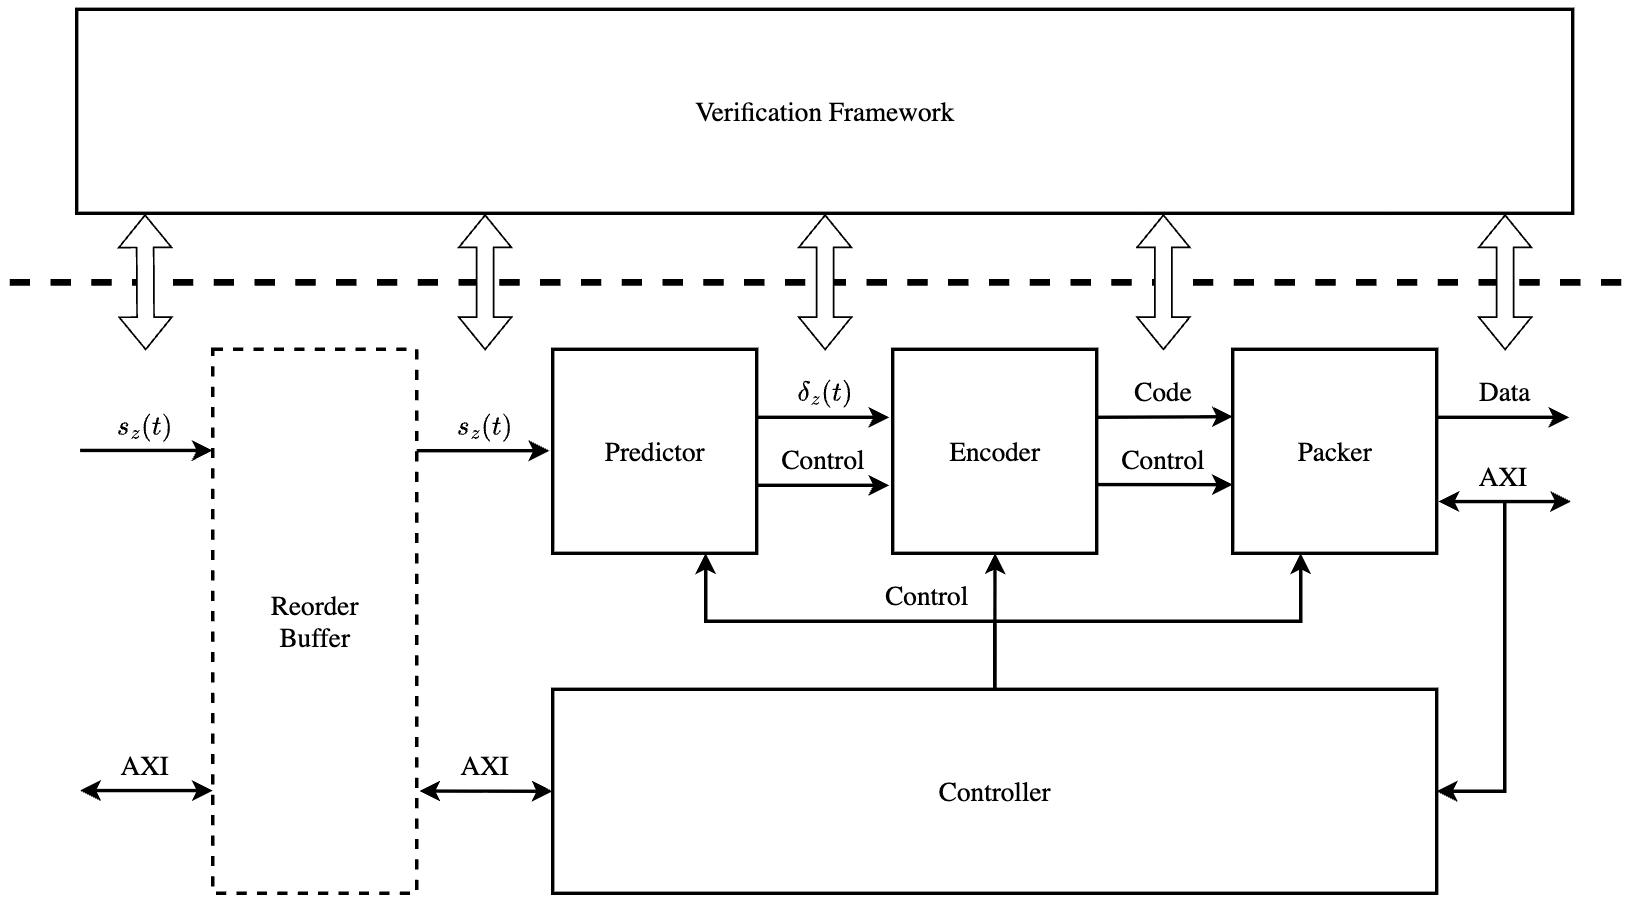
\includegraphics[width=1\textwidth]{figures/vorhaug-block.png}
	\end{center}
	\caption{Block diagram of \citeauthor{vorhaugHyperspectralImageCompression2024}. For easy integration into HYPSO, a reorder buffer reorders samples from \acrshort{BIP} to \acrshort{BIL}.}
	\label{fig:vorhaug-block}
\end{figure}

\begin{figure}[ht]
	\begin{center}
		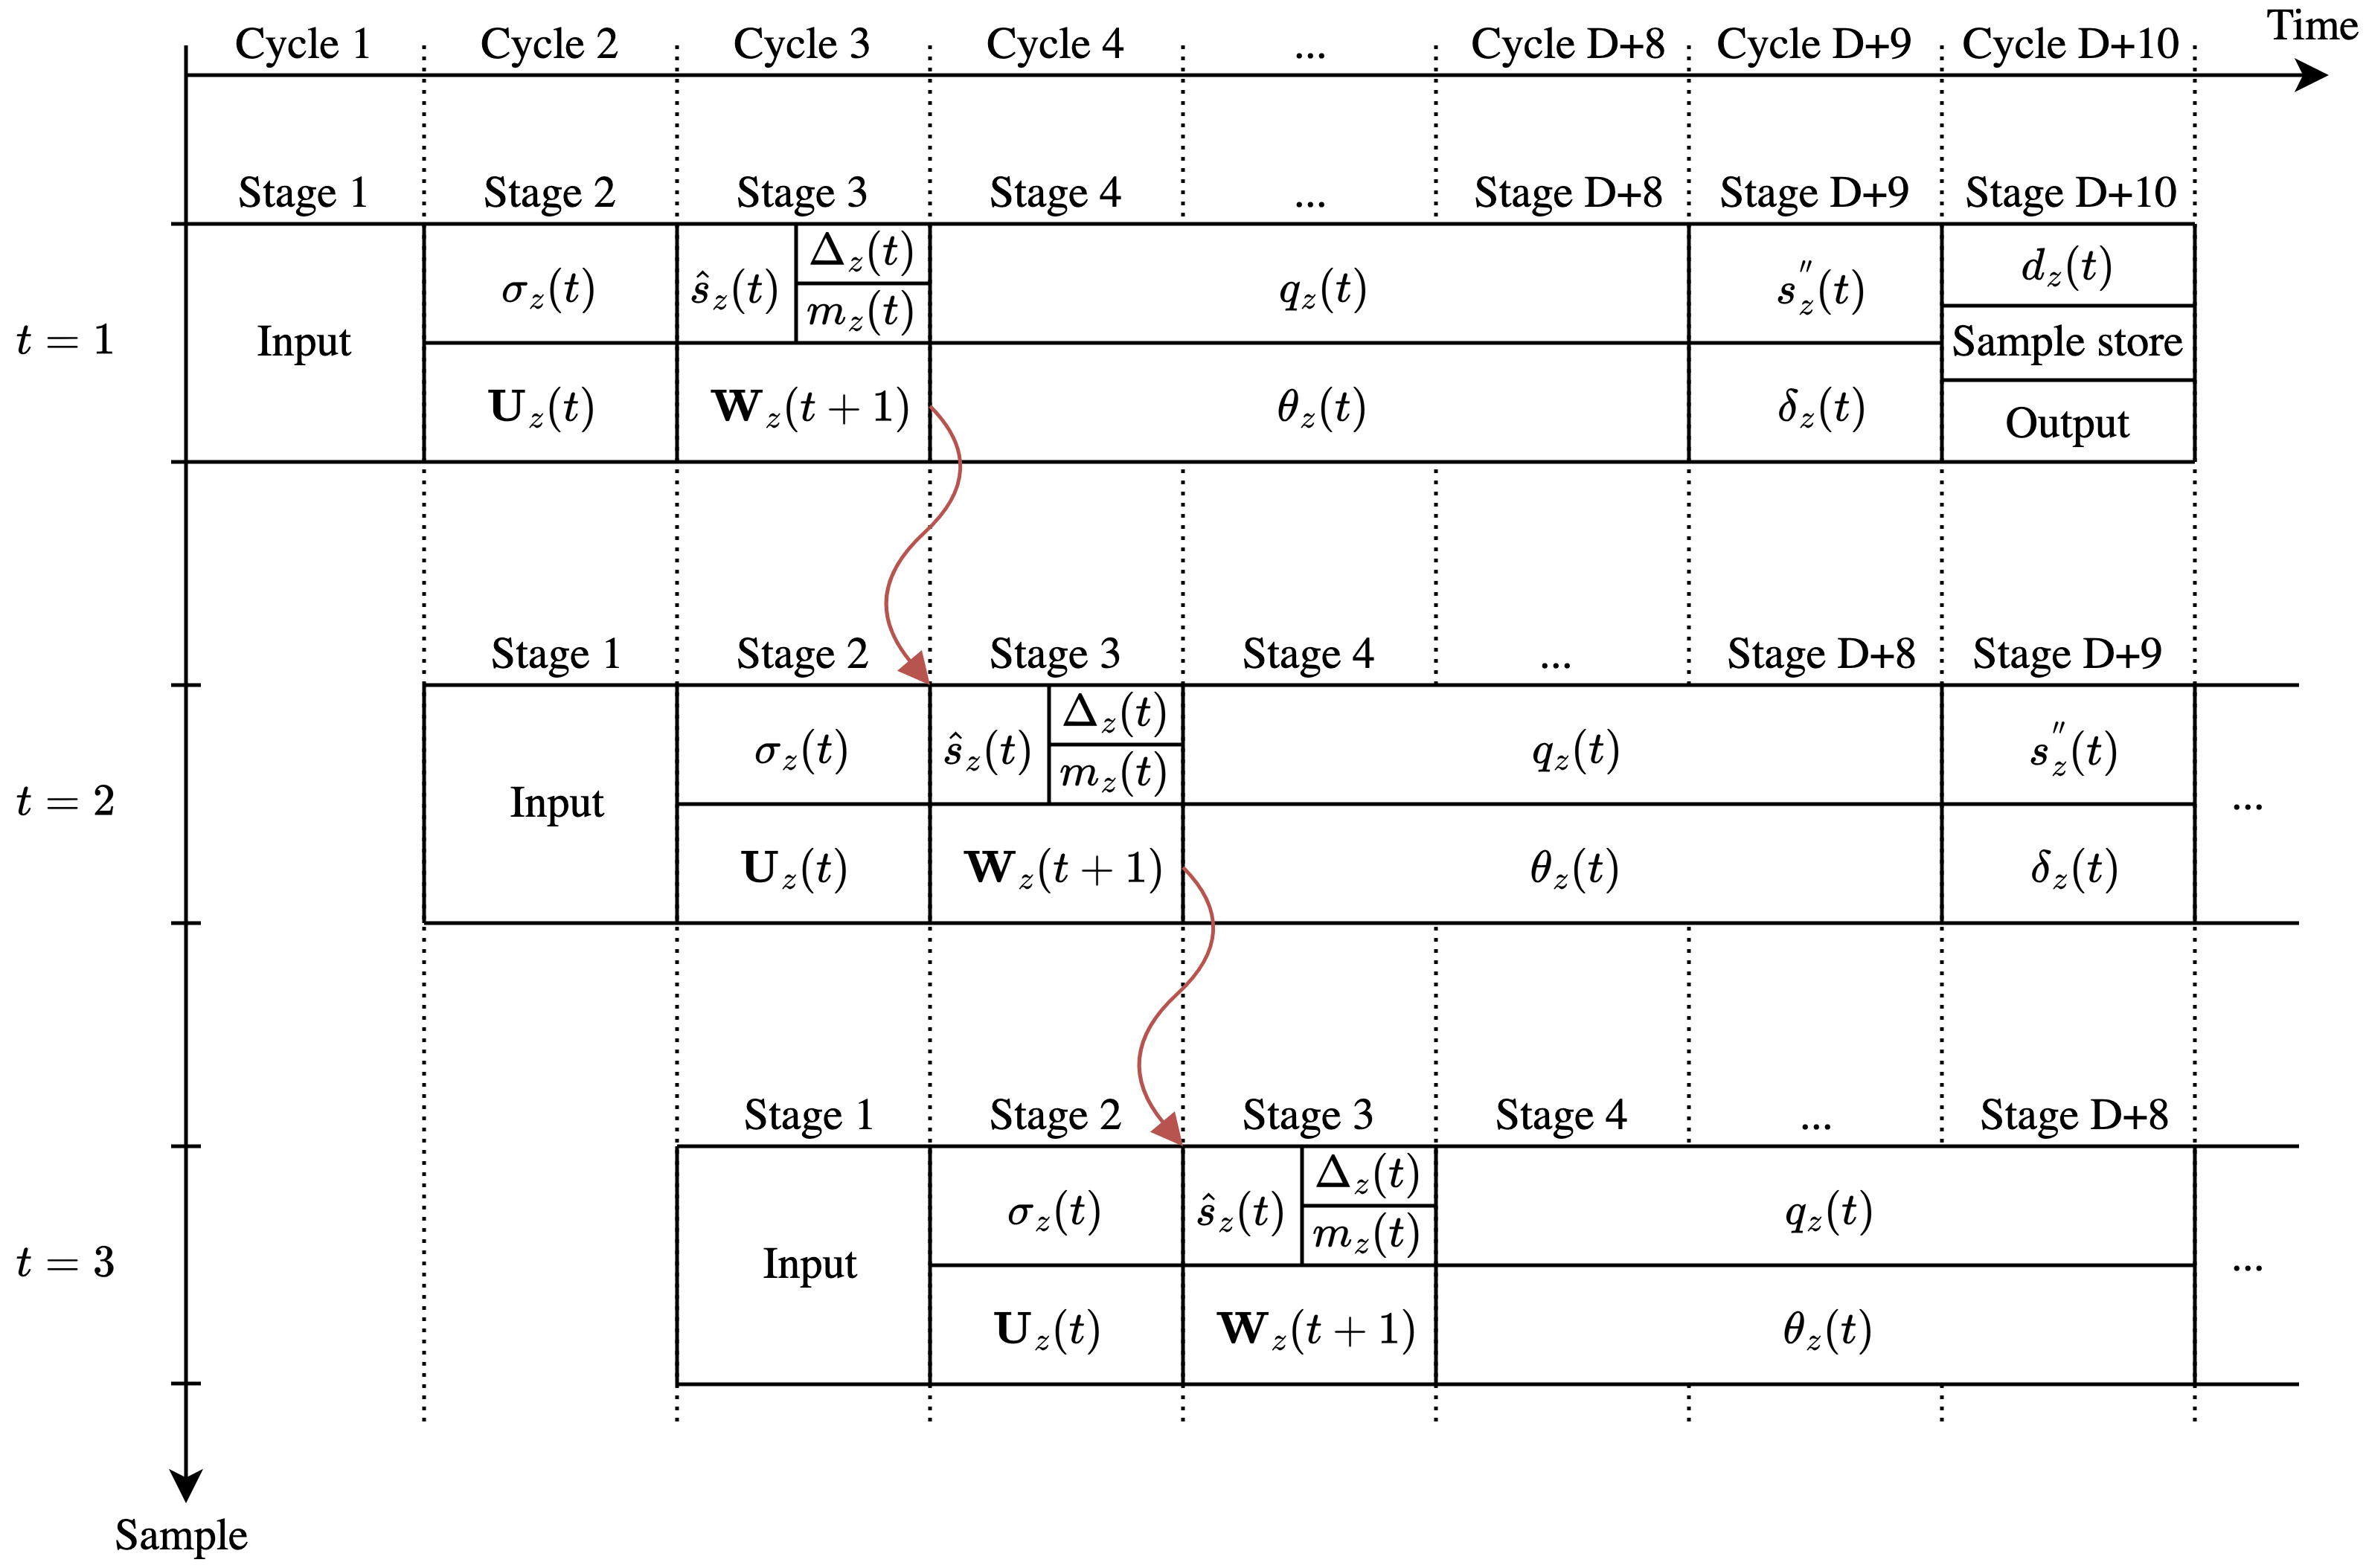
\includegraphics[width=1\textwidth]{figures/vorhaug-pipeline.png}
	\end{center}
	\caption{Full pipeline of \citeauthor{vorhaugHyperspectralImageCompression2024}. The indivisible weight update calculation in stage 3 restricts the throughput.}
	\label{fig:vorhaug-pipeline}
\end{figure}

\begin{figure}[ht]
	\begin{center}
		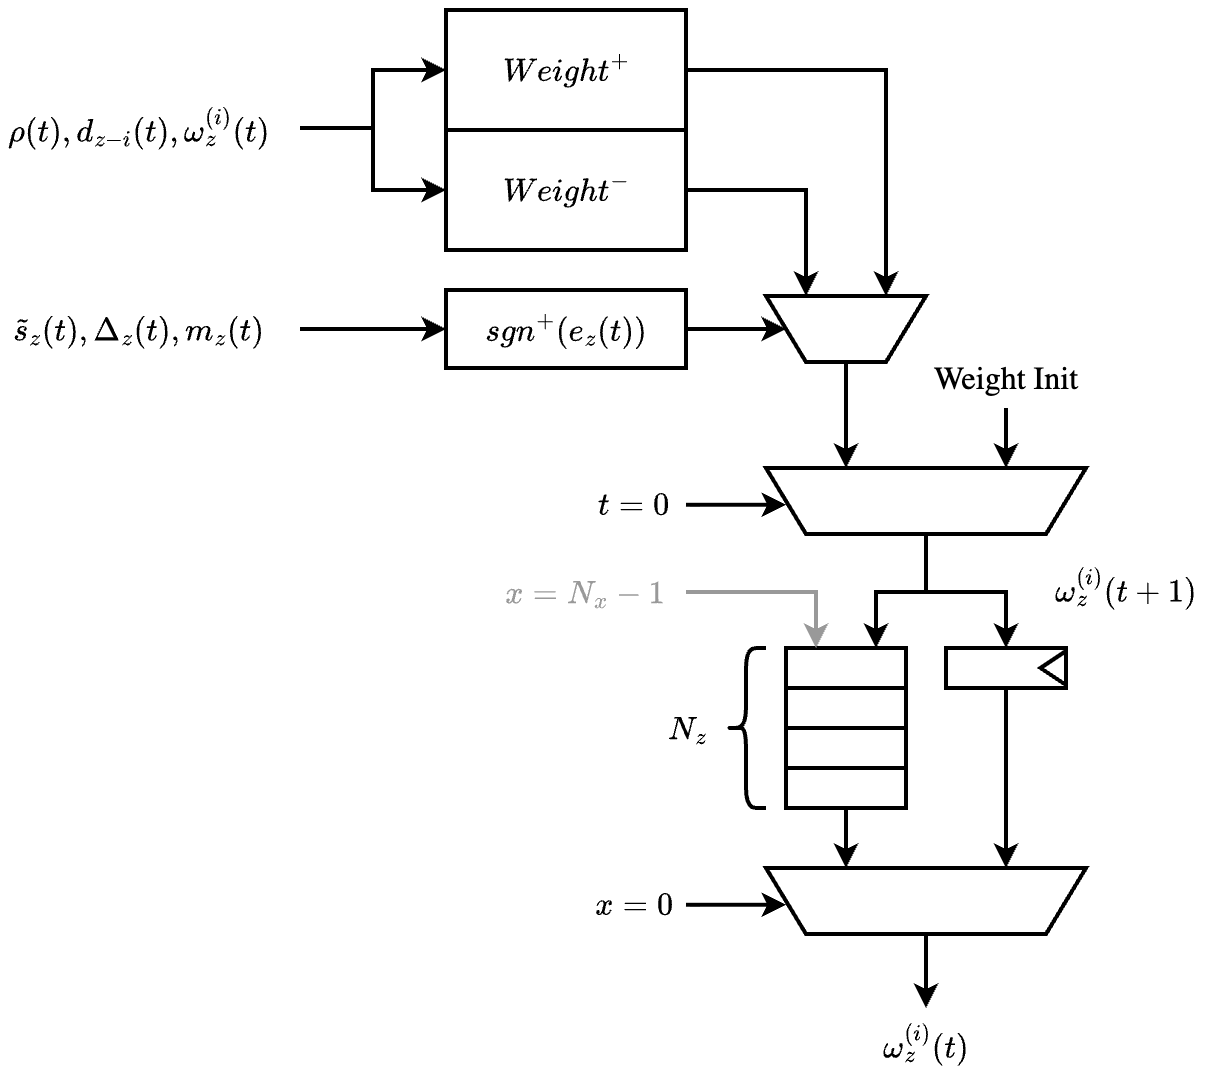
\includegraphics[width=0.8\textwidth]{figures/vorhaug-weights-hw.png}
	\end{center}
	\caption{Weight update stage of \citeauthor{vorhaugHyperspectralImageCompression2024} following the mathematical optimization approach proposed by \citeauthor{sanchezReducingDataDependencies2022}. Weight updates are calculated speculatively while the sign of the prediction error resolves.}
	\label{fig:vorhaug-weights-hw}
\end{figure}

\begin{figure}[ht]
	\begin{center}
		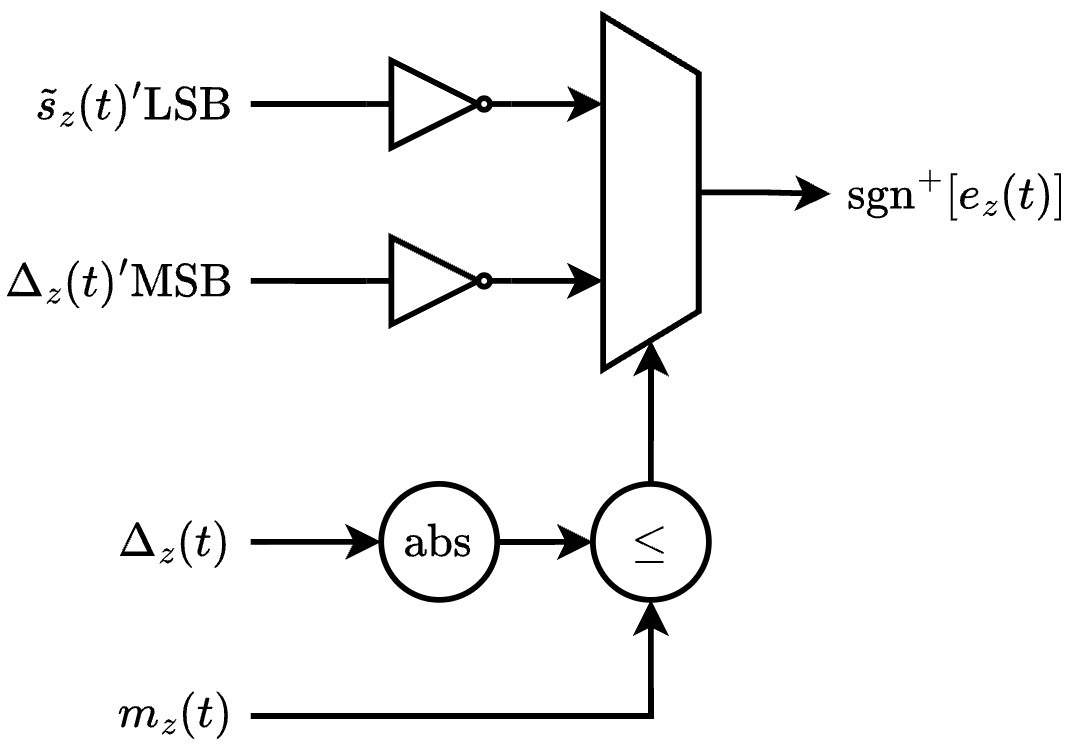
\includegraphics[width=0.5\textwidth]{figures/sign-block-diagram.png}
	\end{center}
	\caption{}
	\label{fig:sign-block-diagram}
\end{figure}

\begin{equation}
	\begin{cases}
		!\bigl(\tilde{s}_z(t)'{\mathrm{LSB}}\bigr), & \lvert \Delta_z(t) \rvert \le m_z(t), \\[6pt]
		!\bigl(\Delta_z(t)'{\mathrm{MSB}}\bigr),    & \text{otherwise}.
	\end{cases}
	\label{eq:sign-hw}
\end{equation}

\chapter{Implementation and Verification}
\label{sec:implementation}

This section outlines the integration of the new weight update scheme proposed by \citeauthor{jiaRemovalFeedbackLoop2025} into the hardware accelerator implemented by \citeauthor{vorhaugHyperspectralImageCompression2024}. The use of this new weight update scheme results in a compressor that is no longer compliant with the issue 2 standard. Because of this, the CNES decompressor can no longer be used to decompress, and thus verify, the results. No open-source issue 2 compliant decompressors are available, prompting the need for the development of such a tool. Before the changes to the hardware accelerator are presented, the outline for developing an open-source issue 2 decompressor is covered.

\section{Open-source Decompressor}

As shown in section \autoref{sec:compression}, the issue 2 compressor and decompressor have many similarities. This is especially true for the predictor stage, but also applies to the processing of header configuration. To shorten the development time, the verification model written by \citeauthor{vorhaugHyperspectralImageCompression2024} was used as a starting point for the implementation of the decompressor. As opposed to the verification model, the decompressor is not only needed for verification purposes. To successfully integrate the delayed weight updates into the on-board compressor, the decompressor must be able to operate on full scale satellite images. This means that the execution time and memory usage of the program must be kept in mind during development.

\begin{figure}[ht]
	\begin{center}
		
\includegraphics[angle=90, width=0.8\textwidth]{figures/lacrau_cropped.jpg}
	\end{center}
	\caption{Crop of \acrshort{hypso} image used for profiling of the verification model, marked with white, stippled outline.}
	\label{fig:lacrau-cropped}
\end{figure}

To analyse the execution time and memory usage of the verification model, profiling tools were used. These track the \acrshort{CPU} time and memory usage of the program during execution, and the results are usually visualised using a flamegraph. The analysis done here only aims to give a rough overview of the most time and memory consuming sections of the program, and thus only a simple analysis is made. The stippled outline of the \acrshort{hypso} image shown in \autoref{fig:lacrau-cropped} was used as the input for the verification model during profiling. The cropped image has $80$ spectral bands and a spatial size of $70\text{x}150$ samples. The compressor was configured in reduced prediction mode with narrow local sums, using the hybrid encoder and three prediction bands, giving a compression ratio of $2.47$.

The profiling results are summarized in \autoref{tab:profile}, showing the total execution time and memory usage. Results vary depending on the characteristics of the image used, algorithm configuration, and hardware used to run the program. Thus, the numbers shown in the table should only be used as a hint as to the performance of different stages of the calculation. Most notably, the prediction stage occupies $65.2\%$ of the execution time. Additionally, a significant amount of time is spent storing the intermediary results to files. This is because moving data from memory to disk is very slow. The hybrid encoder is responsible for $83.1\%$ of the heap memory allocated by the program. Note that even for such a small image, a rather large chunk of memory (1203MB) is allocated. Based on this analysis, two main approaches to improve the performance of the decompressor are used: a full rewrite of the predictor stage and setting the storing of intermediate results as optional. This targets the two main time consumers of the program, namely the predictor and saving of outputs to disk.

\begin{table}[ht]
	\caption{\acrshort{CPU} time and memory use profile for image compression using verification model.}
	\label{tab:profile}
	\begin{center}
		\begin{tabular}{lrr}
			\hline
			\textbf{Module} & \textbf{CPU Time} & \textbf{Memory Use} \\
			\hline
			Total           & 22.9s             & 1203MB              \\
			Loading         & 0.3\%             & 5.7\%               \\
			Predictor       & 65.2\%            & 11.2\%              \\
			Hybrid encoder  & 16.7\%            & 83.1\%              \\
			Save outputs    & 17.8\%            & N/A                 \\
			\hline
		\end{tabular}
	\end{center}
\end{table}

Python is an interpreted language with dynamic typing. Such programming languages are known to be significantly slower than traditional compiled languages with static typing. Commonly, Python libraries such as Numpy are implemented in compiled languages such as C, C++ or Rust. By use of special libraries and builtin support in the Python language, bindings to the compiled library are created that allow classes and other objects to be used by Python. This combines the simple syntax and fast development times enabled by Python with the high speeds of precompiled libraries. In order to improve the performance of the predictor stage while reusing the encoder and header readers of the old verification model, this work rewrites the predictor stage in C++. By use of the library \textit{pybind11}, bindings are created that allow the new predictor class to be instantiated by the old Python framework. The interface of the new class is identical to that of the old class, while allowing data to be passed between the C++ and Python programs at runtime.

\begin{figure}[ht]
	\begin{center}
		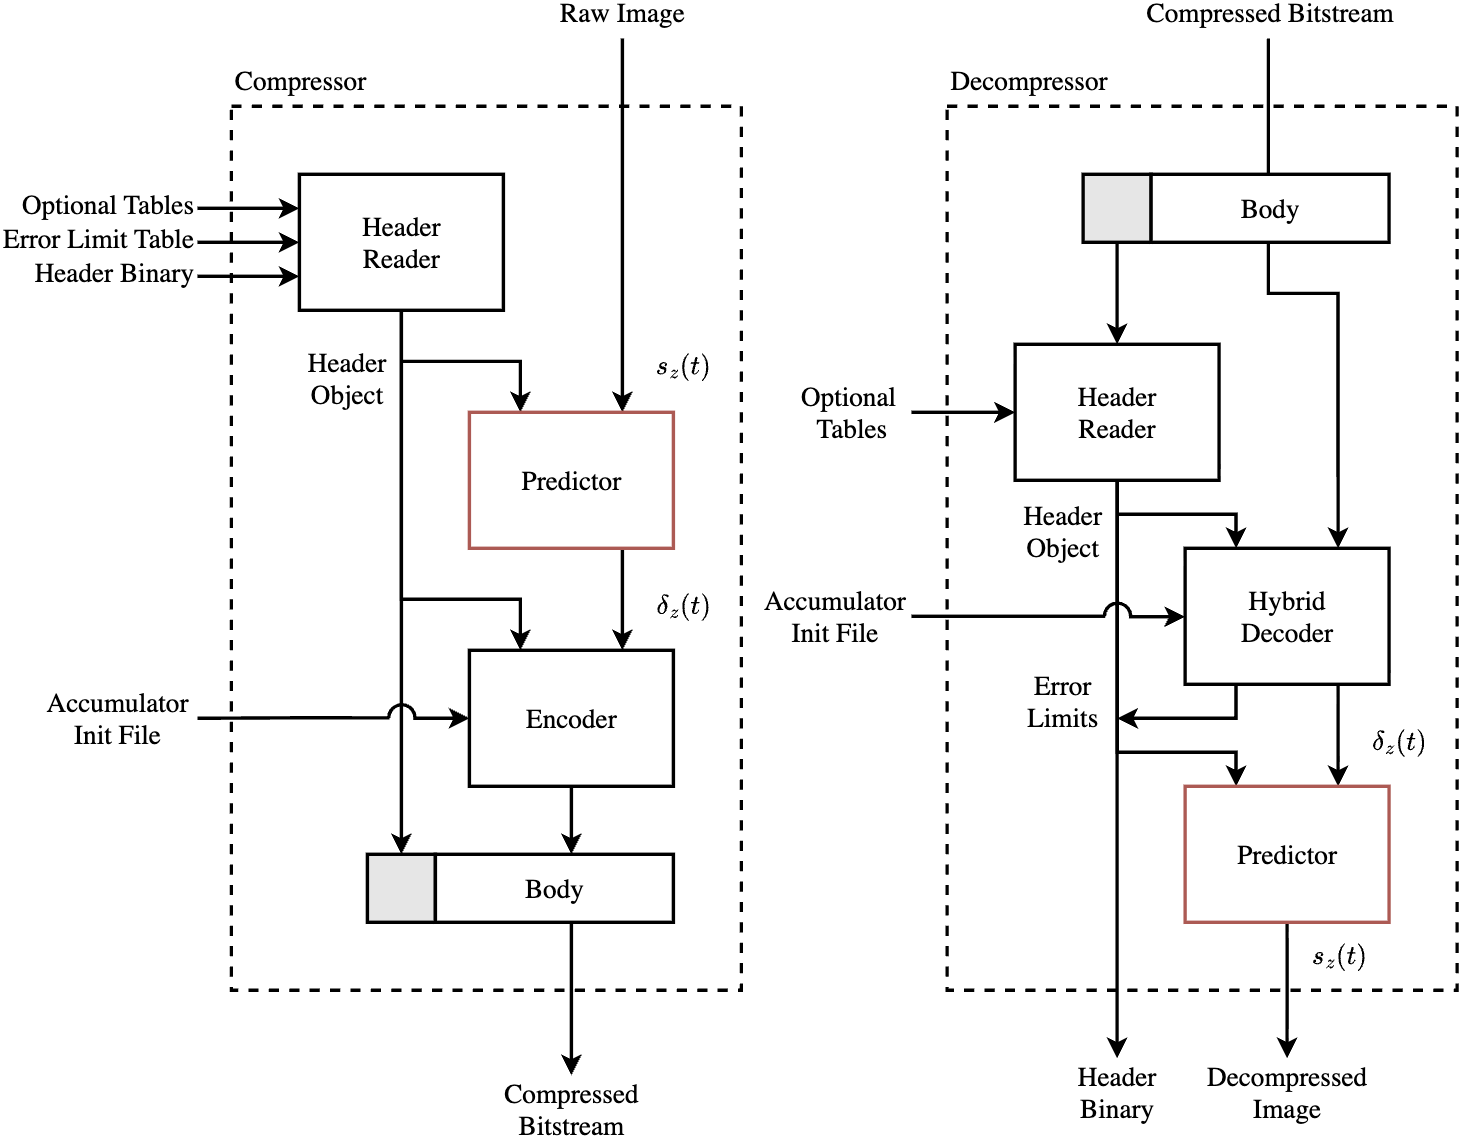
\includegraphics[width=1\textwidth]{figures/verification-model.png}
	\end{center}
	\caption{}
	\label{fig:verification-model}
\end{figure}


% Predictor with compression and decompression implementation in C++. Pybind11, integration with build system. PiP, scikit, Numpy arrays in cpp. Memory ordering and quick access to arrays. Life of allocated memory.
%
% Reconstruction of mapped quantizer indices from compressed bitstream, hybrid encoder.
%
% Header reader used for reading header config from compressed bitstream.
%
% When decoding, also read encoded error limits and set in header class. Output as file in the end.
%
% Note on predictor data types
%
% When storing final, decompressed image make sure to store in correct ordering.
%
% Sampler class.
%
% Construction of verification data: using CNES decompressor with test vector set.
%
% Bitarray module for python.
%
% Rounding bit added to bitstream to allow reconstruction of average estimate model.
%
% Debugging framework, reference file. Debugging flow?

\begin{lstlisting}[
    float=ht,
    caption={Pseudocode for hybrid decoder.},
    label=lst:pseudocode,
    language=Python]
accumulator, active_prefixes = decode_image_tail()
counter                      = get_counter_value(t_max)

for all z and t: # iterate in reverse order
    mapped_quantizer_index[z, t] = decode_sample(z, t)
    if ordering = BI and prediodic_error_limit_updating:
        header.error_limits[z] = decode_error_limts(z)

def decode_sample(z, t): # pops bits from compressed bitstream
    if t = 0: # first sample encoded as is
        mapped_quantizer_index[z, t] = read_D_bit_integer()
    else:
        if accumulator[z, t] * 2^14 >= threshold[0] * counter[t]:
            mapped_quantizer_index[z, t] = decode_high_entropy(z, t)
        else:
            mapped_quantizer_index[z, t] = decode_low_entropy(z, t)

    t_next = t-1
    counter[t_next] = get_counter_value(t_next)

    # update accumulator
    if counter[t_next] = 2^rescaling_counter_size - 1: # rescaling
        rounding_bit = bitstream.pop()
        updated_accumulator = 2 * accumulator[z, t] - 4 * mapped_quantizer_index[z, t] - 1

        if rounding_bit = 0 and updated_accumulator_lsb = 1:
            updated_accumulator += 1 # ensure even
        else if rounding_bit = 1 and updated_accumulator_lsb = 0:
            updated_accumulator += 1 # ensure odd
        accumulator[z, t_next] = updated_accumulator

    else: # normal case
        accumulator[z, t_next] = accumulator[z, t] - 4 * mapped_quantizer_index[z, t]
\end{lstlisting}

\section{Hardware Modifications}

\begin{figure}[ht]
	\begin{center}
		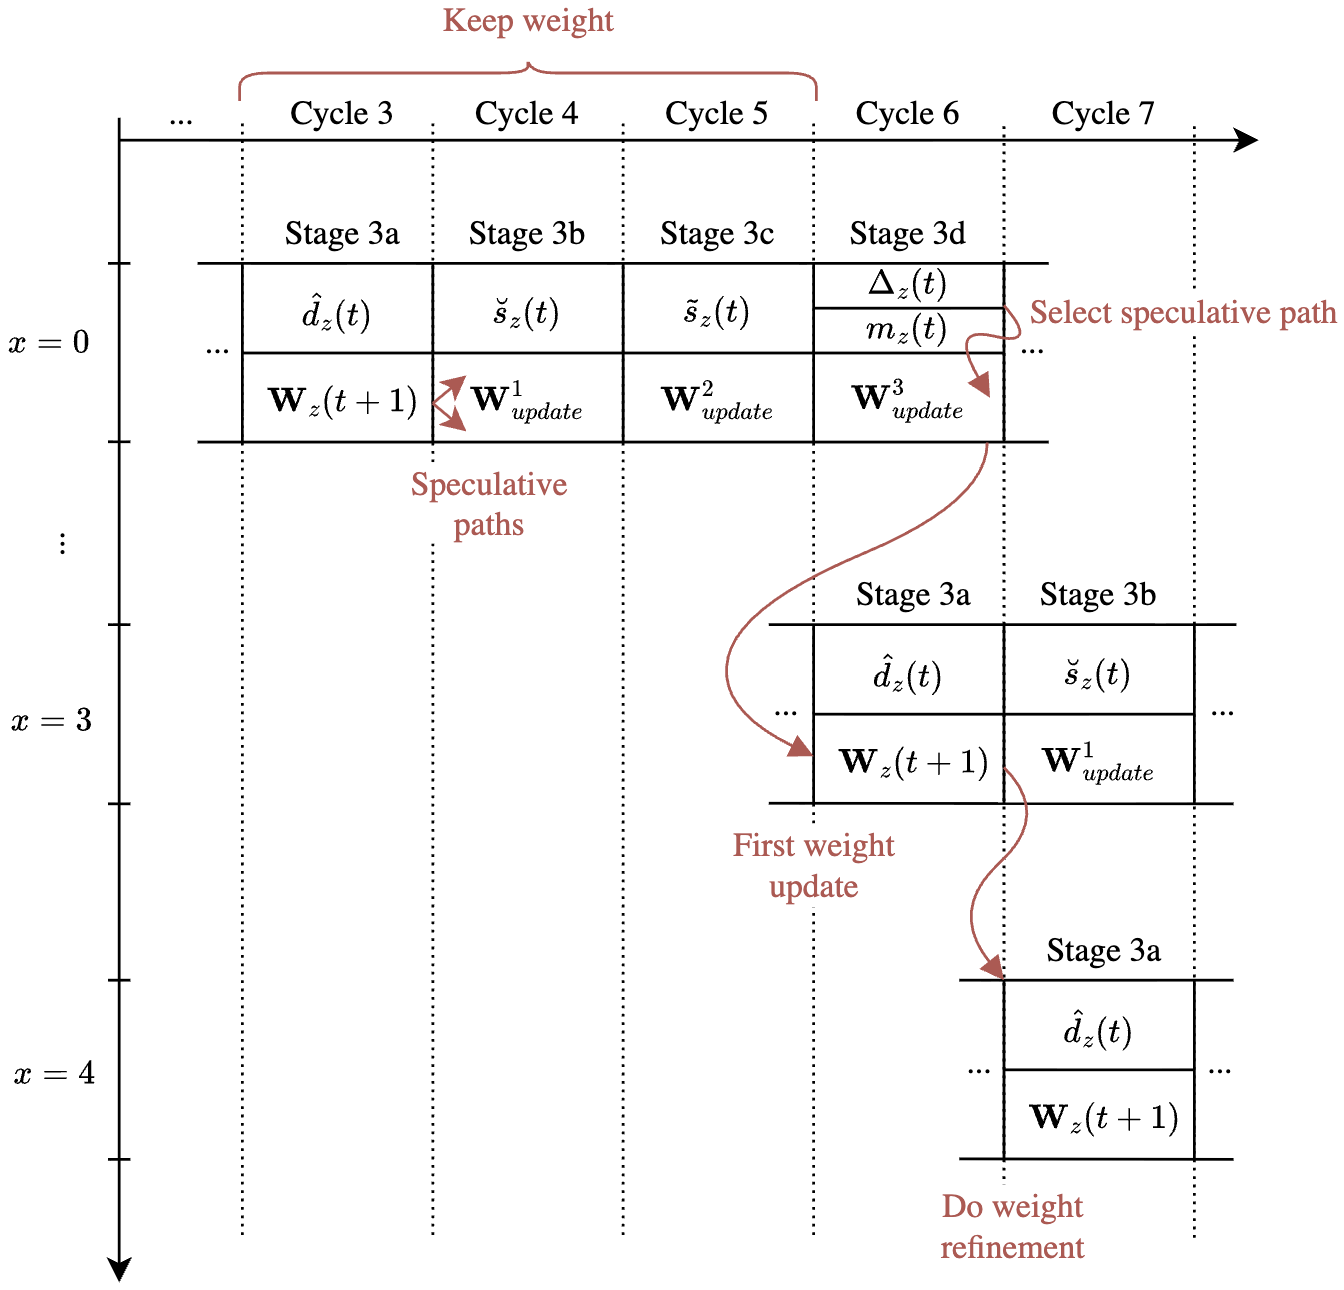
\includegraphics[width=0.85\textwidth]{figures/new-stage3.png}
	\end{center}
	\caption{Proposed pipeline for delayed weight updates.}
	\label{fig:new-stage3}
\end{figure}

\begin{figure}[ht]
	\begin{center}
		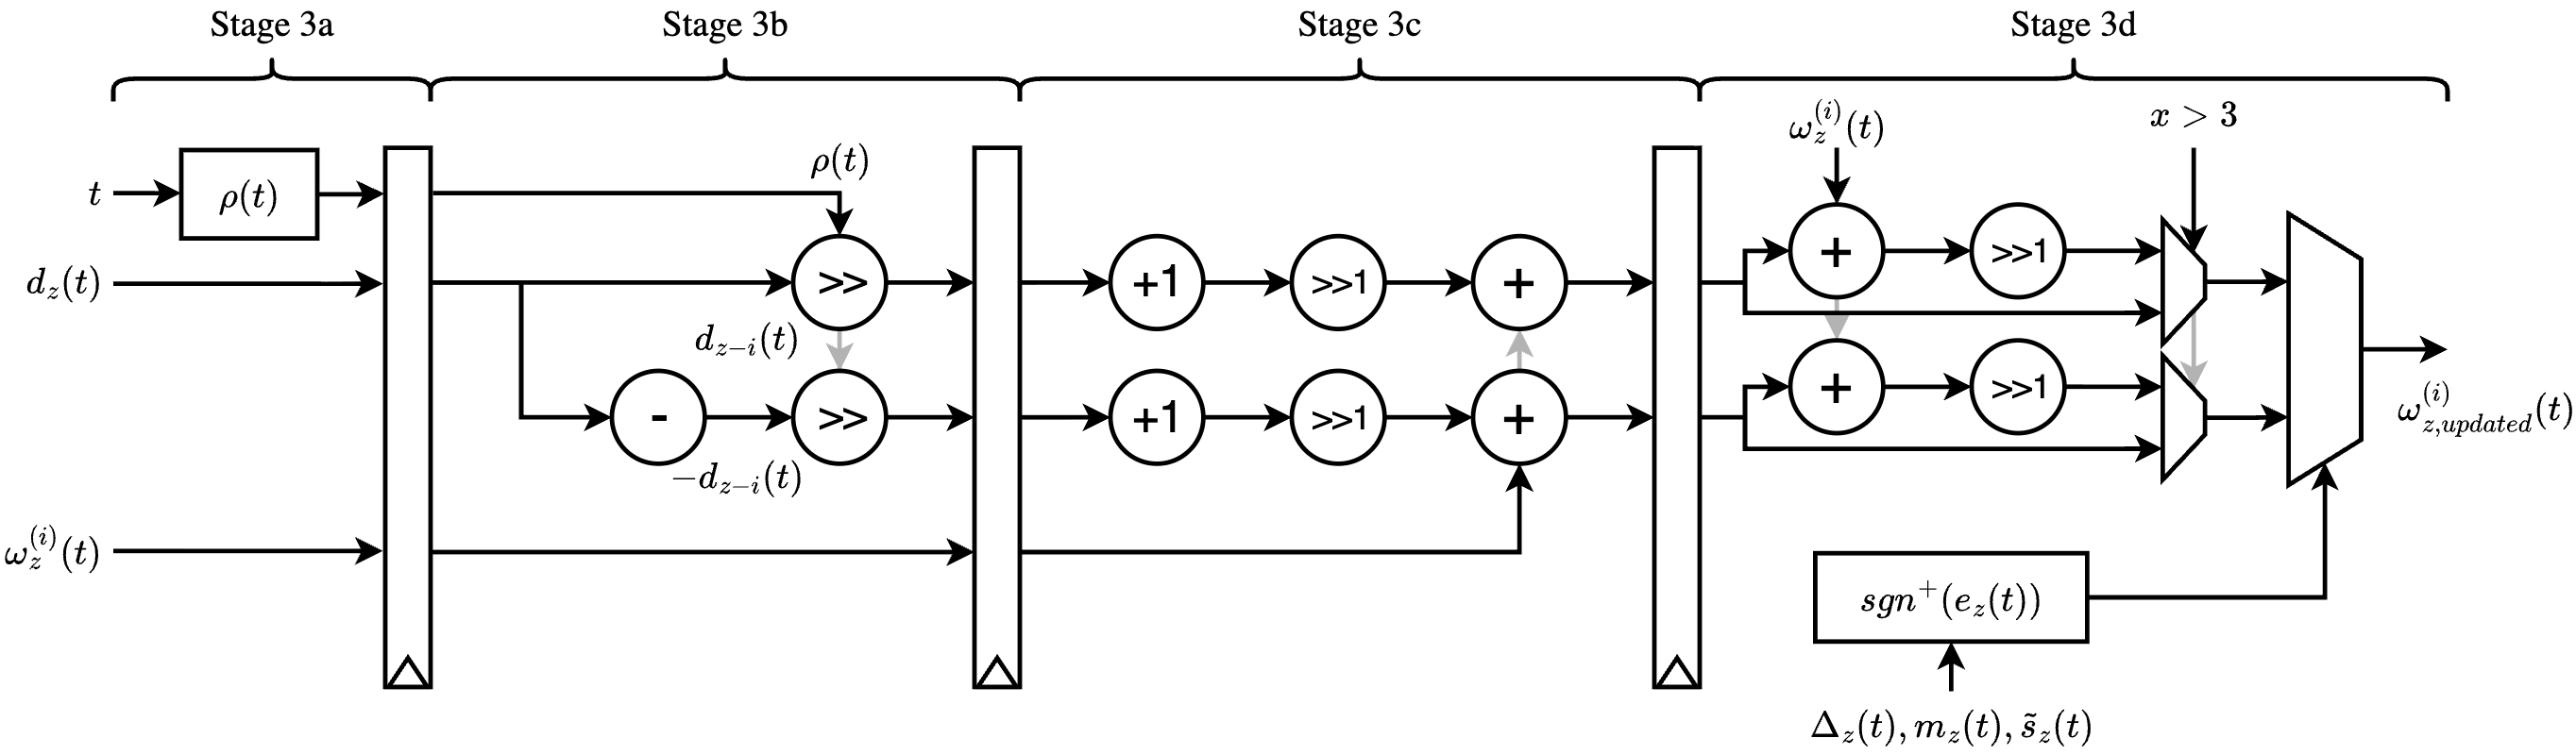
\includegraphics[width=1\textwidth]{figures/weights-pipeline-hw.png}
	\end{center}
	\caption{}
	\label{fig:weights-pipeline-hw}
\end{figure}

\begin{figure}[ht]
	\begin{center}
		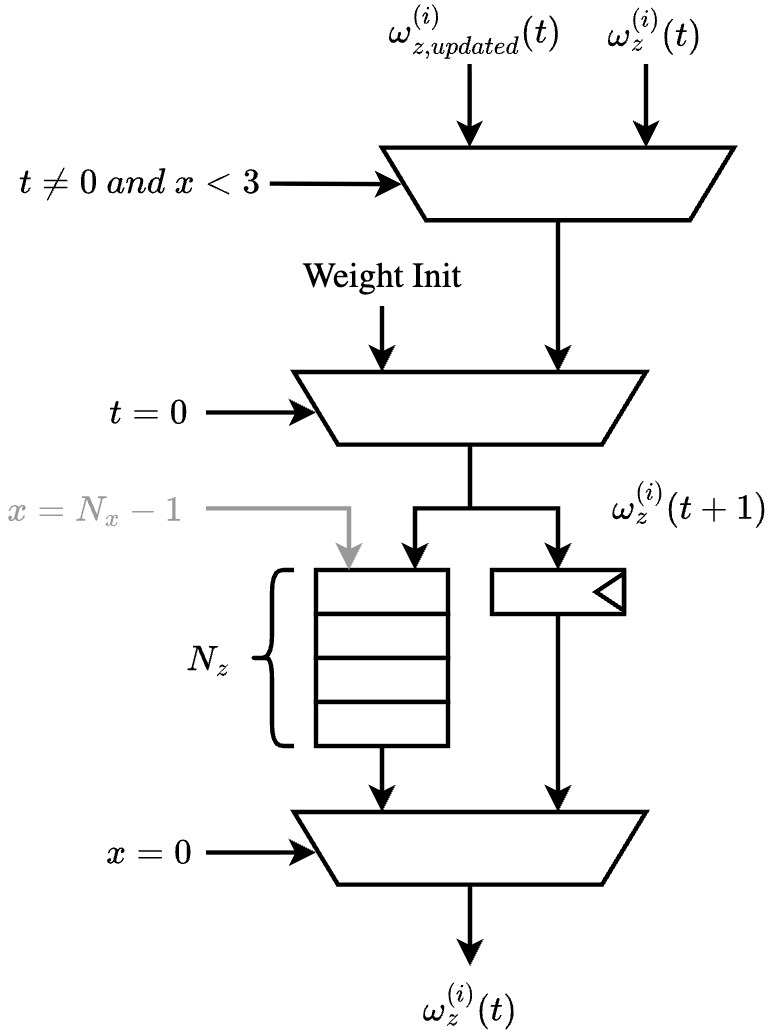
\includegraphics[width=0.45\textwidth]{figures/weights-hw.png}
	\end{center}
	\caption{}
	\label{fig:weights-hw}
\end{figure}

% Analysis of the new critical path after implementation of the new weight update scheme showed that the new path was in the sample representative stage

\begin{figure}[ht]
	\begin{center}
		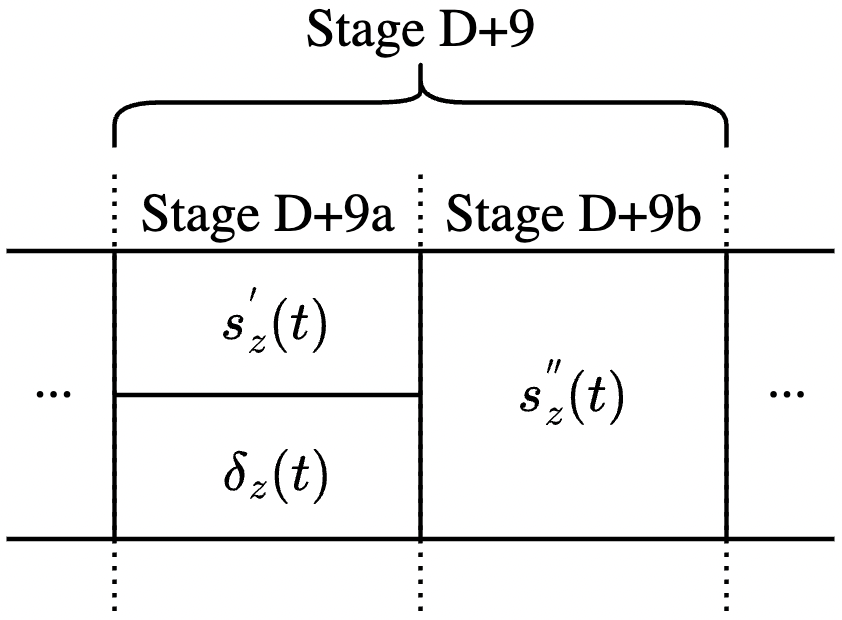
\includegraphics[width=0.3\textwidth]{figures/new-stageD9.png}
	\end{center}
	\caption{Sample representative stage split into two stages $D+9a$ and $D+9b$, reducing the new critical path after splitting the weight update stage.}
	\label{fig:new-stageD9}
\end{figure}

\begin{figure}[ht]
	\begin{center}
		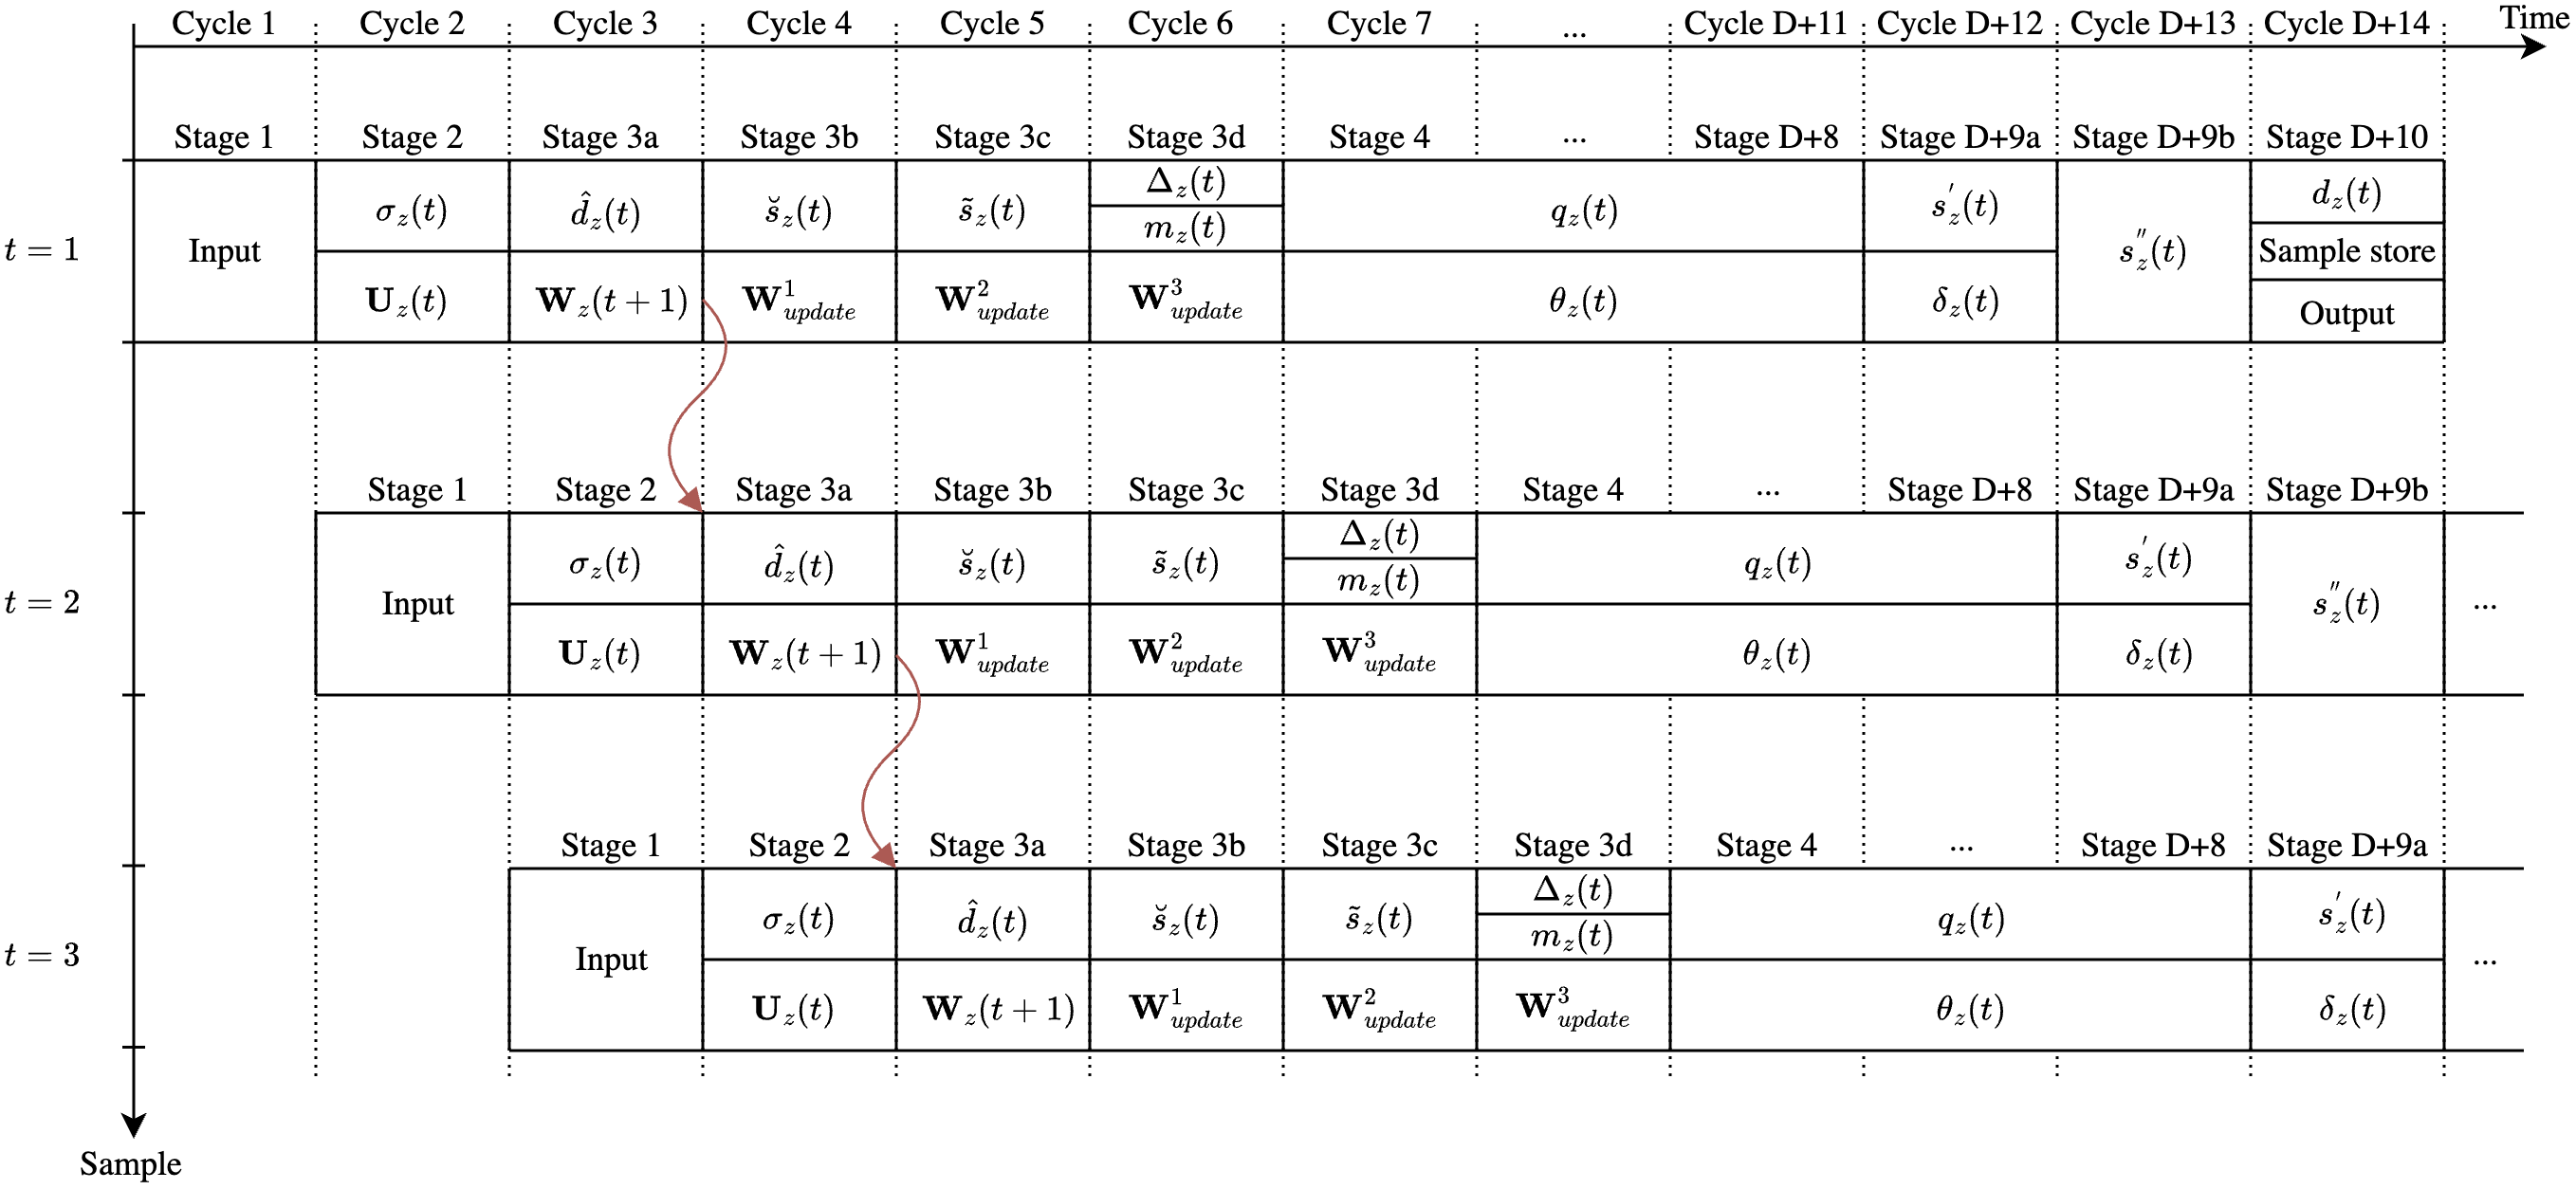
\includegraphics[angle=90, height=1\textheight]{figures/new-pipeline.png}
	\end{center}
	\caption{Proposed pipeline with delayed weight updates allowing splitting stage 3 into four separate stages, 3a to 3d. Additionally, the sample representative calculation in stage $D+9$ is split into two stages $D+9a$ and $D+9b$.}
	\label{fig:new-pipeline}
\end{figure}

\section{Hardware Verification}

\section{Hardware Testing}

\begin{table}[ht]
	\centering
	\caption{Selected predictor and hybrid encoder parameters. Values are selected based on the work by \citeauthor{blanesPerformanceImpactParameter2019}, and are the same as those used by \citeauthor{vorhaugHyperspectralImageCompression2024} \cite{blanesPerformanceImpactParameter2019, vorhaugHyperspectralImageCompression2024}. Table recreated from \cite{vorhaugHyperspectralImageCompression2024}.}
	\label{tab:parameters}
	\begin{tabular}{lcl}
		\toprule
		\textbf{Name}                    & \textbf{Symbol}              & \textbf{Configuration} \\
		\midrule
		Sample type                      &                              & Unsigned               \\
		Dynamic range                    & $D$                          & 16                     \\
		Sample encoding order            &                              & BIL                    \\
		Entropy coder type               &                              & Hybrid coder           \\
		Quantizer method                 &                              & Absolute               \\
		Number of prediction bands       & $P$                          & 3                      \\
		Register size                    & $R$                          & 64                     \\
		Local sum type                   &                              & Narrow column-oriented \\
		Prediction mode                  &                              & Reduced                \\
		Weight component resolution      & $\Omega$                     & 19                     \\
		Weight initialization method     &                              & Default                \\
		Weight update initial parameter  & $\nu_{\min}$                 & $-1$                   \\
		Weight update final parameter    & $\nu_{\max}$                 & $4$                    \\
		Weight update change interval    & $t_{\text{inc}}$             & $2^6$                  \\
		Weight update exponent offsets   & $\zeta_z^{(i)}, \zeta_z^{*}$ & $0$                    \\
		Periodic error limit update      &                              & Disabled               \\
		Band-varying absolute limits     &                              & Disabled               \\
		Absolute error limit             & $a_z$                        & \emph{Varied}          \\
		Band-varying relative limits     &                              & Disabled               \\
		Relative error limit             & $r_z$                        & $0$                    \\
		Sample representative resolution & $\Theta$                     & $3$                    \\
		Sample representative offset     & $\psi_z$                     & $7$                    \\
		Band-varying offset              &                              & Disabled               \\
		Sample representative damping    & $\theta_z$                   & $3$                    \\
		Band-varying damping             &                              & Disabled               \\
		Unary length limit               & $U_{\max}$                   & $18$                   \\
		Rescaling counter size           & $\gamma^{*}$                 & $6$                    \\
		Initial count exponent           & $\gamma_0$                   & $1$                    \\
		Accumulator initialization value & $\tilde{\Sigma}_z(0)$        & $4 \cdot 2^{\gamma_0}$ \\
		\bottomrule
	\end{tabular}
\end{table}

\chapter{Results}
\label{sec:results}

The following sections present results from analysis of the verification model, compression performance of the delayed weight update scheme, and performance of the modified hardware design. The \acrshort{hypso}-2 coastline image set is presented in \autoref{app:coastline-images}, consisting of ten images. The images have dimensions $N_z=120$, $N_y=598$ and $N_x=1092$, for a total of $78.36$ million samples, taken at a frame rate of $8$ frames per second. Images from the AVIRIS Yellowstone set have dimensions of $N_z=224$, $N_y=512$, and varying size in the $x$ dimension of $N_x \in \{614, 677, 680\}$, for roughly $77$ million samples.

\section{Verification Model}

\begin{figure}[ht]
	\begin{center}
		\efbox{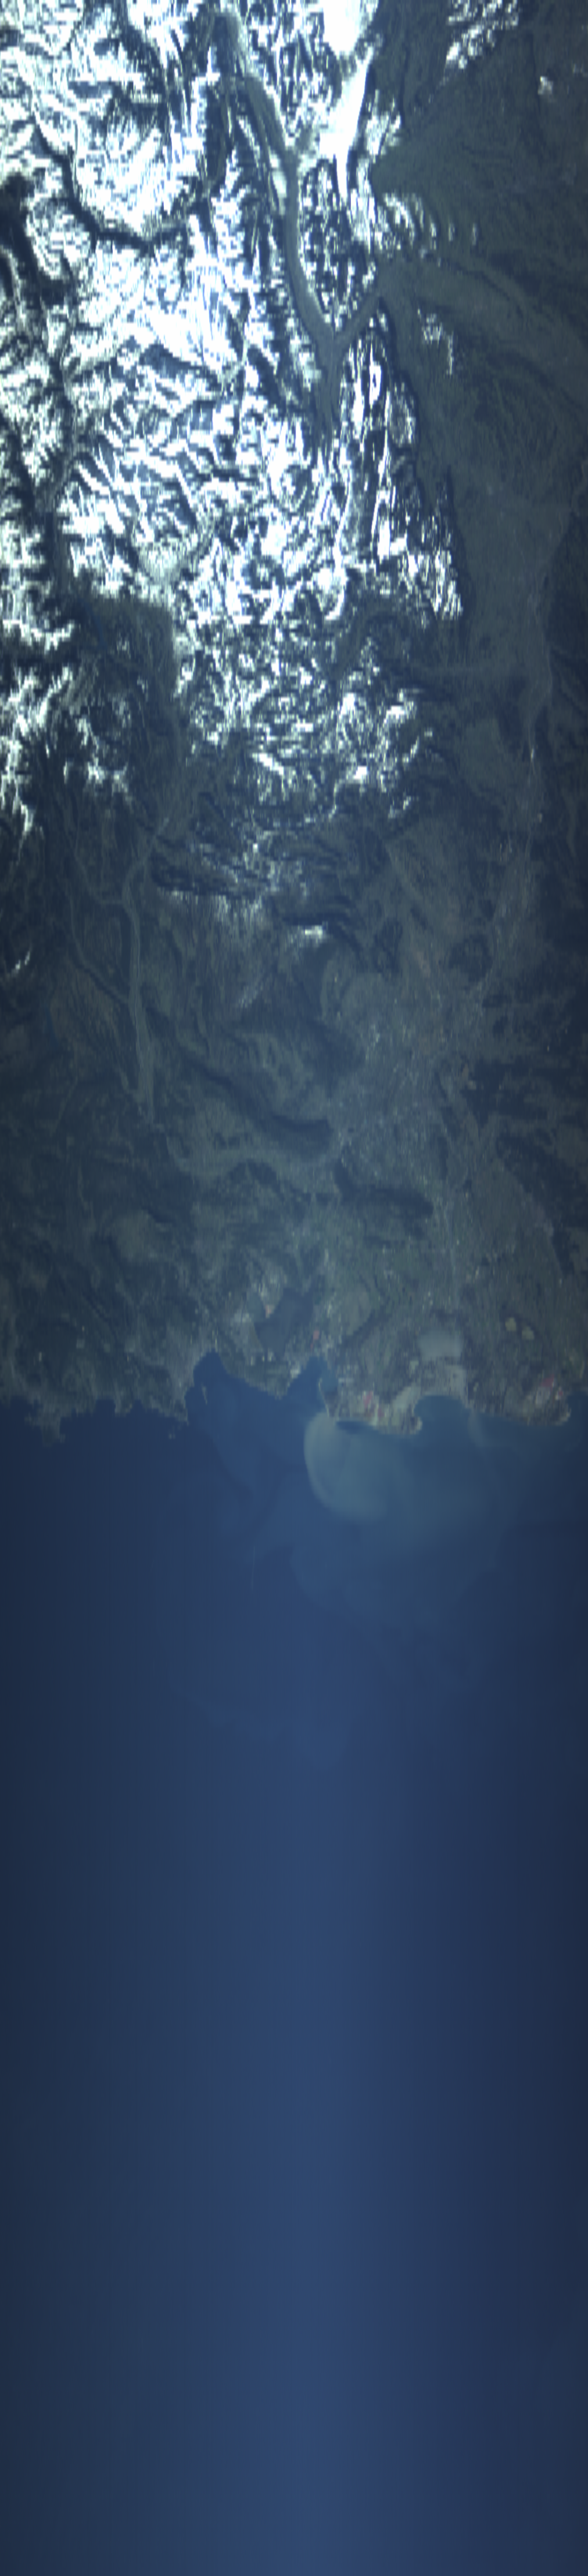
\includegraphics[height=0.28\textheight,valign=t]{figures/hypso2-rgb/hypso_decoded.png}}
		\efbox{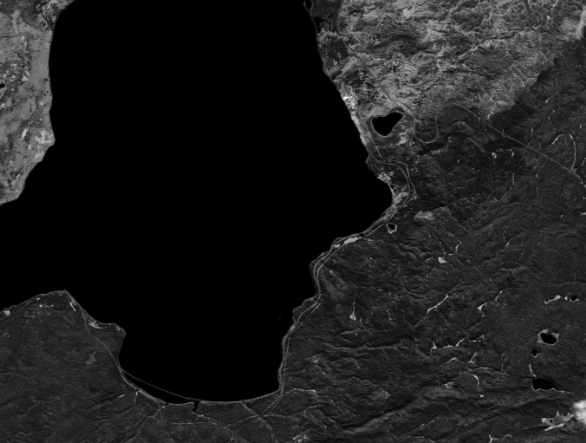
\includegraphics[height=0.28\textheight,valign=t]{results/aviris/aviris_decoded.png}}
		% 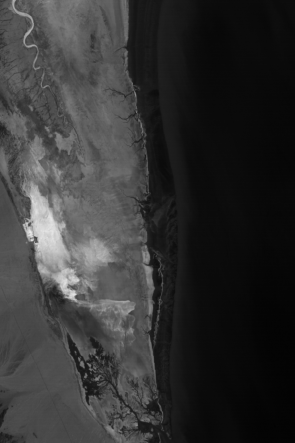
\includegraphics[height=0.28\textheight,valign=t]{results/landsat/landsat_decoded.png}
	\end{center}
	\caption{Two decompressed images from HYPSO-2 and AVIRIS Yellowstone, compressed with delayed weight update scheme with $r_z=16$ and $a_z=4$.}
	\label{fig:decompressed}
\end{figure}

\autoref{fig:decompressed} shows two images from the \acrshort{hypso}-2 coastline and AVIRIS Yellowstone sets that have been compressed and decompressed using the verification model, with delayed weight updates. The images were compressed using $r_z=16$ and $a_z=4$, giving compression ratios of $2.47$ and $4.31$ for HYPSO-2 and AVIRIS images respectively. Visual inspection shows that the verification model can successfully reconstruct the original images, while employing the modified weight update scheme. Additionally, all images from both image sets have been compressed in lossless mode, in which all reconstructed images are identical to the originals.

\begin{figure}[ht]
	\begin{center}
		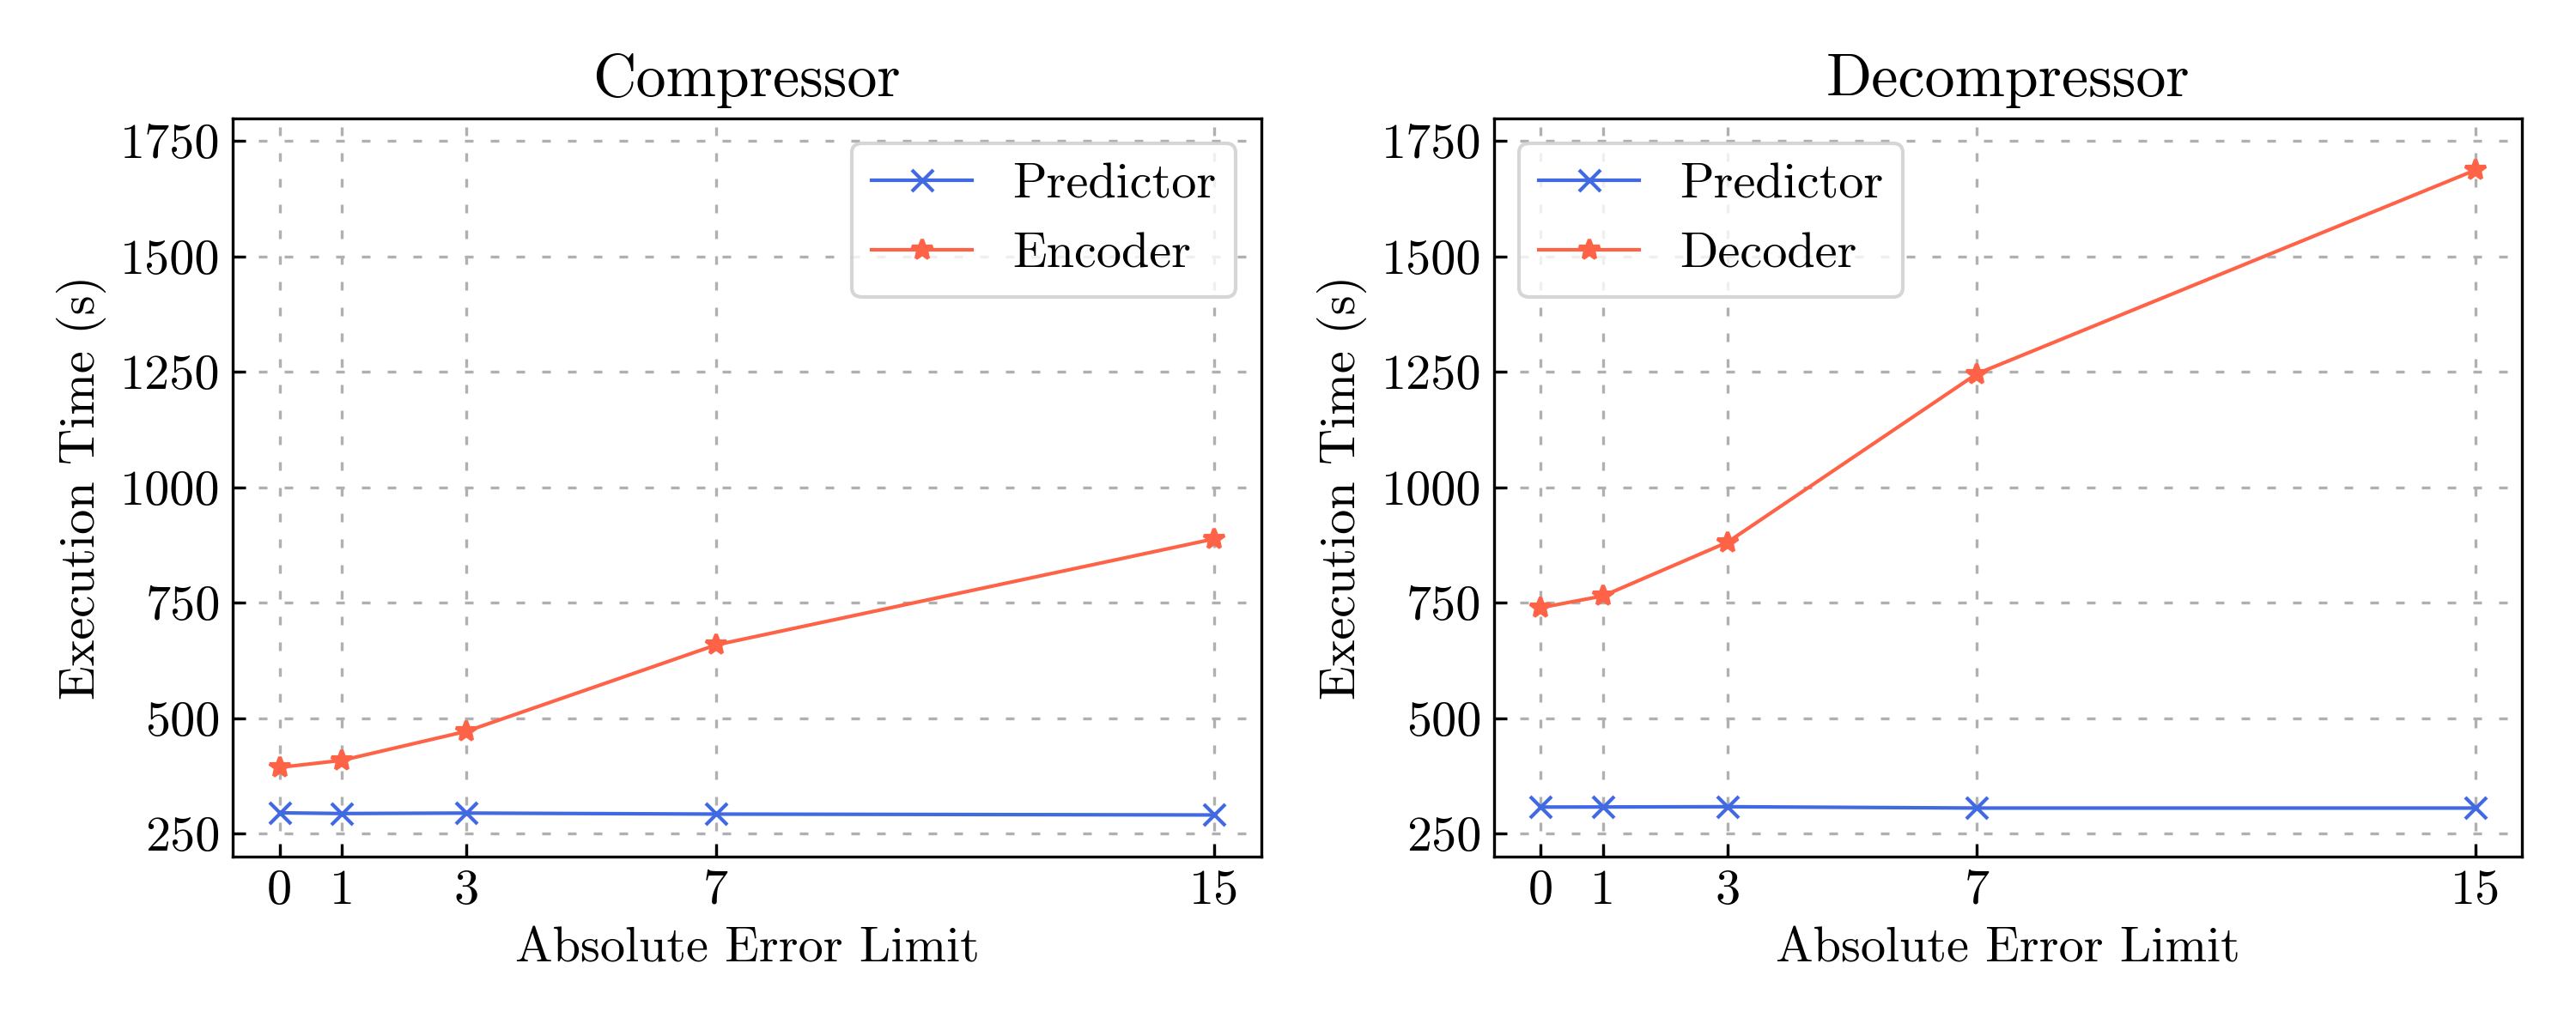
\includegraphics[width=1\textwidth]{figures/execution_time.png}
	\end{center}
	\caption{Execution time for the C++ predictor and hybrid encoder modules during compression and decompression for a set of absolute error limits. Results are averaged over a set of ten \acrshort{hypso}-2 images.}
	\label{fig:execution_time}
\end{figure}

Execution time of the verification model is analysed using the \acrshort{hypso}-2 coastline set, and is averaged across the images for a set of \acrshort{PAE}s. The four main stages of compression/decompression are timed separately: load data, predictor, encoder/decoder, and save data. Tests are run on a computer with an AMD Ryzen 5 3600X CPU and 64 GB of RAM. Tables \ref{tab:coastline-compress} and \ref{tab:coastline-decompress} summarize the execution time results for compression and decompression using the verification model. The same results are visualized in \autoref{fig:execution_time}.

Execution time of the C++ predictor remains more or less constant at $~300$ seconds for both compression and decompression. The hybrid encoder, still written in Python, displays a significant increase in execution time as the absolute error limit is adjusted. This change is most prominent in the decoder stage of the decompressor, with execution times almost double those of the encoder stage of the compressor. The increasing execution times are likely due to the use of \acrshort{V2V} codes as predicted sample entropy decreases for higher absolute error limits.

During compression, execution time for the loading and saving of data to and from the disk is negligible. For the decompressor, saving data takes $~70$ seconds. This is because all image samples must be iterated over and stored to file in the correct sample store order (\acrshort{BIL}, \acrshort{BIP}, \acrshort{BSQ}), as dictated by the header configuration. The compressor can store the compressed bitstream directly to file without modifications.

\autoref{tab:coastline-compress-py} shows execution times for compression using the old predictor module written in Python. The predictor has a runtime of $~2100$ seconds, over seven times slower than that of the C++ predictor. Saving output data also takes significantly longer. This is because the module stores additional, intermediate results, a feature that is made optional in the C++ predictor.

\begin{table}[ht]
	\caption{Performance of compression using verification model with C++ predictor and delayed weight updates averaged over ten HYPSO-2 images for a set of PAEs.}
	\label{tab:coastline-compress}
	\begin{center}
		\begin{tabular}{lrrrrrr}
			\hline
			\textbf{PAE} & \textbf{CR} & \textbf{Load Data (s)} & \textbf{Predictor (s)} & \textbf{Encoder (s)} & \textbf{Save Data (s)} & \textbf{Total (s)} \\
			\hline
			% 0            & 1.995       & 0.311                  & 295.273                & 393.706              & 0.069                  &                    \\
			% 1            & 2.488       & 0.121                  & 293.722                & 408.911              & 0.054                  &                    \\
			% 3            & 3.077       & 0.076                  & 294.704                & 471.881              & 0.044                  &                    \\
			% 7            & 3.912       & 0.076                  & 292.520                & 658.729              & 0.034                  &                    \\
			% 15           & 5.219       & 0.076                  & 290.610                & 888.570              & 0.024                  &                    \\
			0            & 1.995       & 0.311                  & 295.273                & 393.706              & 0.069                  & 691.354            \\
			1            & 2.488       & 0.121                  & 293.722                & 408.911              & 0.054                  & 705.296            \\
			3            & 3.077       & 0.076                  & 294.704                & 471.881              & 0.044                  & 769.782            \\
			7            & 3.912       & 0.076                  & 292.520                & 658.729              & 0.034                  & 955.271            \\
			15           & 5.219       & 0.076                  & 290.610                & 888.570              & 0.024                  & 1184.499           \\
			\hline
		\end{tabular}
	\end{center}
\end{table}

\begin{table}[ht]
	\caption{Performance of decompression using verification model with C++ predictor and delayed weight updates averaged over ten HYPSO-2 images for a set of PAEs.}
	\label{tab:coastline-decompress}
	\begin{center}
		\begin{tabular}{lrrrrrr}
			\hline
			\textbf{PAE} & \textbf{Load Data (s)} & \textbf{Decoder (s)} & \textbf{Predictor (s)} & \textbf{Save Data (s)} & \textbf{Total (s)} \\
			\hline
			% 0            & 0.528                  & 739.573              & 307.741                & 70.009                 &                    \\
			% 1            & 0.439                  & 764.869              & 307.902                & 71.326                 &                    \\
			% 3            & 0.347                  & 881.335              & 308.484                & 70.614                 &                    \\
			% 7            & 0.229                  & 1245.921             & 305.587                & 70.191                 &                    \\
			% 15           & 0.112                  & 1687.085             & 305.571                & 69.964                 &                    \\
			0            & 0.528                  & 739.573              & 307.741                & 70.009                 & 1117.851           \\
			1            & 0.439                  & 764.869              & 307.902                & 71.326                 & 1144.536           \\
			3            & 0.347                  & 881.335              & 308.484                & 70.614                 & 1260.780           \\
			7            & 0.229                  & 1245.921             & 305.587                & 70.191                 & 1621.928           \\
			15           & 0.112                  & 1687.085             & 305.571                & 69.964                 & 2062.732           \\
			\hline
		\end{tabular}
	\end{center}
\end{table}

\begin{table}[ht]
	\caption{Performance of compression using verification model with Python predictor and delayed weight updates averaged over ten HYPSO-2 images for a set of PAEs. \textbf{TODO} update values when results are ready.}
	\label{tab:coastline-compress-py}
	\begin{center}
		\begin{tabular}{lrrrrrr}
			\hline
			\textbf{PAE} & \textbf{CR} & \textbf{Load Data (s)} & \textbf{Predictor (s)} & \textbf{Encoder (s)} & \textbf{Save Data (s)} & \textbf{Total (s)} \\
			\hline
			% 0            & 1.923       & 0.339                  & 2091.803               & 391.609              & 244.665                &                    \\
			% 1            & 2.378       & 0.600                  & 2117.772               & 400.696              & 247.626                &                    \\
			% 3            & 2.905       & 0.290                  & 2117.119               & 412.869              & 245.374                &                    \\
			% 7            & 3.636       & 0.075                  & 2115.089               & 527.766              & 245.211                &                    \\
			% 15           & 4.798       & 0.081                  & 2132.114               & 880.100              & 243.001                &                    \\
			0            & 1.923       & 0.339                  & 2091.803               & 391.609              & 244.665                & 2730.339           \\
			1            & 2.378       & 0.600                  & 2117.772               & 400.696              & 247.626                & 2769.072           \\
			3            & 2.905       & 0.290                  & 2117.119               & 412.869              & 245.374                & 2778.557           \\
			7            & 3.636       & 0.075                  & 2115.089               & 527.766              & 245.211                & 2891.777           \\
			15           & 4.798       & 0.081                  & 2132.114               & 880.100              & 243.001                & 3260.094           \\
			\hline
		\end{tabular}
	\end{center}
\end{table}

\section{Compression Performance}

The compression performance with and without delayed weight updates is averaged over the \acrshort{hypso}-2 coastline and AVIRIS Yellowstone image sets for a set of \acrshort{PAE}s. Tests are performed using the verification model for compression with delayed weight updates, and the \acrshort{CNES} compression tool for issue 2 standard compliant tests. Results are presented in figures \ref{fig:compression-performance-hypso} and \ref{fig:compression-performance-aviris}, and are given as bits per sample and compression ratio. As expected, compression performance improves as the absolute error limit increases. Images from the AVIRIS Yellowstone set achieve significantly higher compression performance than \acrshort{hypso}-2, reaching the sub-1 bits per sample threshold at $a_z=15$. This shows that image samples of of AVIRIS image sensor display higher correlation than those of the \acrshort{hypso}-2 image sensor, and thus are better suited for predictive compression such as the issue 2 algorithm.

\begin{table}[ht]
	\caption{Reduction in compression ratio using the delayed weight update scheme for a set of absolute errors.}
	\label{tab:coastline-reduction}
	\begin{center}
		\begin{tabular}{lcc}
			\hline
			\textbf{PAE} & \textbf{HYPSO-2, coastline} & \textbf{AVIRIS, Yellowstone} \\
			\hline
			0            & $-0.371\%$                  & $-2.711\%$                   \\
			1            & $-0.470\%$                  & $-4.534\%$                   \\
			3            & $-0.565\%$                  & $-4.898\%$                   \\
			7            & $-0.739\%$                  & $-4.872\%$                   \\
			15           & $-0.826\%$                  & $-4.484\%$                   \\
			\hline
		\end{tabular}
	\end{center}
\end{table}

\autoref{tab:coastline-reduction} summarizes the reduction in compression performance due to delayed weight updates for the two image sets. Reduction increases slightly for higher \acrshort{PAE}s, and is overall higher for the AVIRIS Yellowstone images. Higher correlation between image samples can mean that the compression is more sensitive to the quality of the weight vectors, resulting in a higher compression penalty. \acrshort{hypso}-2 coastline images show a reduction of less than $1\%$ for the selected \acrshort{PAE}s. These results show that the applicable image sensor is a key factor for deciding the plausability of using the delayed weight update scheme.

\begin{figure}[ht]
	\begin{center}
		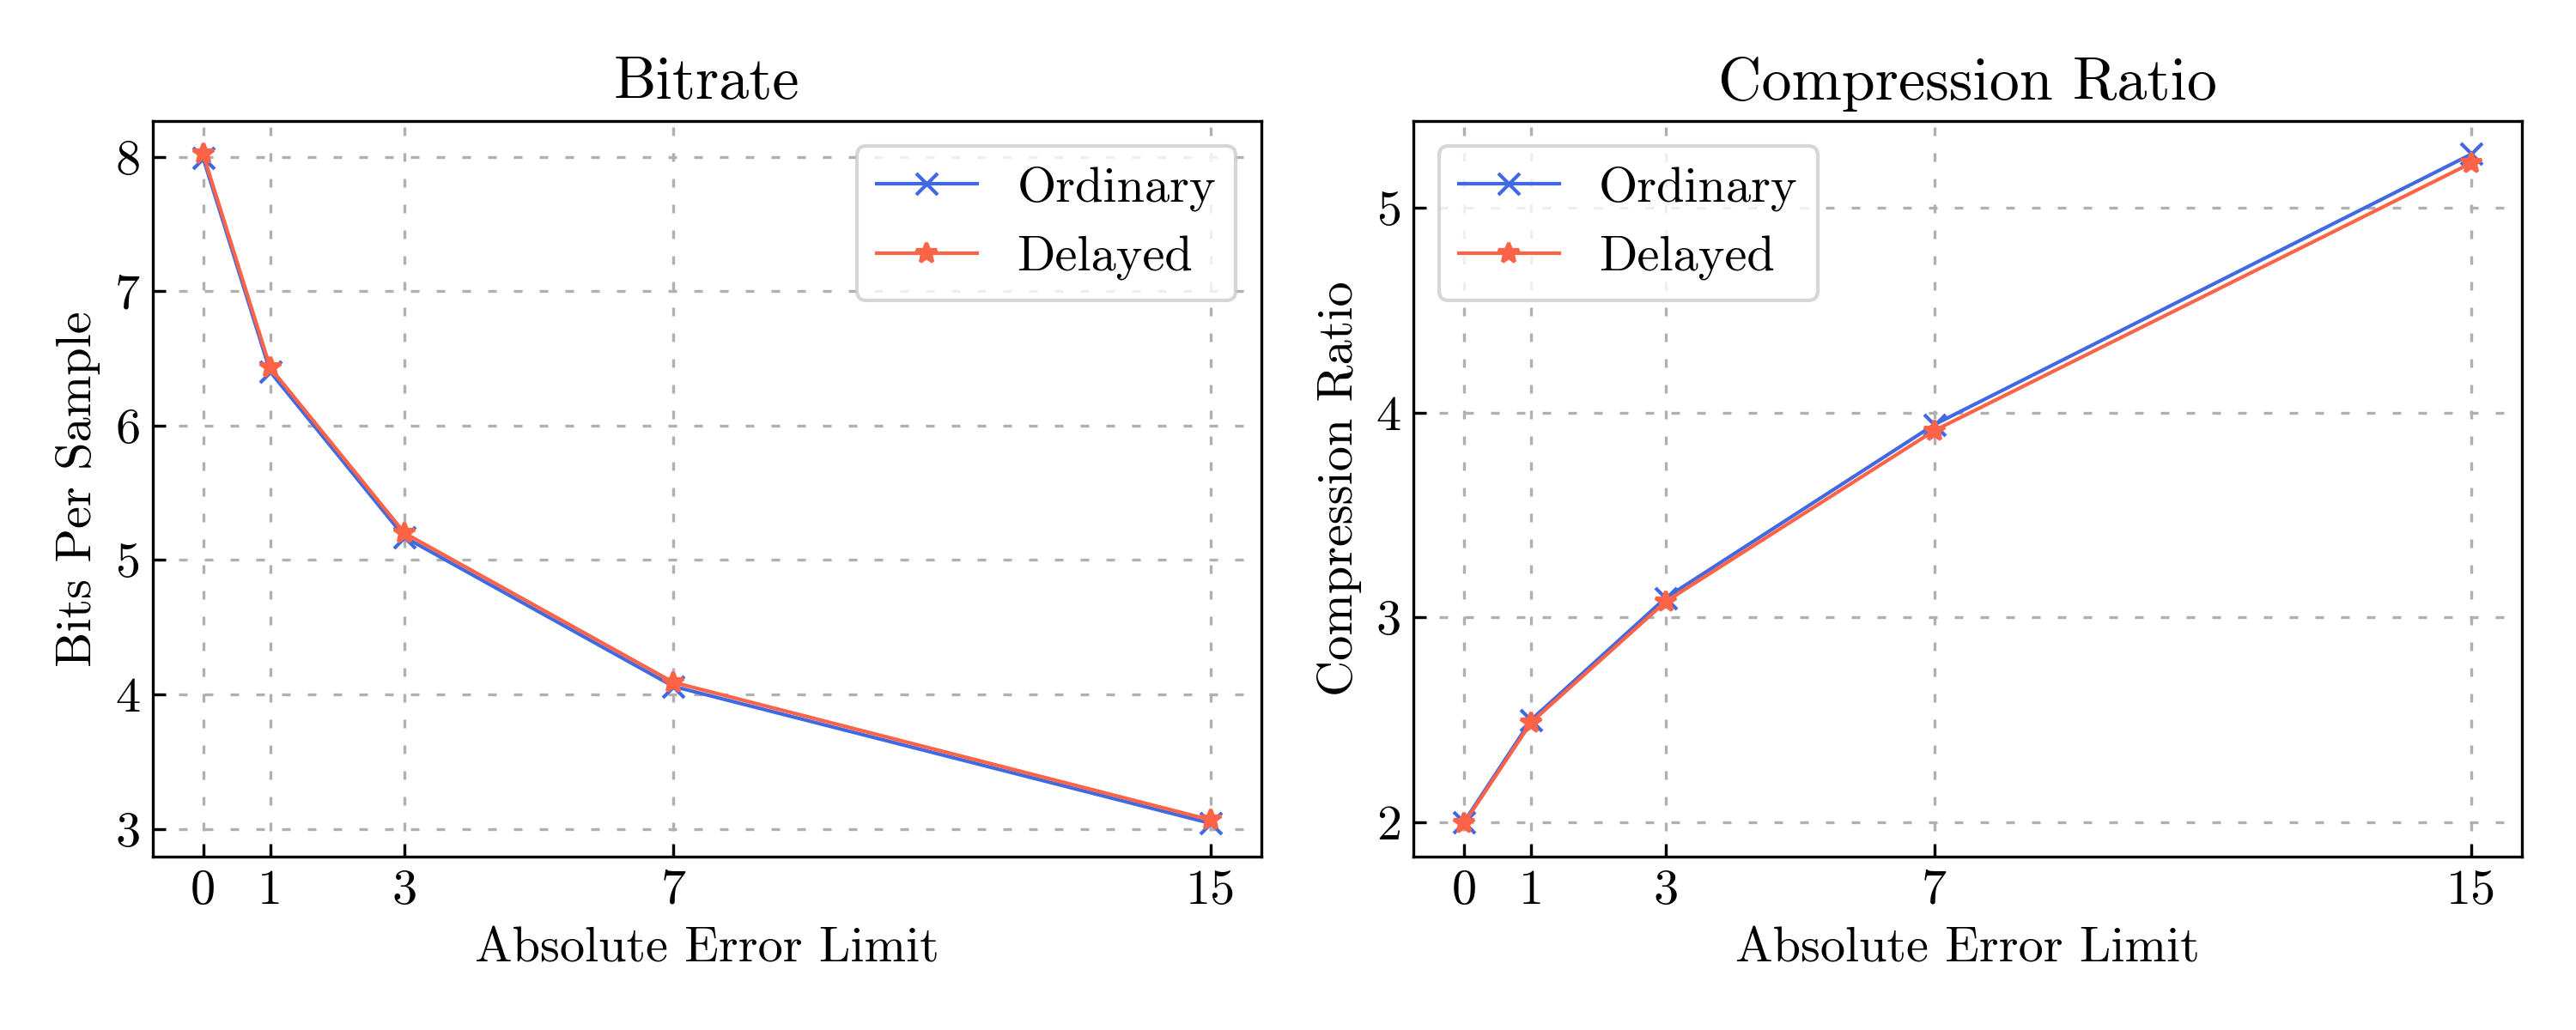
\includegraphics[width=1\textwidth]{figures/compression_performance_hypso.png}
	\end{center}
	\caption{Compression performance presented in bits per sample and compression ratio for a set of absolute error limits. Results are averaged over a set of ten \acrshort{hypso}-2 coastline images with $D=16$.}
	\label{fig:compression-performance-hypso}
\end{figure}

\begin{figure}[ht]
	\begin{center}
		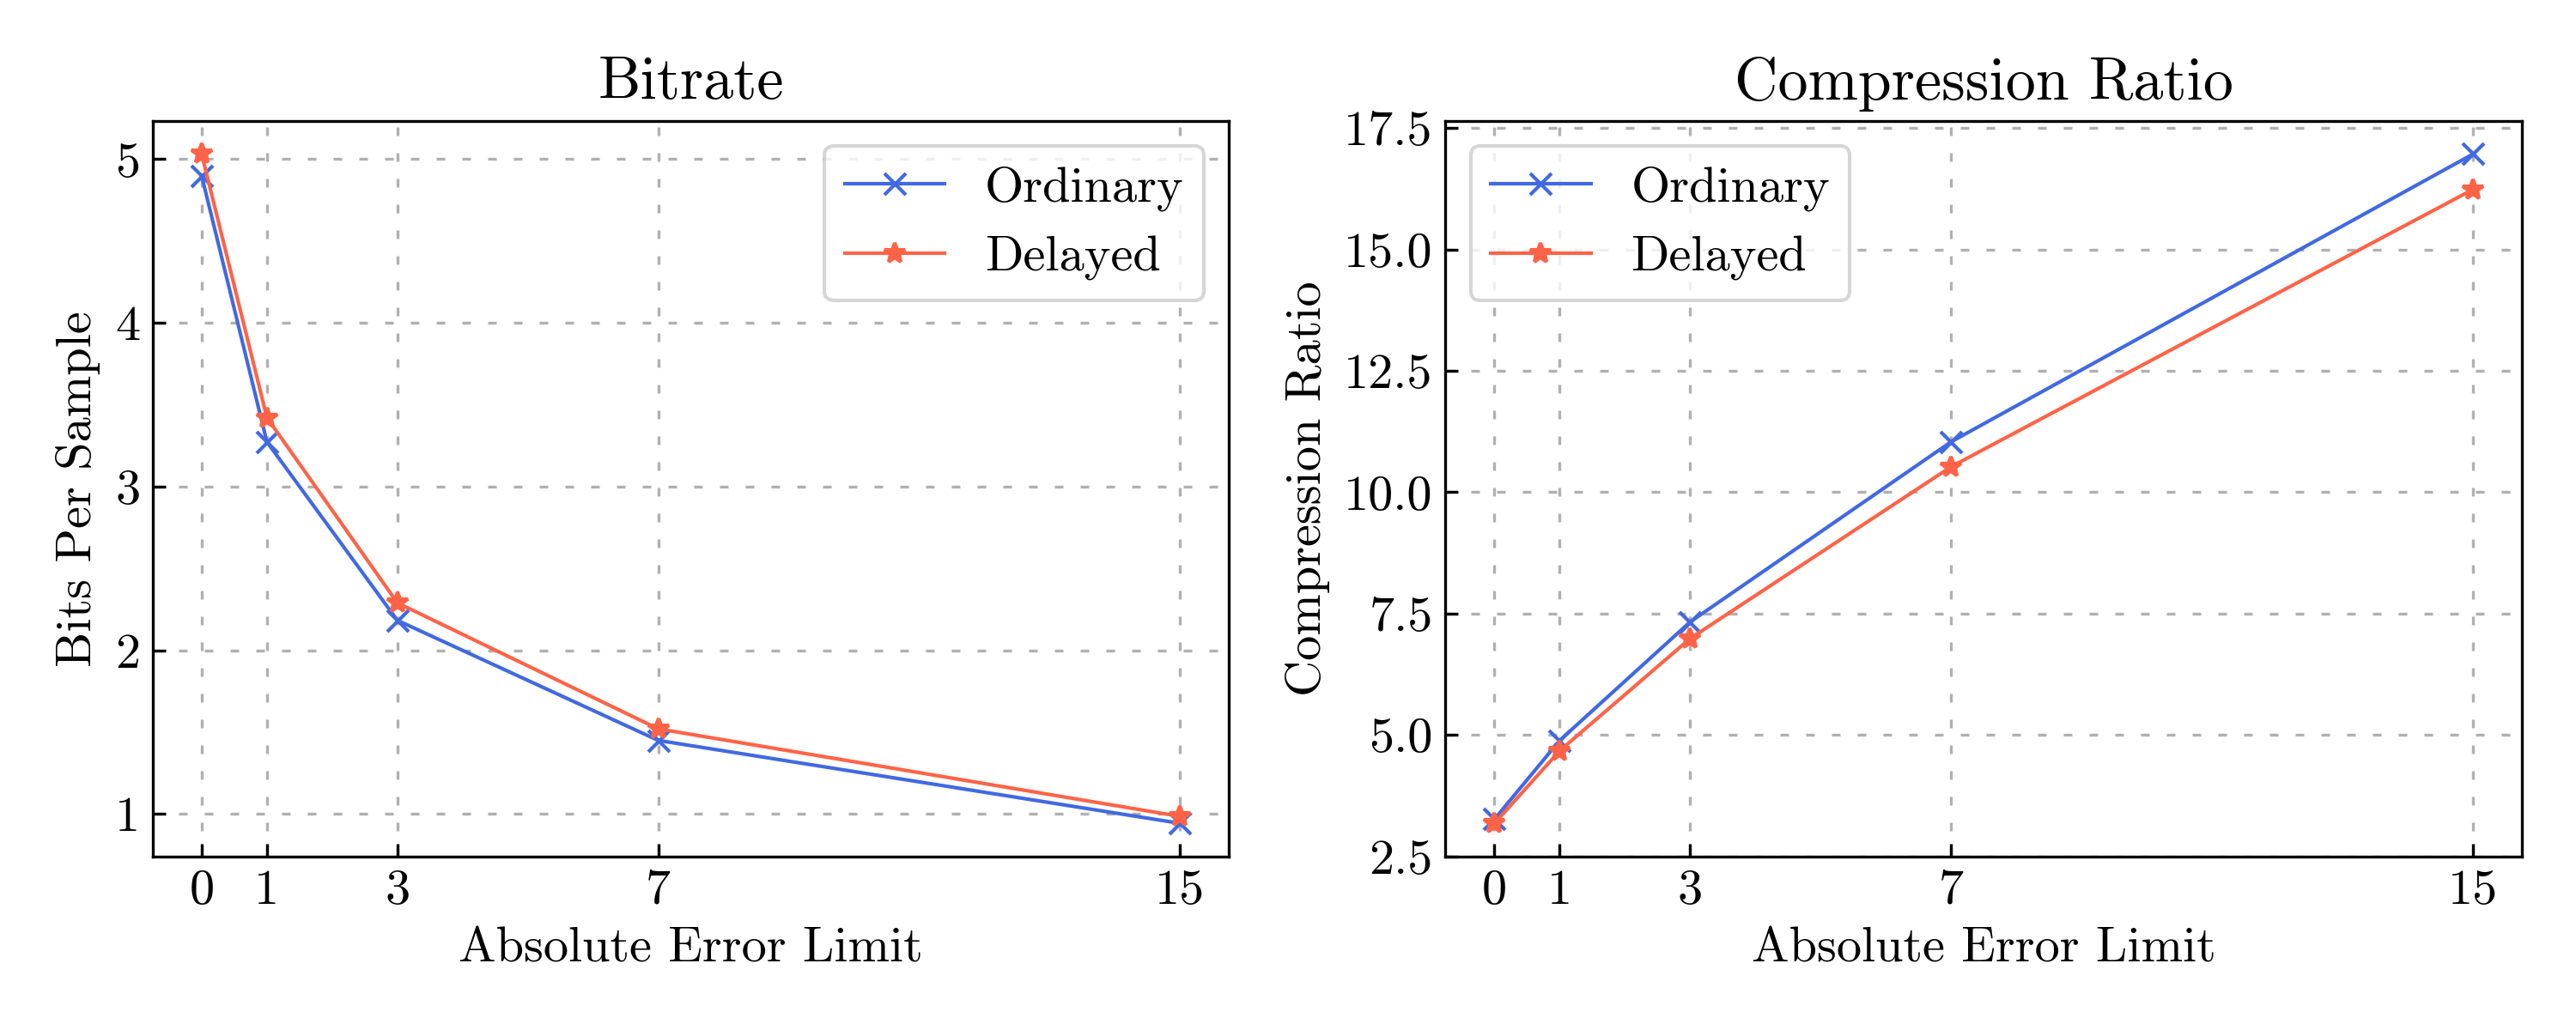
\includegraphics[width=1\textwidth]{figures/compression_performance_aviris.png}
	\end{center}
	\caption{Compression performance presented in bits per sample and compression ratio for a set of absolute error limits. Results are averaged over AVIRIS Yellowstone image set with $D=16$.}
	\label{fig:compression-performance-aviris}
\end{figure}

\begin{table}[ht]
	\caption{PSNR of decompressed images averaged over ten coastline images from HYPSO-2 for a set of PAEs.}
	\label{tab:psnr-compared}
	\begin{center}
		\begin{tabular}{lrr}
			\hline
			\textbf{PAE} & \textbf{CR} & \textbf{PSNR (dB)} \\
			\hline
			0            & 1.995       & N/A                \\ % 2.03            -> 2.02
			1            & 2.488       & 225.86             \\ % 2.55 (225.86dB) -> 2.53 (225.86dB)
			3            & 3.077       & 207.95             \\ % 3.17 (207.95dB) -> 3.15 (207.94dB)
			7            & 3.912       & 192.55             \\ % 4.07 (192.54dB) -> 4.03 (192.54dB)
			15           & 5.219       & 178.08             \\ % 5.45 (178.10dB) -> 5.39 (178.10dB)
			\hline
		\end{tabular}
	\end{center}
\end{table}

\autoref{tab:psnr-compared} shows the \acrshort{PSNR} of reconstructed \acrshort{hypso}-2 images compressed using delayed weight updates. For the lossless mode, reconstructed images are identical. As \acrshort{PAE} increases, the \acrshort{PSNR} drops. Quality of the reconstructed images is not affected by the weight update scheme, and thus the \acrshort{PSNR} for images compressed with the standard compliant weight updates are identical to those of the table.

As opposed to \citeauthor{jiaRemovalFeedbackLoop2025}, this work keeps weights constant across the first samples of each line, rather than each band (\autoref{eq:delayed-weight-updates-modified}). The penalty on compression performance of this modification is evaluated using the verification model. Results are summarized in \autoref{tab:band-line}, and show an insignificant reduction in performance for \acrshort{hypso}-2 coastline images.

\begin{table}[ht]
	\caption{Keeping weights at the start of every line compared with keeping weights only at the start of every band.}
	\label{tab:band-line}
	\begin{center}
		\begin{tabular}{lrr}
			\hline
			\textbf{PAE} & \textbf{Line} & \textbf{Band} \\
			\hline
			0            & 1.995         & 1.995         \\
			1            & 2.488         & 2.488         \\
			3            & 3.077         & 3.078         \\
			7            & 3.912         & 3.913         \\
			15           & 5.219         & 5.219         \\
			\hline
		\end{tabular}
	\end{center}
\end{table}

\begin{figure}[ht!]
	\begin{center}
		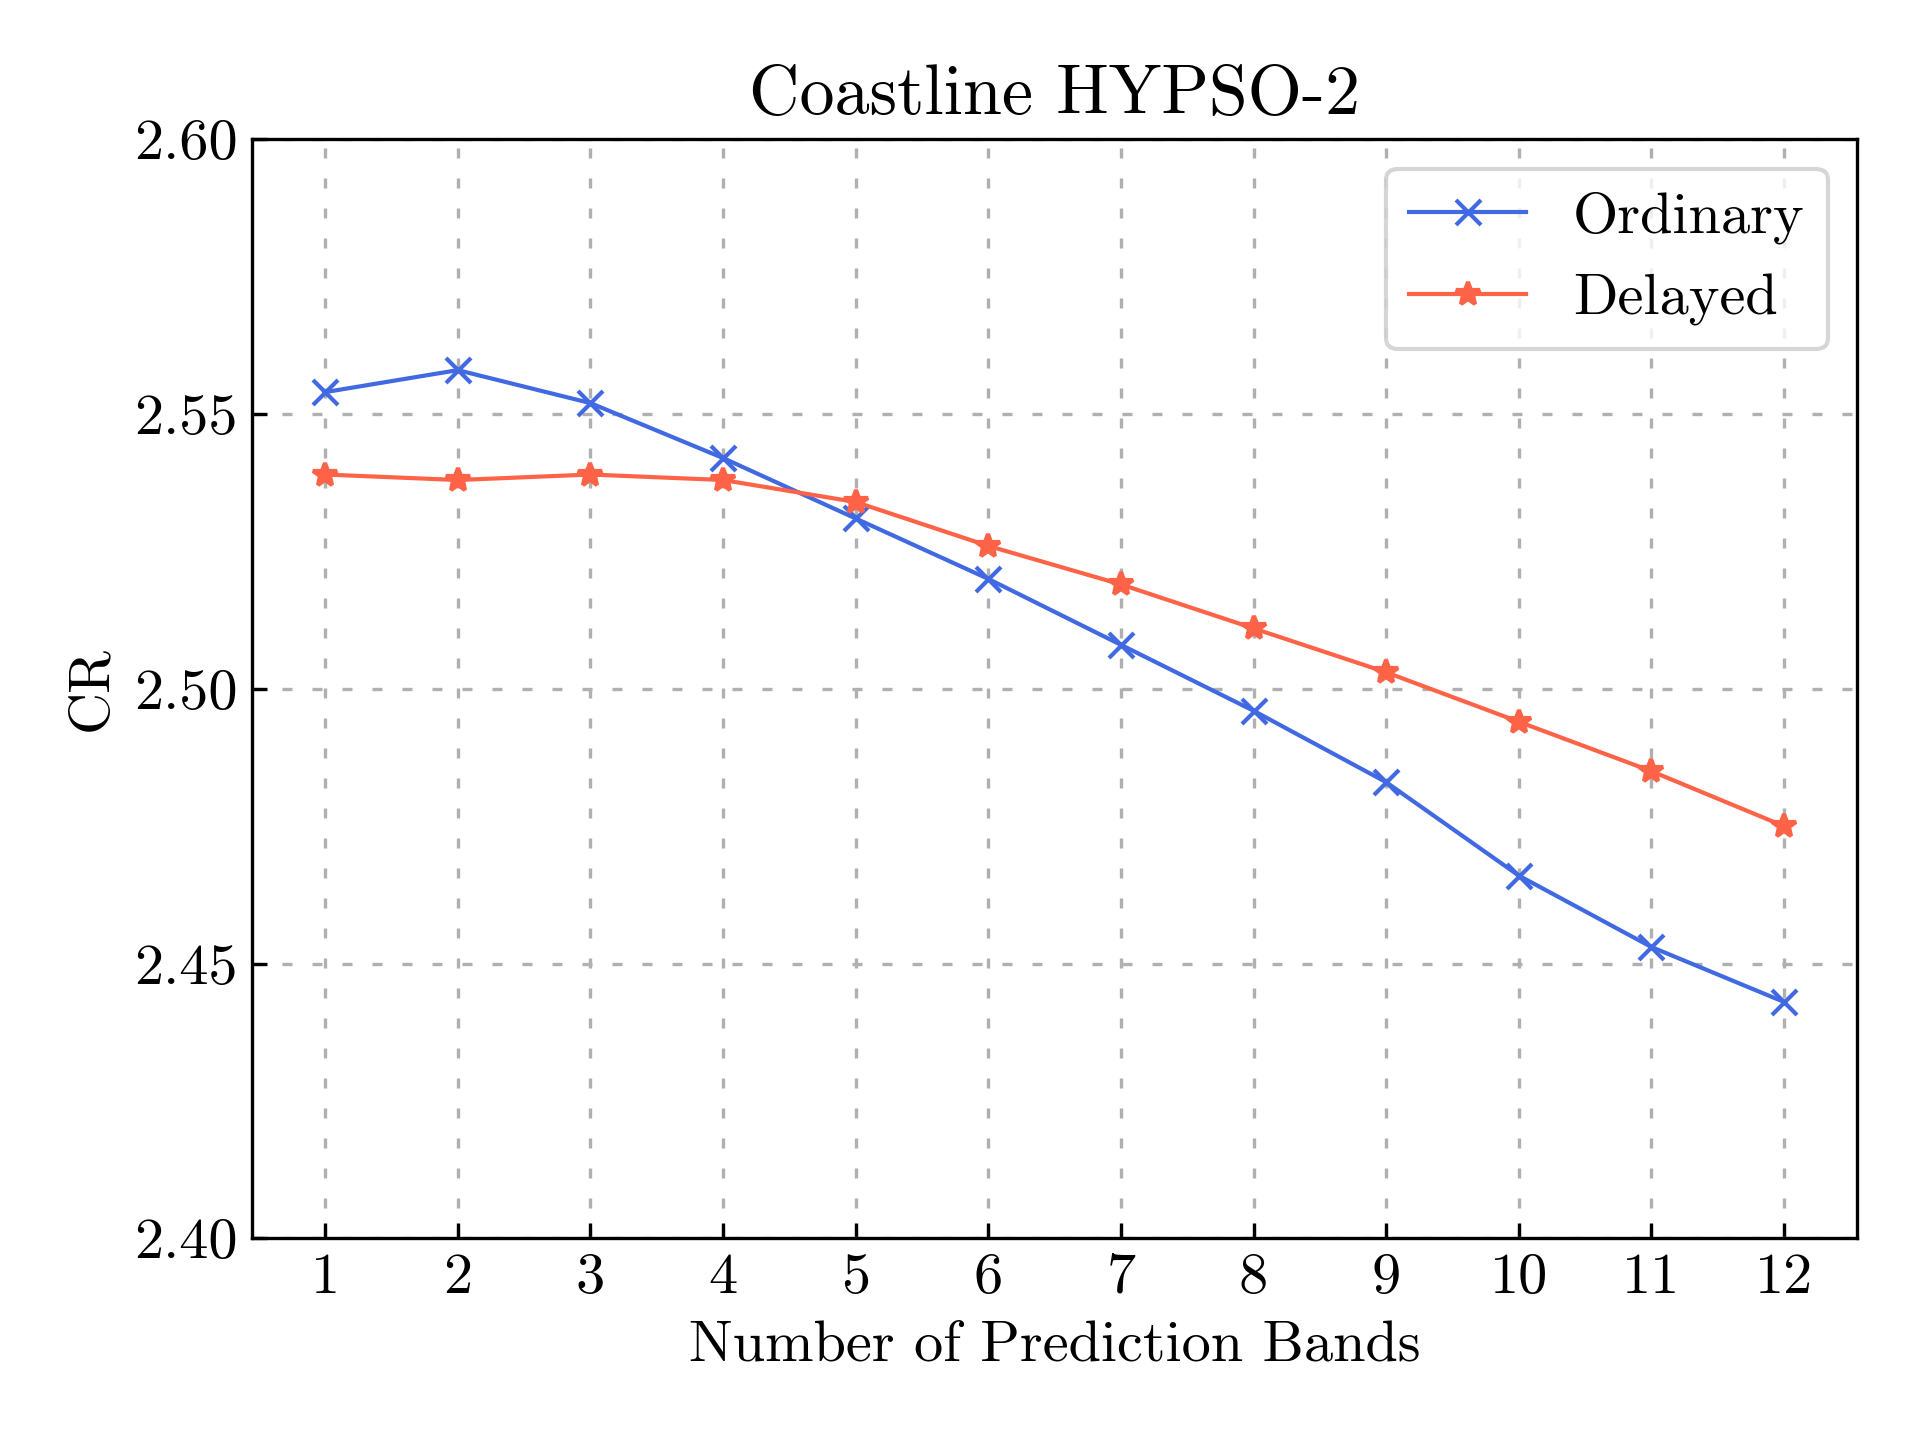
\includegraphics[width=0.6\textwidth]{figures/prediction_bands.png}
	\end{center}
	\caption{Compression performance with $r_z=16$ and $a_z=4$ for different numbers of prediction bands $P$, with and without delayed weight updates. Results are averaged over a set of ten HYPSO-2 coastline images.}
	\label{fig:prediction_bands}
\end{figure}

\autoref{fig:prediction_bands} shows compression ratios with and without delayed weight updates for a range of different numbers of prediction bands. Tests are run for the \acrshort{hypso}-2 image set, with $a_z=4$ and $r_z=16$. For ordinary weight updates, $P=2$ gives the highest compression ratio, with performance dropping as $P$ increases. Delayed weight updates result in a flatter curve, indicating a lower sensitivity to the number of prediction bands, with $P=3$ providing the best results. Interestingly, delayed weight updates outperforms the ordinary scheme for higher numbers of prediction bands.

\section{RTL Results}

The modified hardware accelerator is evaluated using the configuration shown in \autoref{tab:parameters} for two different \acrshort{FPGA}s: Zynq-7030 and Zynq ZU7EV. Results are summarized in \autoref{tab:performance-results-hw} for the whole compression core and the predictor module only. The design is evaluated on hardware resource utilization and estimates of the maximum clock frequency based on static timing analysis. For the Zynq-7030 a maximum clock frequency of 92.6 MHz is reached, and 202 MHz for the Zynq ZU7EV, with the latter reaching realtime processing speed. The predictor module only achieves a significantly higher clock frequency, reaching 351 MHz for the Zynq ZU7EV.

Estimates of the power consumption increase with clock frequency, with 284 mW at the lowest, and 1282 mW at the highest. Different \acrshort{FPGA}s also give different power consumptions at the same frequency, something that is not analysed in this work. The compressor maintains a small area footprint, although slightly larger than that of \citeauthor{vorhaugHyperspectralImageCompression2024}, with 6349 \acrshort{LUT}s and 3480 \acrshort{FF}s for the Zynq ZU7EV.

\begin{table}[ht]
	\caption{Resource utilization, power, and maximum clock frequency of the issue 2 hardware accelerator for two different FPGAs, both for the whole accelerator and only the predictor module.}
	\label{tab:performance-results-hw}
	\begin{center}
		\begin{tabular}{lrrrrrr}
			\hline
			\textbf{FPGA}          & \textbf{LUT} & \textbf{FF} & \textbf{DSP} & \textbf{BRAM} & \textbf{Power} & \textbf{Frequency} \\
			\hline
			Zynq-7030              & 5969         & 3463        & 4            & 83.5          & 284 mW         & 92.6 MHz           \\
			Zynq ZU7EV             & 6349         & 3480        & 4            & 79.5          & 890 mW         & 202.0 MHz          \\
			Zynq-7030 (predictor)  & 2866         & 2250        & 4            & 69.5          & 419 mW         & 137.0 MHz          \\
			Zynq ZU7EV (predictor) & 2807         & 2244        & 4            & 69.5          & 1282 mW        & 350.9 MHz          \\
			\hline
		\end{tabular}
	\end{center}
\end{table}

Static timing analysis shows that the critical path of the updated design lies between the predictor and hybrid encoder modules. The starting point is the shift register buffer for the control signal record in the predictor, which follows the processed sample through the pipeline. The critical path terminates in one of the codeword tables for low-entropy codes in the hybrid encoder. Since the critical path is related to the encoder module, higher clock frequency is achieved for the predictor module in isolation. After splitting the sample representative calculation of stage D+9 (\autoref{fig:new-stageD9}), the critical path of the predictor is once again in the weight update calculation. The path starts and ends at the register storing weights $\omega_z^{(i)}(t)$ for weight updates within lines, shown on the right side of \autoref{fig:weights-hw}. Outputs from the register are processed through the refinement step and clipping before looping back to the register input (\autoref{fig:weights-pipeline-hw}).

\section{On-Board Results}

\begin{figure}[b!]
	\begin{center}
		\efbox{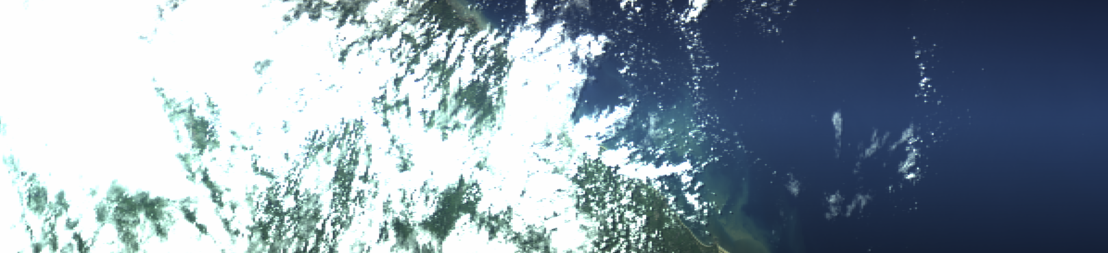
\includegraphics[width=0.8\textwidth]{figures/hypso2-rgb/marceio_onboard_test.png}}
	\end{center}
	\caption{Image captured by the \acrshort{hypso}-2 satellite and compressed on-board using the modified hardware accelerator. The compressed bitstream was decompressed on-ground using the verification model.}
	\label{fig:onboard-test}
\end{figure}

The modified hardware accelerator was tested on-ground using the \acrshort{hypso}-2 engineering model with the configuration presented in \autoref{tab:parameters}. All images from the \acrshort{hypso}-2 coastline set were compressed by hardware, giving identical results as the verification model. After on-ground testing, the design was uplinked to the \acrshort{hypso}-2 satellite. An image of dimensions $N_z=120$, $N_y=598$ and $N_x=1092$ was captured at $8$ frames per second. The image was compressed on-board using the hardware accelerator running at a clock frequency of 92 MHz, downlinked and decompressed on-ground using the verification model. Additionally, the same image was compressed using on-board issue 1 compliant software and downlinked. Using issue 1, the image was compressed with a compression ratio of $2.03$, whereas issue 2 with delayed weight updates achieved a ratio of $2.50$.

The decompressed image, using issue 2, is shown in \autoref{fig:onboard-test}. White areas in the image are clouds which have a high reflection of incoming light, resulting in oversaturated image pixels. The visible coastline in the image is located in Marceió, Brazil. Visual inspection of the decompressed image from issue 1 and 2 show that the accelerator worked on-board the satellite.


% unused tables


% \begin{table}[ht]
% 	\caption{\acrshort{CPU} time and memory use profile for image compression using C++ predictor and reduced memory usage.}
% 	\label{tab:profile-new}
% 	\begin{center}
% 		\begin{tabular}{lrr}
% 			\hline
% 			\textbf{Module} & \textbf{CPU Time} & \textbf{Memory Use} \\
% 			\hline
% 			Total           & 9.4s              & 438MB               \\
% 			Loading         & 0.9\%             & 17.2\%              \\
% 			Predictor       & 72.6\%            & 13.8\%              \\
% 			Hybrid encoder  & 26.4\%            & 69.0\%              \\
% 			Save outputs    & <0.1\%            & N/A                 \\
% 			\hline
% 		\end{tabular}
% 	\end{center}
% \end{table}

% \begin{table}[ht]
% 	\caption{Performance of compression using verification model with C++ predictor and delayed weight updates for single image tests from HYPSO-2, AVIRIS and Landsat with $r_z=16$ and $a_z=4$.}
% 	\label{tab:performance-results-hlm-compress-cpp}
% 	\begin{center}
% 		\begin{tabular}{lrrrrr}
% 			\hline
% 			\textbf{Image} & \textbf{Predictor} & \textbf{Samples} & \textbf{Time (s)} & \textbf{Throughput (MS/s)} & \textbf{Memory (MB)} \\
% 			\hline
% 			HYPSO-2        & C++                & 78361920         & 821               & 0.095                      & 32415                \\ % & (293)
% 			AVIRIS         & C++                & 77643776         & 1166              & 0.066                      & 32091                \\ % & (290)
% 			Landsat        & C++                & 6291456          & 103               & 0.061                      & 2669                 \\ % & (22)
% 			\hline
% 		\end{tabular}
% 	\end{center}
% \end{table}

% \begin{table}[ht]
% 	\caption{Performance of decompression using verification model with C++ predictor and delayed weight updates for single image tests from HYPSO-2, AVIRIS and Landsat with $r_z=16$ and $a_z=4$.}
% 	\label{tab:performance-results-hlm-decompress}
% 	\begin{center}
% 		\begin{tabular}{lrrrr}
% 			\hline
% 			\textbf{Image} & \textbf{Samples} & \textbf{Time (s)} & \textbf{Throughput (MS/s)} & \textbf{Memory (MB)} \\
% 			\hline
% 			Hypso 2        & 78361920         & 1093              & 0.072                      & 32414                \\
% 			AVIRIS         & 77643776         & 1834              & 0.042                      & 32091                \\
% 			Landsat        & 6291456          & 149               & 0.042                      & 2667                 \\
% 			\hline
% 		\end{tabular}
% 	\end{center}
% \end{table}

% \begin{table}[ht]
% 	\caption{Performance of compression using verification model with Python predictor and delayed weight updates for single image tests from HYPSO-2 and Landsat with $r_z=16$ and $a_z=4$.}
% 	\label{tab:performance-results-hlm-compress-py}
% 	\begin{center}
% 		\begin{tabular}{lrrrrr}
% 			\hline
% 			\textbf{Image} & \textbf{Predictor} & \textbf{Samples} & \textbf{Time (s)} & \textbf{Throughput (MS/s)} & \textbf{Memory (MB)} \\
% 			\hline
% 			HYPSO-2        & Python             & 78361920         & 2818              & 0.027                      & 38996                \\ % & (2169)
% 			Landsat        & Python             & 6291456          & 263               & 0.024                      & 3204                 \\ % & (161)
% 			\hline
% 		\end{tabular}
% 	\end{center}
% \end{table}

% \begin{table}[ht]
% 	\caption{Reductions in compression performance for coastline image for this work and the work by \citeauthor{jiaRemovalFeedbackLoop2025}.}
% 	\label{tab:cr-compared}
% 	\begin{center}
% 		\begin{tabular}{lrr}
% 			\hline
% 			PAE & Coastline, \citeauthor{jiaRemovalFeedbackLoop2025} & Coastline, this work \\
% 			\hline
% 			0   & $-1.53\%$                                          & $-0.371\%$           \\ % 2.03            -> 2.02
% 			1   & $-2.88\%$                                          & $-0.470\%$           \\ % 2.55 (225.86dB) -> 2.53 (225.86dB)
% 			3   & $-3.86\%$                                          & $-0.565\%$           \\ % 3.17 (207.95dB) -> 3.15 (207.94dB)
% 			7   & $-4.30\%$                                          & $-0.739\%$           \\ % 4.07 (192.54dB) -> 4.03 (192.54dB)
% 			15  & $-1.23\%$                                          & $-0.826\%$           \\ % 5.45 (178.10dB) -> 5.39 (178.10dB)
% 			\hline
% 		\end{tabular}
% 	\end{center}
% \end{table}

% \begin{figure}[ht]
% 	\begin{center}
% 		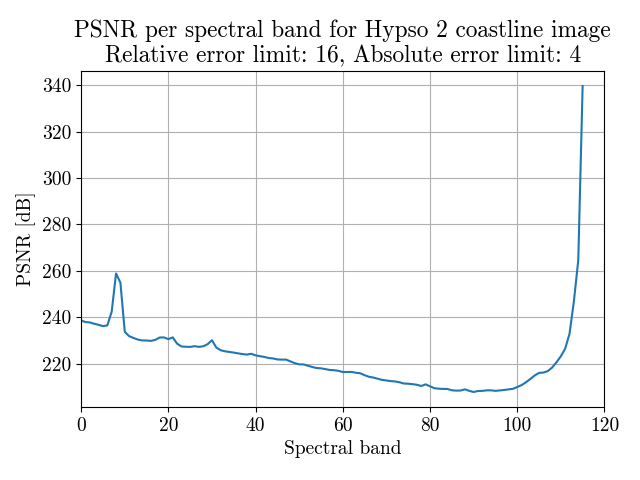
\includegraphics[width=0.65\textwidth]{figures/relative-psnr-coastline.png}
% 	\end{center}
% 	\caption{}
% 	\label{fig:relative-psnr-coastline}
% \end{figure}

% \begin{table}[ht]
% 	\caption{Reduction in compression performance for single image tests with $r_z=16$ and $a_z=4$.}
% 	\label{tab:performance-results-hlm-dw}
% 	\begin{center}
% 		\begin{tabular}{lrrrr}
% 			\hline
% 			\textbf{Image} & \textbf{Ordinary} & \textbf{Delayed} & \textbf{Decrease} \\
% 			\hline
% 			HYPSO-2        & 2.49              & 2.47             & $-0.80\%$         \\
% 			AVIRIS         & 4.41              & 4.31             & $-2.23\%$         \\
% 			Landsat        & 5.21              & 4.82             & $-7.49\%$         \\
% 			\hline
% 		\end{tabular}
% 	\end{center}
% \end{table}

\chapter{Discussion and Further Work}
\label{sec:discussion}

\section{Verification Model Performance}

As shown by tables \ref{tab:coastline-compress} and \ref{tab:coastline-compress-py}, the new C++ predictor greatly outperforms the old Python predictor in terms of execution time. A factor seven improvement is achieved for the predictor, resulting in an improvement factor between $2$ and $4$ depending on the absolute error limit. As the error limit increases, the execution time of the encoder module increases, taking up a greater percentage of the total execution time. This diminishes the improvement due to the new predictor.

The increase in execution time of the encoder for higher absolute error limits is likely due to the increased number of samples that are encoded using low-entropy codes. This is caused by lower entropy of prediction residuals for higher error limits. The codewords of high-entropy codes can be calculated on-the-fly, resulting in fast execution time. However, the \acrshort{V2V} codes used for low-entropy samples require codeword tables, adding additional lookup time. By use of specialized algorithms for binary tree lookups, additional improvements to execution time might be gained.

The verification model by \citeauthor{vorhaugHyperspectralImageCompression2024} stores all intermediate values for both the predictor and encoder modules. By use of the sampler class (\autoref{sec:implementation}), the new predictor allows selectively storing intermediates, reducing the memory requirements. Additionally, storing of most intermediate values of the encoder module has been made optional. Detailed analysis of the memory usage of the verification model has not been performed in this work. However, before modification, the compressor was not able to operate on full \acrshort{hypso}-2 images, $N_z=120$, $N_y=598$ and $N_x=1092$, on a machine with 64 GB of memory. With reduced memory requirements, peak allocated memory for \acrshort{hypso}-2 images range between 30 and 40 GB. This is still a large amount of memory, but is low enough that successful evaluation of the delayed weight update scheme could be performed.

For use in the \acrshort{hypso} mission, compression is performed using the on-board hardware accelerator. This means that the verification model is not needed for compression during the acquisition of images. However, for on-ground decompression when the delayed weight update scheme is used, compliant software is required. This prompts the need for improving the execution time of the verification model, as the execution times (\autoref{tab:coastline-decompress}) upwards of half an hour ($~2000$ seconds) are unacceptable. As shown by the rewritten predictor module, rewriting the hybrid encoder module to C++ can provide great performance improvements, and is therefor suggested. Additionally, specialized algorithms for lookup in \acrshort{V2V} codeword tables should be utilized.

The encoder module uses large arrays that are modified and accessed in-place during calculations. A similar scheme was used by the Python predictor, but is somewhat mitigated by the sampler class of the C++ predictor. However, values needed by complex data dependencies, such as sample representatives and weight updates, are still stored in large arrays. Moving large amounts of data in and out of the memory caches for access is slow, placing a large execution time penalty on the program. In order to remove most of the required memory, and improve execution time, the use of specialized buffers should be employed. These buffers would be similar to those used by the hardware accelerator of \citeauthor{vorhaugHyperspectralImageCompression2024}, storing and providing only values that are needed for calculations. Additional memory can be saved by use of C++ type templates that select the required data type based the dynamic range of the image that is processed.

\section{Compression Performance}

As shown by \autoref{tab:coastline-reduction}, the reduction in compression performance due to delayed weight updates is minimal for the \acrshort{hypso}-2 coastline image set, at less than one percent. The performance penalty for the AVIRIS Yellowstone set is significantly larger, at over four percent for the selected error limits. This is likely due to higher correlation between image samples, such that the images are well suited for predictive compression. The higher compression ratios that are achieved for these images, as shown in figures \ref{fig:compression-performance-hypso} and \ref{fig:compression-performance-aviris}, support this.

The quality of the weight update scheme does not affect the quality of the reconstructed images. This is because the quantizer and prediction loop guarantee that image samples can be reconstructed with at most $m_z(t)$ of error (\autoref{sec:compression}). Weight updates affect the accuracy of the predicted sample values, and thus the entropy of the prediction residuals. This, in turn, affects the achievable compression performance. For images with high correlation between samples, such as the AVIRIS Yellowstone set, the quality of the weight vectors is of higher importance. This results in the greater performance penalty due to the delayed weight updates that is observed as compared to the \acrshort{hypso}-2 images.

Comparing the compression performance of this work with the results of \citeauthor{jiaRemovalFeedbackLoop2025} is challenging. The work does not mention in detail the configurations that are used for compression, other than reduced prediction mode and narrow local sums. Additionally, AVIRIS images are grouped into categories depending on image characteristics such as coastline and urban. However, the exact image groups are not mentioned. By averaging the results of \citeauthor{jiaRemovalFeedbackLoop2025} for AVIRIS images, a reduction of compression performance between one and four percent is given. These number lie in a similar range as those achieved for AVIRIS Yellowstone images of this work (\autoref{tab:coastline-reduction}).

Compression performance is greatly dependant on the selected configurations for the issue 2 algorithm. Furthermore, results depend on the applicable image sensor and characteristics of the image motive. The configuration used for the evaluations of this work is based on the extensive analysis by \citeauthor{blanesPerformanceImpactParameter2019} \cite{blanesPerformanceImpactParameter2019}. Additionally, a simple analysis is made here to find the most suited number of prediction bands for \acrshort{hypso}-2 images. This is due to the direct impact of this parameter on the area footprint of the hardware accelerator, as shown by \citeauthor{vorhaugHyperspectralImageCompression2024} \cite{vorhaugHyperspectralImageCompression2024}. Results using both ordinary and delayed weight updates correspond well to the value suggested by \citeauthor{blanesPerformanceImpactParameter2019}, as shown in \autoref{fig:prediction_bands}, with the optimal value being $P=2$ or $P=3$.

\autoref{tab:psnr-compared} shows how the \acrshort{PSNR} of reconstructed \acrshort{hypso}-2 images drops as the absolute error limit is increased, starting as 226 dB for $a_z=1$. As mentioned, the quality of the reconstructed images is not affected by the weight update scheme. Selecting the correct error limits is a tradeoff between the desired compression ratio and the required quality of reconstructed images. Some work has been done to analyse the effects of lossy compression on hyperspectral images, such as \cite{chen2019compression, garcia2020competitive, garciavilchez2010impact}, but the threshold for acceptable loss varies on the usecases of the images. Finding suitable error limits for use in the \acrshort{hypso} mission requires extensive analysis, and is outside the scope of this work.

\section{Verification Coverage}

Coverage data from randomly generated tests was collected and is presented in \autoref{app:verification-coverage}.

A large number of possible corner cases exists, so it is impossible to do extensive testing.

\section{RTL Results}

Why is it so small?

Band dependant error limits?

Further improvements: hybrid encoder, there exists better performing implementations.

Moving around the calculations of the weight update pipeline to further increase throughput.

Packer and reorder buffers do not need work as they have higher top speeds as found by Vorhaug.

\section{Place in State-of-the-art}

\begin{table}[ht]
	\caption{Hardware utilization and throughput of hardware accelerators of the issue 2 standard. The predictor module is the smallest and fastest in open literature.}
	\label{tab:throughput-this-work}
	\centering
	\begin{tabular}{l r r r r r r}
		\hline
		\textbf{Implementation}                                                                                      & \textbf{FPGA} & \textbf{LUT} & \textbf{FF} & \textbf{DSP} & \textbf{BRAM} & \textbf{Throughput} \\
		\hline
		Barrios et al.\ \cite{barriosHardwareImplementationCCSDS2021}                                                & XCKU040       & 17185        & 11915       & 63           & 85            & 18~MS/s             \\
		B\'ascones et al.\ \cite{basconesRealTimeFPGAImplementation2022}                                             & XQRKU060      & 16458        & 15707       & 30           & 187.5         & 285~MS/s            \\
		Chatziantoniou et al.\ \cite{chatziantoniouScalableDataRateNearLossless2022a} 1 core                         & XCKU040       & 18861        & 21395       & -            & 104           & 285~MS/s            \\
		Chatziantoniou et al.\ \cite{chatziantoniouScalableDataRateNearLossless2022a} 5 core                         & XCKU040       & 67362        & 68987       & -            & 306           & 1375~MS/s           \\
		S\'anchez et al.\ \cite{sanchezReducingDataDependencies2022, barriosRemovingDataDependencies2024}, predictor & XCKU040       & 19840        & 12970       & 33           & 213           & 231~MS/s            \\
		Barrios et al.\ \cite{barriosRemovingDataDependencies2024}, predictor                                        & XCKU040       & 11095        & 11729       & 20           & 186.5         & 236~MS/s            \\
		Vorhaug et al.\ \cite{vorhaugHyperspectralImageCompression2024}                                              & XCKU040       & 5577         & 2635        & 4            & 57.5          & 110~MS/s            \\
		Vorhaug et al.\ \cite{vorhaugHyperspectralImageCompression2024}                                              & XCZU7EV       & 5475         & 2635        & 4            & 57.5          & 141~MS/s            \\
		Jia et al.\ \cite{jiaRemovalFeedbackLoop2025}, predictor                                                     & XCZU5EV       & 3995         & 5050        & 7            & 94            & 348~MS/s            \\
		This work                                                                                                    & XCZU7EV       & 6349         & 3480        & 4            & 79.5          & 202~MS/s            \\
		This work, predictor                                                                                         & XCZU7EV       & 2807         & 2244        & 4            & 69.5          & 351~MS/s            \\
		\hline
	\end{tabular}
\end{table}

\section{CCSDS 123.0-B-2 Compliance}

With delayed weight updates we are not compliant...

Minimum x-size is now D+13 due to pipeline depth and size of sample representative and local difference buffers.

\section{On-board Testing}

The successful on-board compression, downlink and decompression of an image from the \acrshort{hypso}-2 satellite shows that the delayed weight update scheme is a viable solution for increased throughput of issue 2 accelerators. The updated design was run at a clock frequency of 92 MHz on the Zynq-7030, matching the frequency estimate given by static timing analysis. The original design by \citeauthor{vorhaugHyperspectralImageCompression2024} was tested on-board \acrshort{hypso}-1, and ran at a lower frequency of 50 MHz. Future improvements to the design should aim at reaching 100 MHz, which would allow the removal of the additional clocking wizard block as the surround systems run at this frequency.

During integration for \acrshort{hypso}-2 an error was encountered in which the accelerator produced the wrong outputs. This turned out to be caused by the wrong selection of byte endianness on the output transmitted by the \acrshort{AXI} bus. The final image files that are stored to the on-board SD-card use the big endian byte order. Because of this it was assumed that the same ordering should be used for transmission on the output data bus. This assumption proved wrong, and little endian had to be used. At some point in the on-board image processing between retrieval from the compressor and storage, the byte order is switched.

Bug in hardware that was not detected by simulation. Internal register that needs to be reset between each compression, likely due to requiring some initial value for the calculations. Solved by reprogramming fpga between runs.

The decrease in compression performance introduced by delayed weight updates cause significantly longer downlink time which is not outweighed by the reduced execution time, by far.

Work should be done to properly integrate the issue 2 implementation into the HYPSO-2 on-board-processing (OPU) system. This includes writing software for header, and selection of parameters. As of now, HYPSO-2 still uses the outdated issue 1 implementation. Although fast, it cannot achieve compression rates close to those of issue 2. Issue 2 for HYPSO-3!! Header software should be written in C, for easy integration with the existing software.

\chapter{Conclusions}
\label{sec:conclusion}

Small satellite technology has increased the availability of remote sensing data such as hyperspectral imagery. The image sensor on-board the \acrshort{hypso} missions developed at \acrshort{NTNU} capture images of 120 spectral bands, producing large amounts of data that must be downlinked with limited bandwidth. On-board image compression is needed to effectively handle image data, and is typically implemented as hardware accelerators running on flexible \acrshort{FPGA}s.

The CCSDS 123.0-B-2 compression algorithm (issue 2) supports near-lossless compression capable of high compression performance. The complexity of the algorithm, and intersample data dependencies, presents challenges for hardware accelerators that want to optimize hardware resource utilization, throughput and power. Three main approaches have been attempted in the literature to achieve high throughput implementations. \citeauthor{basconesRealTimeFPGAImplementation2022} suggest using a novel sample processing order to interleave data dependant calculations by up to $N_z$ samples. Using VHDL \acrshort{RTL} the approach reaches a throughput of 285 MS/s, but at a large area footprint of 16458 \acrshort{LUT}s and 15707 \acrshort{FF}s. \citeauthor{chatziantoniouScalableDataRateNearLossless2022a} and \citeauthor{valsesiaHighThroughputOnboardHyperspectral2019} suggest using prequantization, in place of the in-loop quantizer of the standard. This approach matches the throughput of \citeauthor{basconesRealTimeFPGAImplementation2022}, but at a penalty in compression performance and even greater area footprint. \citeauthor{sanchezReducingDataDependencies2022} suggest a mathematically equivalent method for calculating the sign of the double-resolution prediction error needed for updating the adaptive weight vector of the prediction loop. This, combined with using reduced prediction mode, narrow local sums and the \acrshort{BIL} processing order, allows implementation of a pipeline that is limited by the weight update calculation. Using this approach, \citeauthor{vorhaugHyperspectralImageCompression2024} designs a compression core reaching a throughput of 110 MS/s with the smallest area footprint at 5577 \acrshort{LUT}s and 2635 \acrshort{FF}s. The design is successfully tested on-board the \acrshort{hypso}-1 satellite. To alleviate the critical path of the mathematical optimization approach, \citeauthor{jiaRemovalFeedbackLoop2025} suggest a novel weight update scheme, dubbed delayed weight updates, reaching a throughput of 348 MS/s for the predictor module.

This work integrates the delayed weight update scheme into the accelerator designed by \citeauthor{vorhaugHyperspectralImageCompression2024}. The new pipeline reaches 202 MS/s for the Zynq ZU7EV \acrshort{FPGA} with a minimal increase in area for a total of 6349 \acrshort{LUT}s and 3480 \acrshort{FF}s. In isolation, the predictor module reaches 351 MS/s, making it the fastest and smallest implementation in the open literature. The design is successfully tested on-board the \acrshort{hypso}-2 satellite, with a throughput of 92 MS/s on the Zynq-7030. Future improvements to the design should focus on increasing the throughput of the limiting hybrid encoder module.

The new weight update scheme deviates from the issue 2 standard, requiring custom software for decompression. This works presents an open-source, issue 2 compliant decompressor based on the verification model by \citeauthor{vorhaugHyperspectralImageCompression2024} with optional support for delayed weight updates. The new predictor module written in C++ achieves a factor seven improvement in execution time. Further improvements in execution time can be gained in the encoder module and by optimizing memory accesses. The verification module is used to verify the hardware accelerator and decompress its outputs. For \acrshort{hypso}-2 images, the penalty in compression performance due to delayed weight updates is less than one percent, an acceptable tradeoff for the increase in throughput.



\chapter*{\bibname}
\printbibliography[heading=none]

% \appendix
% \chapter{Additional Material}
\label{app:additional}

An appendix

% \cleardoublepage
% 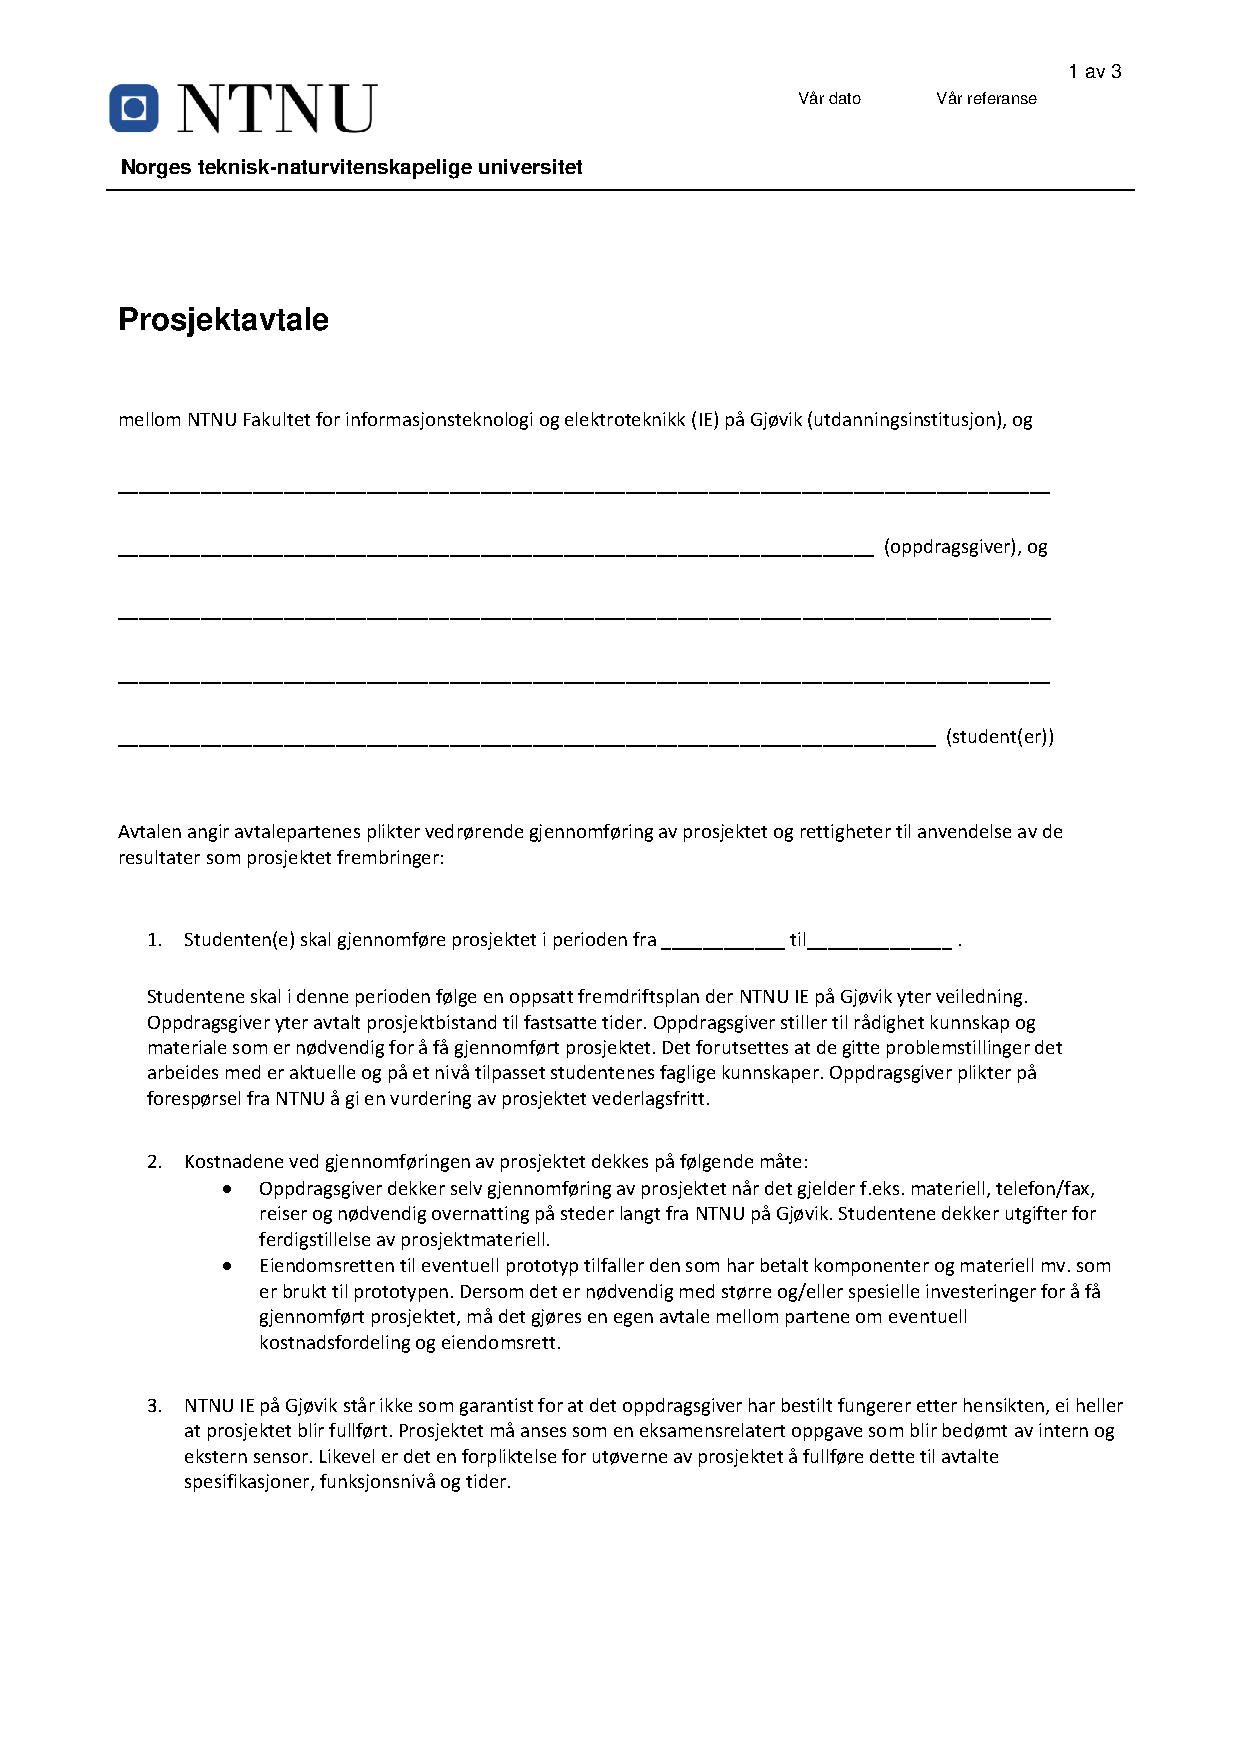
\includepdf[pages=-]{appendices/NTNUProsjektavtale.pdf}


\end{document}
